% Festlegung des allgemeinen Dokumentenformats
\documentclass[a4paper,12pt]{article}

% Schrift
\usepackage[T1]{fontenc}
\usepackage{lmodern}
\usepackage[utf8]{inputenc}
\usepackage[ngerman]{babel}

% Bilder
\usepackage{graphicx}
% \usepackage[draft]{graphicx} % draft for speedup
\usepackage{float}
\graphicspath{{./assets/img}}

% Variablen
% Variablen
\newcommand{\titleDocument}{Masterarbeit}
\newcommand{\subjectDocument}{StudyMap: Konzeption und Evaluierung eines
innovativen Studiengangfinders am Beispiel der OTH-Regensburg}
\newcommand*{\bildquelle}{
  \footnotesize Quelle:
}
\newcommand{\code}[1]{\noindent\ignorespaces\texttt{#1}}

% Code
\usepackage{listings}
\usepackage{color}

\definecolor{black}{rgb}{0,0,0}
\definecolor{dkgreen}{rgb}{0,0.6,0}
\definecolor{gray}{rgb}{0.5,0.5,0.5}
\definecolor{mauve}{rgb}{0.58,0,0.82}

\lstset{literate=%
    {Ö}{{\"O}}1
    {Ä}{{\"A}}1
    {Ü}{{\"U}}1
    {ß}{{\ss}}1
    {ü}{{\"u}}1
    {ä}{{\"a}}1
    {ö}{{\"o}}1
    {~}{{\textasciitilde}}1
}

\lstdefinestyle{Bash} {
  frame=single,
  language=Bash,
  aboveskip=3mm,
  belowskip=3mm,
  showstringspaces=false,
  columns=flexible,
  basicstyle={\small\ttfamily},
  numbers=none,
  numberstyle=\tiny\color{black},
  keywordstyle=\color{black},
  commentstyle=\color{black},
  stringstyle=\color{black},
  breaklines=true,
  breakatwhitespace=true,
  tabsize=3
}

\lstset{emph={\$},emphstyle=\textbf}

\lstdefinestyle{Python} {
  frame=single,
  language=Bash,
  aboveskip=3mm,
  belowskip=3mm,
  showstringspaces=false,
  columns=flexible,
  basicstyle={\small\ttfamily},
  numbers=left,
  numberstyle=\tiny\color{mauve},
  keywordstyle=\color{mauve},
  commentstyle=\color{dkgreen},
  stringstyle=\color{dkgreen},
  breaklines=true,
  breakatwhitespace=true,
  tabsize=2
}

% mehrseitige Tabellen ermöglichen
\usepackage{longtable}
\usepackage{diagbox}

% Packet für Seitenrandabstände und Einstellung für Seitenränder
\usepackage{geometry}
% Internet
%\geometry{left=3.5cm, right=2.5cm, top=2.5cm, bottom=2cm}
% Kern
\geometry{a4paper, top=27mm, left=20mm, right=20mm, bottom=35mm, headsep=10mm,
footskip=12mm}

% bricht lange URLs "schön" um
\usepackage[hyphens,obeyspaces,spaces]{url}

% Festlegung Art der Zitierung
\usepackage{csquotes}
\usepackage[style=apa, backend=biber]{biblatex}
\addbibresource{assets/thesis-2.bib}

% Abstand zwischen Absätze
\setlength{\parindent}{2em}
\setlength{\parskip}{1em}

% Paket für Zeilenabstand
\usepackage{setspace}
\onehalfspacing
% Kern:
% \setstretch{1.15}

% für Bildbezeichner
\usepackage{capt-of}

% für Stichwortverzeichnis
\usepackage{makeidx}

% für Abkürzungsverzeichnis
\usepackage{acronym}

% Für Phantomsection
\usepackage{hyperref}

% Für Tabellen
\usepackage{tabularx}

% Konfiguriere das Inhaltsverzeichnis
\usepackage{tocbasic}

% Anhang: PDF einfügen
\usepackage{pdfpages}

% subsubsubsection durch paragraph
\usepackage{titlesec}
\setcounter{secnumdepth}{4}
\titleformat{\paragraph}
{\normalfont\normalsize\bfseries}{\theparagraph}{1em}{}
\titlespacing*{\paragraph}
{0pt}{3.25ex plus 1ex minus .2ex}{1.5ex plus .2ex}
% Kern:
\titlespacing{\section}{0pt}{12pt plus 4pt minus 2pt}{8pt plus 2pt minus 2pt}
\titlespacing{\subsection}{0pt}{12pt plus 4pt minus 2pt}{6pt plus 2pt minus 2pt}
\titlespacing{\subsubsection}{0pt}{12pt plus 4pt minus 2pt}{4pt plus 2pt minus 2pt}

% \autoref: Subsubsection umbenennen
\addto\extrasngerman{
    \def\subsubsectionautorefname{Unterabschnitt}
}

% Titel
\title{Bachelorarbeit}

% Autor
\author{Andreas Huber}

% Datum
\date{\today}

%
% Start
% des
% Dokuments
%
\begin{document}

% Titelseite
\thispagestyle{empty}

\begin{figure}[t]
 \centering
 
\includegraphics[width=0.4\textwidth]{assets/oth/logo}
\end{figure}

\begin{verbatim}
\end{verbatim}

\begin{center}
    \Large{Ostbayerische Technische Hochschule Regensburg} \\
    \Large{Fakultät für Informatik und Mathematik}
\end{center}

\begin{verbatim}
\end{verbatim}

\begin{center}
    \doublespacing
    \textbf{\huge{\titleDocument}}\\

    \onehalfspacing

    \begin{center}
        Zur Erlangung des akademischen Grades \\ Master of Science (M. Sc.)
    \end{center}

    \begin{verbatim}
    \end{verbatim}

    \begin{doublespace}
        \textbf{\Large{{~\subjectDocument}}}
    \end{doublespace}
\end{center}

\begin{verbatim}
\end{verbatim}

\begin{verbatim}
\end{verbatim}

\begin{flushleft}
    \begin{tabularx}{\linewidth}{@{}>{\bfseries}l@{\hspace{.9em}}X@{}}
        \textbf{Vorgelegt von:} & Andreas Huber <andreas.huber@st.oth-regensburg.de> \\
        \textbf{Matrikelnummer:}& 3370380 \\
        \textbf{Studiengang:}   & Master Informatik (Schwerp. Software Engineering) \\
                                & \\
        \textbf{Erstgutachter:} & Prof. Dr. Markus Heckner \\
        \textbf{Zweitgutachter:}& Prof. Dr. Daniel Jobst \\
                                & \\
        \textbf{Abgabefrist:}   & 20. März 2024 \\
    \end{tabularx}
\end{flushleft}
\newpage

% Einverständniserklärung
\thispagestyle{empty}
\section*{Erklärung zur Masterarbeit}

\bigskip
\bigskip 
\bigskip 

\begin{enumerate}
    \item Mir ist bekannt, dass dieses Exemplar der Abschlussarbeit als Prüfungsleistung in das Eigentum der Ostbayerischen Technischen Hochschule Regensburg übergeht.
    \item Ich erkläre hiermit, dass ich diese Abschlussarbeit selbständig verfasst, noch nicht anderweitig für Prüfungszwecke vorgelegt, keine anderen als die angegebenen Quellen und Hilfsmittel benutzt sowie wörtliche und sinngemäße Zitate als solche gekennzeichnet habe.
\end{enumerate}

\bigskip 
\bigskip 
\bigskip 

\noindent Regensburg, den \today

\bigskip 
\bigskip

\noindent\line(1,0){200}
\newline
\noindent Andreas Huber
\newpage

% Römische Nummerierung
\pagenumbering{Roman}

% Inhaltsverzeichnis
\tableofcontents

% Abbildungsverzeichnis
\newpage
\phantomsection
\addcontentsline{toc}{section}{Abbildungsverzeichnis}
\renewcommand\refname{Abbildungsverzeichnis}

\listoffigures

% Tabellenverzeichnis
\newpage
\phantomsection
\addcontentsline{toc}{section}{Tabellenverzeichnis}
\renewcommand\refname{Tabellenverzeichnis}

\listoftables

% Abkürzungsverzeichnis
\newpage
\phantomsection
\section*{Abkürzungsverzeichnis}
\addcontentsline{toc}{section}{Abkürzungsverzeichnis}

\begin{acronym}[Bash]
    % \acro{bash}[Bash]{Bourne-again shell}
    % \acro{ide}[IDE]{Integrated Development Environment}
    % \acro{ldap}[LDAP]{Lightweight Directory Access Protocol}
    % \acro{lms}[LMS]{Learning Management System}
    % \acro{oth}[OTH]{Ostbayerische Technische Hochschule}
    % \acro{sd}[SD]{Standardabweichung}
\end{acronym}

% Arabische Seitennummerierung ab hier
\newpage
\pagenumbering{arabic}

% Einleitung
\section{Einleitung}\label{einleitung}
\subsection{Einleitung und Motivation}\label{einleitung-und-motivation}
Die Wahl des richtigen Studiengangs ist ein wichtiger Schritt im Leben eines jeden angehenden Studierenden. Sie legt den Grundstein für die akademische und berufliche Entwicklung und beeinflusst den individuellen Bildungsweg maßgeblich. Angesichts der Vielfalt an verfügbaren Studiengängen stehen Studieninteressierte vor einer komplexen Entscheidung, die durch eine breite Palette von Inhalten,  Schwerpunkten und Karrierewegen geprägt ist. Diese Vielzahl an Informationen kann zu Unsicherheit und Verwirrung führen, wodurch nicht selten falsche Studienentscheidungen getroffen werden. \parencite{beckmann_verbesserung_2021}

Die vorliegende Masterarbeit greift dieses weit verbreitete Problem auf und stellt einen innovativen Ansatz zur Studienorientierung vor. Das Ziel ist es, eine benutzerfreundliche, automatisch generierte Infografik-basierte Plattform zu entwickeln, die Studieninteressierte dabei unterstützt, fundierte Entscheidungen über ihren zukünftigen Bildungsweg zu treffen. Die Anwendung namens StudyMap kombiniert moderne Datenanalyse, interaktive Benutzeroberflächen und nutzerzentriertes Design, um den Orientierungsprozess zu optimieren.

\subsection{Problemstellung/Zielsetzung}\label{problemstellung-zielsetzung}
Die derzeitige Studienorientierung wird oft durch eine Informationsflut und eine begrenzte Transparenz der verfügbaren Studiengänge behindert. Häufig kennen Studieninteressierte einen Studiengang oder eine ungefähre Richtung, in die sie gehen möchten. Um ähnliche Studiengänge oder alle Studiengänge in der gewünschten Richtung zu finden, fehlt oft der Überblick. \parencite{beckmann_verbesserung_2021} Diese Unsicherheit kann zu falschen Studienentscheidungen führen, die wiederum Studienabbrüche durch Motivationsmangel zur Folge haben \parencite{heublein_ursachen_2010}.

\noindent
Die spezifischen Ziele dieser Arbeit sind:
\begin{enumerate}
\item Entwicklung eines Konzepts für einen Studiengangsfinder auf Basis einer
interaktiven Infografik-basierten Benutzeroberfläche.
\item Implementierung und technische Umsetzung des entwickelten Systems am
Beispiel der Ostbayerischen Technischen Hochschule Regensburg (OTH-Regensburg).
\item Evaluation und Validierung eines Prototypen durch Tests mit potenziellen
Nutzern und Analyse der Ergebnisse.
\item Diskussion der Stärken und Schwächen des entwickelten Systems sowie der
möglichen Auswirkungen auf die Studienberatung.
\item Die Ergebnisse dieser Arbeit sollen dazu beitragen, die
Studienorientierung für Studieninteressierte zu erleichtern und ihnen bessere
Informationen und Orientierungshilfen zur Verfügung zu stellen.
\end{enumerate}

\subsection{Gliederung der Arbeit}
Die Arbeit beginnt nach der Einleitung mit dem theoretischen Hintergrund. Es werden bereits existierende Werkzeuge und Konzepte zur Studienorientierung beschrieben und die Theorie der Anwendung von interaktiven Systemen definiert.

Anschließend folgt das Kapitel \nameref{sec:methodik}, in dem zunächst verschiedene mögliche Algorithmen zur Darstellung aller Studiengänge besprochen werden. Daran anknüpfend werden die Datenquellen für den Studiengangsfinder hinsichtlich ihrer Herkunft bzw. Beschaffung diskutiert.

Das nächste Kapitel beschreibt das Konzept des innovativen Studiengangsfinders. Zunächst wird die Hochschule Regensburg als Fallbeispiel vorgestellt, einschließlich ihrer Herausforderungen und Ziele. Im Anschluss daran wird ein Konzept entwickelt, wie das Aussehen des Studiengangsfinders sein könnte und wie die Interaktivität gewährleistet werden kann. Außerdem wird in diesem Kapitel die Datenpflege und -sicherung behandelt. Dabei wird explizit auf die Datensicherung, die Trennung von Produktiv- und Testumgebung sowie auf eine Administrationsoberfläche eingegangen.

Das fünfte Kapitel behandelt den User-centered Design Prozess. Anhand von zwei Studien wird das Konzept evaluiert und verfeinert. Die erste Studie ist eine Mockup-Studie, in der das Designkonzept des Studiengangsfinders diskutiert wird. Auf der Grundlage dieser Ergebnisse wird ein Prototyp entwickelt, mit dem eine Prototypstudie mit 40 Personen, die sich für ein Studium interessieren, durchgeführt und diskutiert wird.

Nach Abschluss der Studien wird im Kapitel \nameref{sec:implementierung-und-deployment} zuerst die Auswahl der Technologien besprochen und daraufhin die Herausforderungen, die während der Implementierung entstanden sind. Schließlich werden die erläuterten Einzelkomponenten zusammengeführt und die daraus resultierende Softwarearchitektur, unterteilt in Frontend und Backend, erläutert. Der letzte Abschnitt dieses Kapitels befasst sich mit dem Software-Deployment. Es wird gezeigt, wie das Deployment abläuft, wie getestet werden kann und wie die Software letztendlich bereitgestellt wird.

Abschließend werden im letzten Kapitel die Ergebnisse und die wichtigsten Erkenntnisse zusammengefasst. Darüber hinaus wird ein Vergleich zu anderen Tools im Bereich der Studienorientierung gezogen und ein Ausblick gegeben. Im Rahmen dieses Ausblicks werden mögliche Erweiterungen und Anwendungen für die Zukunft diskutiert.
\newpage

% Theoretischer Hintergrund und vorhandene Studiengangsfinder-Konzepte
\section{Theoretischer Hintergrund und vorhandene Studiengangsfinder-Konzepte}
\subsection{Bisheriges Vorgehen bei der Studienorientierung}
% Wahl des Studiengangs PDF Seite 355
% Hochschulinformationstage wurden von MINT-Studierenden insgesamt häufig zur Studienentscheidung und Studienplanung genutzt (72 %).

% 1. Wichtigster Faktor Fach, 2. Ort o. Hochschultyp
% Oft kennen ein Fach, danach suchen sie einen Ort bzw. eine Hochschule
% Wenn sie dann auf die OTH Seite kommen, können sie nach der Kategorie suchen
% und dann ähnliche vielleicht noch besser passende Studiengänge finden
% Wichtigster Fachwahlgrund: Begabungen und pers. Neigungen
% Was Eltern, Verwandte u. Freunde sagen nur 0,1 %
% (Seite 67 von neuem PDF)
% 5 Typen schon Entscheidern, jeder entscheidet nach Pers. Neigung -> umso
% wichtiger ist es ihnen alle ähnlichen Studiengänge zu präsentieren!

Die Studienorientierung ist ein entscheidender Schritt im Bildungsweg eines
jeden Studieninteressierten und die Entscheidung für ein zukünftiges Studienfach
und eine Hochschule wird traditionell von verschiedenen Faktoren beeinflusst.
Eine umfassende Studie von CHE und EINSTIEG aus dem Jahr 2007 gibt Einblicke in
die Präferenzen und Entscheidungsmuster von Studieninteressierten.

Die Studie zeigt, dass für einen Großteil der Befragten (87,2 \%) die Wahl der
Hochschule und des Hochschulortes weniger relevant ist als das gewählte
Studienfach \parencite{einflussfaktoren}. Dies deutet darauf hin, dass das
persönliche Interesse an einem bestimmten Studienfach die Entscheidung stärker
beeinflusst als die geografische Lage oder der Ruf der Hochschule.

Ein weiteres wichtiges Ergebnis der Studie ist, dass 64,6 \% der Befragten ihr
Studienfach nach ihren Neigungen und Begabungen wählen
\parencite{einflussfaktoren}. Dies verdeutlicht, dass persönliche Neigungen und
individuelle Fähigkeiten die Studienentscheidung maßgeblich beeinflussen.

Die Erkenntnis, dass sich Studieninteressierte bei ihrer Studienfachwahl von
unterschiedlichen Motivationsfaktoren leiten lassen, führt zu der Vorstellung,
dass es verschiedene Entscheidungstypen gibt. Intrinsische Altruisten,
heimatgebundene Hedonisten, serviceorientierte Unabhängige und leistungsstarke
Karriereorientierte sind einige der identifizierten Gruppen, die jeweils
unterschiedliche Prioritäten bei der Fach-, Hochschul- und Ortswahl setzen.
Diese unterschiedlichen Entscheidungsmuster unterstreichen die Vielfalt
individueller Studienmotivationen. \parencite{einflussfaktoren}

In der Praxis bedeutet dies, dass Hochschulen wie die OTH-Regensburg darauf
achten müssen, ihre Studiengänge ansprechend und überzeugend zu präsentieren.
Gerade dann, wenn die Hochschule als mögliche Option in Betracht gezogen wird,
spielt die Möglichkeit, das gewünschte Fach entsprechend der individuellen
Interessen darzustellen, eine entscheidende Rolle.

Ein innovativer Studiengangsfinder, der Fächer inhaltlich kategorisiert und
ähnliche Studiengänge präsentiert, könnte hier eine wichtige Rolle spielen. Mit
einer solchen Lösung könnten Studieninteressierte effektiv über Alternativen
informiert werden, insbesondere wenn der ursprünglich angestrebte Studiengang
nicht verfügbar ist. Dies trägt dazu bei, dass die Hochschule potenzielle
Studierende auch dann überzeugen kann, wenn ihre erste Wahl nicht direkt
verfügbar ist, aber dennoch ähnliche, attraktive Alternativen bietet.


\subsection{Konzepte von Studiengangsfindern}
Die Historie der Studiengangsfinder zeigt eine dominierende Tendenz hin zu
umfragebasierten Konzepten. In diesem Zusammenhang werden Studierende durch
Umfragen zu ihren Interessen, Fähigkeiten und Präferenzen befragt, um auf dieser
Grundlage Studiengangsempfehlungen zu generieren.

Umfragebasierte Studiengangsfinder vertrauen auf die subjektiven Bewertungen
der Nutzer und versuchen, durch direkte Befragungen der Studierenden ihre
Präferenzen zu ermitteln. Die daraus resultierenden Empfehlungen basieren auf
den angegebenen Interessen und Vorlieben. Jedoch sind diese Empfehlungen stark
von der Qualität der gestellten Fragen und der Interpretation der Antworten
abhängig. Um die bewusste Lenkung des Algorithmus zu verhindern, enthalten viele
Umfrage-Tools ein Minimum von 50 Fragen. Die Umfrage enthält außerdem neben
einfachen Fragen wie \glqq Interessierst du dich für Informatik?\grqq{}, sehr
allgemein gehaltene (oft private) Fragen. Intelligente Algorithmen werten dann
die Antworten auf Aussagen, wie beispielsweise \glqq Wenn ich zur Party gehe,
suche ich Kontakt mit nur wenigen, die ich kenne.\grqq{} aus und versuchen durch
Zuordnung der Charakterzüge an bestimmte Interessensgruppen, passende
Studiengänge zu finden.

Trotz ihrer weiten Verbreitung weisen umfragebasierte Ansätze gewisse
Limitationen auf. Die Ergebnisse können stark von der Selbsteinschätzung der
Studierenden beeinflusst sein, und es besteht das Risiko von Verzerrungen oder
unvollständigen Informationen.


\subsection{Theorie und Anwendung von interaktiven ähnlichen Systemen}

\newpage

% Methodik
\section{Methodik}\label{sec:methodik}
\subsection{Beschreibung der Algorithmen}
StudyMap soll Studieninteressierten einen schnellen Überblick über
alle in Frage kommenden Studiengänge ermöglichen.  Dabei soll dem Nutzer eine
interaktive Grafik präsentiert werden, mit der er anhand von Studieninhalten
(z.B. \glqq Gesundheit und Soziales\grqq{}) sofort alle relevanten Studiengänge
findet. Dazu ist es notwendig, die Studiengänge nach ihren Inhalten zu
gruppieren (Clustering) und schließlich visuell ästhetisch aufzubereiten.

Bei der Festlegung des Clustering-Algorithmus für den Studiengangsfinder wurden
verschiedene Optionen in Betracht gezogen, darunter K-Means Clustering,
Force-Directed Layouts und Multidimensionale Skalierung. Nach einer
gründlichen Abwägung der Vor- und Nachteile fiel die Wahl auf MDS. Die Gründe
für diese Entscheidung und eine Erläuterung der jeweiligen Algorithmen werden in
den folgenden Kapiteln gegeben.

\subsubsection{Force-Directed-Graphs}
Force-Directed Graph Drawing ist eine Methode zur Visualisierung von Graphen, bei der die Positionen der Knoten und Kanten aufgrund von Kräften bestimmt werden. Das Vorgehen hierbei ist vereinfacht inspiriert von Modellen der Teilchenphysik und wird häufig mit dem Verhalten von Federn verglichen. Ziel des Algorithmus ist es durch Kanten verbundene Knoten nah beinander zu platzieren und somit eine ästhetisch ansprechende Visualisierung eines Graphen zu berechnen. In \autoref{fig:force-directed-layouts} erkennt man ausgehend von einer zufälligen Positionierung (Zustand 0), eine schrittweise Optimierung der Darstellung. Wie stark oder schwach sich die Knoten jeweils \glqq anziehen\grqq{} bzw. \glqq abstoßen\grqq{} wird durch die Gleichmäßigkeit der Verteilung auf der Zeichenfläche, auch Canvas genannt, bestimmt. \parencite{schonfeld_fruchtermanreingold_2019}

\begin{figure}[H]
    \centering
    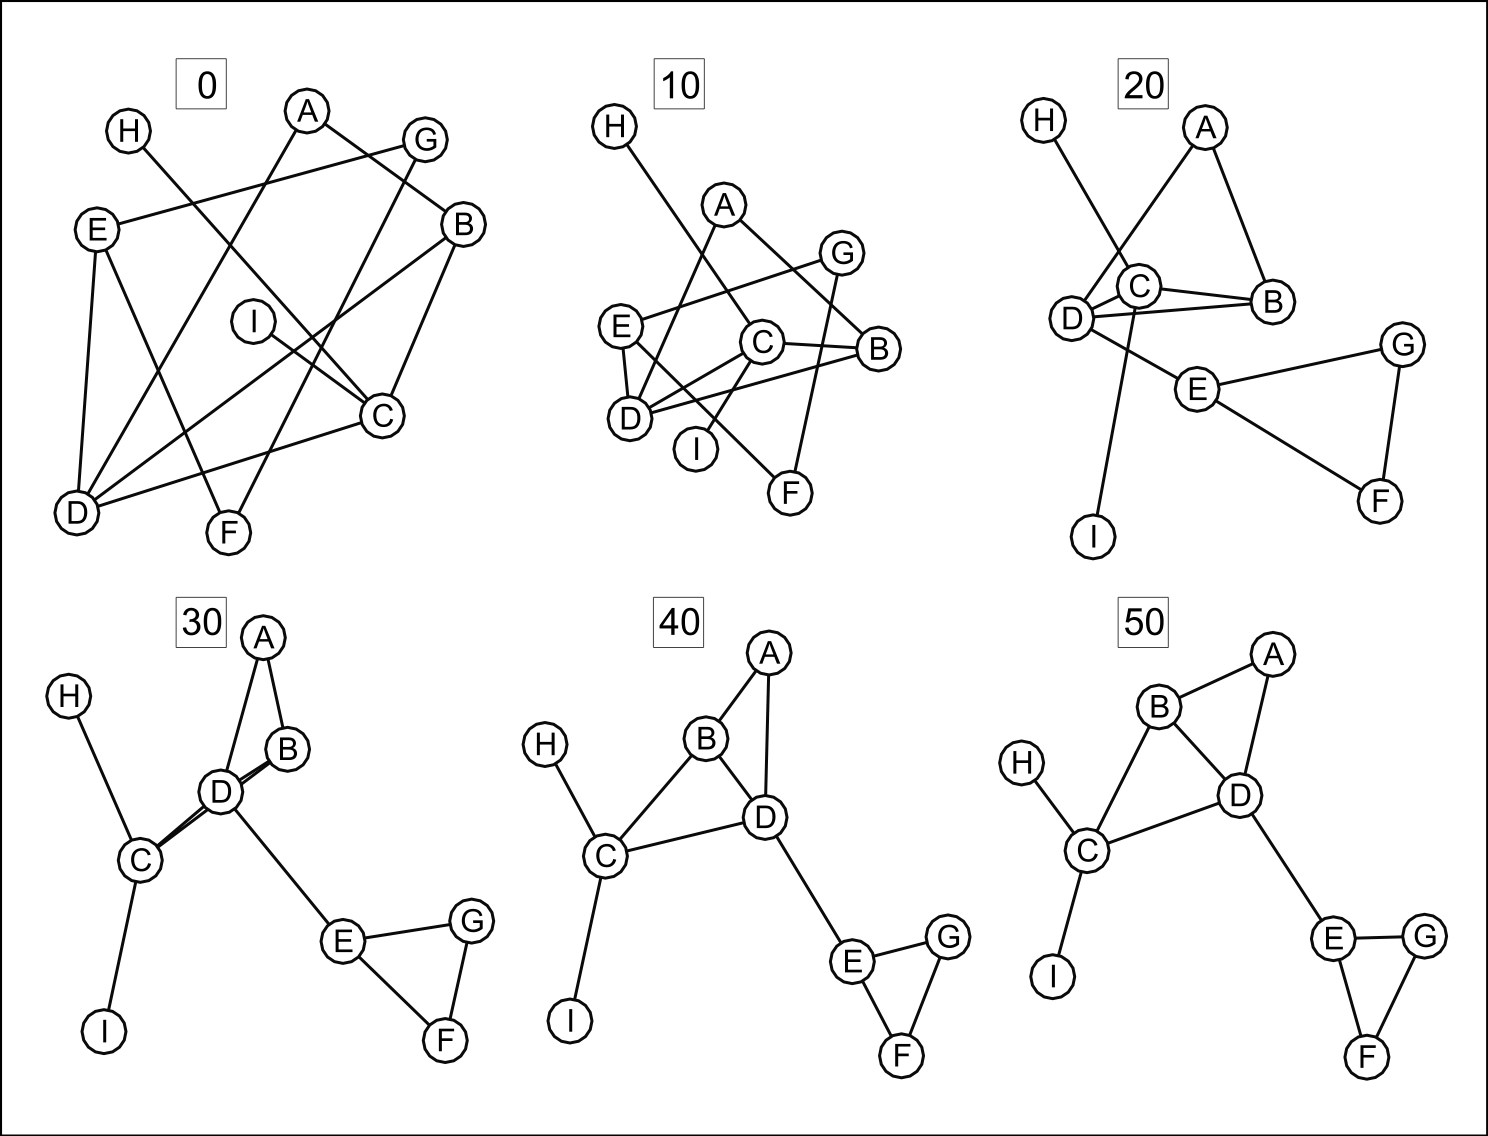
\includegraphics[width=\textwidth]{force-directed-layouts}
    \caption{Schrittweises Durchführen des Layout-Algorithmus von Fruchterman/Reingold}
    \bildquelle{Fruchterman, Thomas M. J./Reingold, Edward M.: Graph Drawing by Force-Directed Placement}
    \label{fig:force-directed-layouts}
\end{figure}

Force-Directed Layouts sind besonders effektiv für die übersichtliche
Darstellung von Netzwerken, in denen die Verbindungen zwischen den Elementen im
Vordergrund stehen. \parencite{schonfeld_fruchtermanreingold_2019} Im Gegensatz dazu
erfordert der Studiengangsfinder eine kontinuierliche Positionierung der
Studiengänge basierend auf inhaltlichen Ähnlichkeiten, was nicht unbedingt der
Stärke von Force-Directed Layouts entspricht. Force-Directed Graph Drawing
benötigt als Vorraussetzung bereits einen Graphen mit Knoten und Kanten, welche
im Fall des Studiengangsfinders die Ähnlichkeiten zwischen den einzelnen
Studiengängen entsprechen würde. Gerade die Berechnung der Ähnlichkeit zwischen
den einzelnen Studiengängen ist jedoch wesentlicher Bestandteil dieser Arbeit,
weshalb der Algorithmus nicht näher untersucht wurde.

\subsubsection{K-Means Clustering Algorithmus}
K-Means ist ein Clustering-Algorithmus, der Datenpunkte in $k$ vordefinierte
Gruppen oder Cluster einteilt. Die Wahl von $k$ stellt die Anzahl der Cluster dar,
und der Algorithmus versucht, die Datenpunkte so zu gruppieren, dass die Varianz
innerhalb der Cluster minimiert wird (siehe \autoref{fig:kmeans}).
\parencite{jeffares_k-means_2019}

\begin{figure}[H]
    \centering
    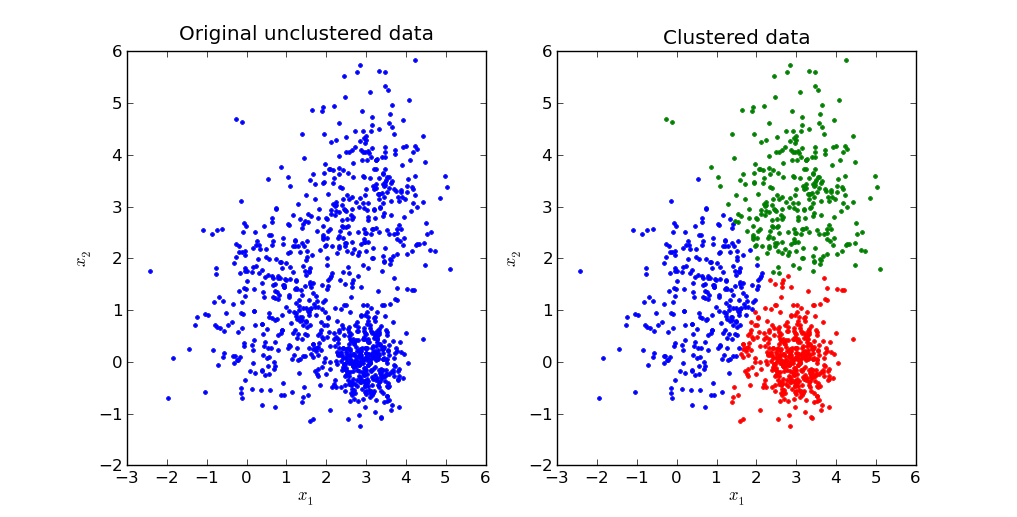
\includegraphics[width=\textwidth]{kmeans}
    \caption{K-Means Clustering Algorithmus}
    \bildquelle{https://mubaris.com/posts/kmeans-clustering/}
    \label{fig:kmeans}
\end{figure}

Die Entscheidung, den K-Means-Algorithmus nicht zu verwenden, basiert darauf, dass dieser hauptsächlich darauf abzielt, Datenpunkte zu gruppieren und weniger auf deren präzise Positionierung in einem zweidimensionalen Raum. Der Algorithmus fordert außerdem eine vordefinierte Clusteranzahl $k$. Das stellt im Falle des Studiengangsfinders jedoch keine Einschränkung dar, da jeder Cluster eine Inhaltskategorie, wie zum Beispiel \glqq Informatik\grqq{} repräsentieren würde. Dennoch ist der K-Means-Clustering-Algorithmus aufgrund seiner Empfindlichkeit gegenüber Ausreißern ungeeignet. Der Algorithmus versucht, Clusterzentren zu finden, die die Gesamtvarianz minimieren. Wenn es Ausreißer in den Studienschwerpunkten gibt, könnten sie das Ergebnis beeinflussen. \parencite{roth_demonstration_2023}

\subsubsection{Multidimensionale Skalierung (MDS)}\label{sec:MDS}
MDS ermöglicht die Reduktion $n$-dimensionaler Daten auf $m$-Dimensionen,
wodurch eine anschauliche Darstellung in Form von Koordinatenpaaren
ermöglicht wird \parencite{intro-to-multidimensional-scaling}. Dieser Aspekt ist
entscheidend, um Studiengänge in einem zweidimensionalen Diagramm zu
positionieren, wobei ähnliche Studiengänge aufgrund ihrer inhaltlichen
Ähnlichkeiten nahe beieinander liegen. Die Anwendung des MDS-Algorithmus auf
eine genormte Tabelle, in der im Falle von StudyMap die Studiengänge nach ihren
Anteilen an verschiedenen Inhaltskategorien gewichtet sind, ermöglicht eine
effektive Positionierung im Diagramm (siehe \autoref{table:input-mds}).

\begin{table}[!ht]
    \centering
    \begin{tabular}{|l|l|l|l|l|l|l|}
    \hline
        \textbf{Kürzel} & \textbf{Architektur} & \textbf{Gesundheit} & \textbf{Technik} & \textbf{Informatik} & \textbf{Wirtschaft} & \textbf{Internat.} \\ \hline
        \textbf{AT} & 0,55 & 0,06 & 0,09 & 0,04 & 0 & 0 \\ \hline
        \textbf{B} & 0,75 & 0 & 0 & 0,1 & 0 & 0,01 \\ \hline
        \textbf{ID} & 0,1 & 0,05 & 0,15 & 0,05 & 0,05 & 0 \\ \hline
        \textbf{HK} & 0,01 & 0,7 & 0,01 & 0,01 & 0,1 & 0,05 \\ \hline
        \textbf{PA} & 0 & 0 & 0,6 & 0,2 & 0,12 & 0,02 \\ \hline
        \textbf{IE} & 0 & 0 & 0,34 & 0,32 & 0,22 & 0,04 \\ \hline
        \textbf{LP} & 0 & 0,89 & 0,01 & 0 & 0,04 & 0,02 \\ \hline
        \textbf{SA} & 0 & 0,98 & 0 & 0 & 0 & 0 \\ \hline
        \textbf{IN} & 0 & 0 & 0,05 & 0,9 & 0 & 0,2 \\ \hline
        \textbf{IW} & 0 & 0 & 0,05 & 0,75 & 0,15 & 0,2 \\ \hline
        % \textbf{IM} & 0 & 0,2 & 0,1 & 0,65 & 0 & 0,05 \\ \hline
        % \textbf{BW} & 0 & 0 & 0 & 0 & 0,6 & 0,1 \\ \hline
        % \textbf{EB} & 0 & 0 & 0 & 0 & 0,5 & 0,4 \\ \hline
        % \textbf{SE} & 0 & 0 & 0,45 & 0,35 & 0,05 & 0,05 \\ \hline
        % \textbf{UI} & 0 & 0 & 0,36 & 0,12 & 0 & 0,04 \\ \hline
        % \textbf{MS} & 0 & 0 & 0,66 & 0,18 & 0 & 0,04 \\ \hline
        % \textbf{IR} & 0 & 0 & 0 & 0 & 0,1 & 0,8 \\ \hline
        % \textbf{REE} & 0 & 0 & 0,25 & 0,15 & 0,05 & 0,05 \\ \hline
        % \textbf{EI} & 0 & 0 & 0,5 & 0,25 & 0,05 & 0,05 \\ \hline
        % \textbf{ME} & 0 & 0 & 0,75 & 0,1 & 0,03 & 0,02 \\ \hline
        % \textbf{BE} & 0 & 0,07 & 0,6 & 0,12 & 0,11 & 0,06 \\ \hline
        % \textbf{MB} & 0 & 0 & 0,87 & 0,1 & 0,02 & 0 \\ \hline
        % \textbf{PT} & 0 & 0,95 & 0 & 0,03 & 0 & 0,09 \\ \hline
    \end{tabular}

    \caption{Exemplarische Eingabetabelle für den MDS-Algorithmus}
    \label{table:input-mds}
\end{table}

\autoref{table:input-mds} stellt eine stark vereinfachte Eingabetabelle für den
MDS-Algorithmus dar. Die erste Spalte enthält die Kürzel der verschiedenen
Studiengänge, wobei beispielsweise \textit{AT} für den Bachelor-Studiengang
Architektur steht. Die folgenden Spalten enthalten genormte Werte zwischen 0 und
1, die die prozentualen Anteile verschiedener Inhaltskategorien in den
jeweiligen Studiengängen repräsentieren. Diese genormten Werte werden im
n-dimensionalen Raum positioniert. Durch Anwendung des MDS-Algorithmus werden im
Verlauf die $n$-Dimensionen auf zwei Dimensionen reduziert, um schließlich eine
ästhetisch ansprechende Visualisierung in Form eines 2D-Diagramms zu generieren.

\noindent
Der klassische MDS-Algorithmus besteht aus den folgenden vier Schritten
\parencite{imperial_multidimensional_2019}:

% https://ceopedia.org/index.php/Multidimensional_scaling
\paragraph*{1. Berechnung der Distanzmatrix $ D_{ij} $}\label{sec:distanzmatrix}
Die Berechnung der Distanzmatrix $ D_{ij} $ erfolgt mithilfe des euklidischen
Abstands zwischen den Studiengängen im n-dimensionalen Raum. Der euklidische
Abstand zwischen zwei Punkten $ P_{i} $ und $ P_{j} $ wird nach der Formel

$$ d(P_i, P_j) = \sqrt{(x_i - x_j)^2 + (y_i - y_j)^2 + \ldots + (z_i - z_j)^2} $$

berechnet, wobei $ x_{i} $, $ y_{i} $, ..., $ z_{i} $ die Koordinaten von Punkt
$ P_{i} $ im $n$-dimensionalen Raum sind \parencite{ceopedia_multidimensional_2018}. Für die
Studiengangsdaten bedeutet das, dass die $n$-Dimensionen die verschiedenen
Inhaltskategorien repräsentieren.

Die euklidische Distanzmatrix $ D_{ij} $ enthält dann die euklidischen Abstände
zwischen jedem Paar von Studiengängen. In der Matrix sind die Elemente
$ D_{ij} $ die Distanzen zwischen den Studiengängen $ i $ und $ j $. Je näher
die Studiengänge in der Distanzmatrix beieinander liegen, desto näher werden sie
im finalen Diagramm platziert und umgekehrt.

Konkret in Python implementiert, sieht die Berechnung der Distanzmatrix wie
folgt aus:

\begin{lstlisting}[style=Python]
def calculate_distance_matrix(X):
    euclidean = lambda x,y:ma.sqrt(np.sum((np.array(x)-np.array(y))**2))
    D = []
    for x in X:
        tmp = []
        for y in X:
            tmp.append(euclidean(x, y))
        D.append(tmp)
    return D
\end{lstlisting}

% https://dorianhe.github.io/Intro-to-Multidimensional-Scaling/
% https://ceopedia.org/index.php/Multidimensional_scaling
% https://www.hongfeili.com/files/paper100/paper4.pdf
\paragraph*{2. Anwendung der Centering Matrix $ C $ zur Normalisierung der
Distanzen}
Die Formel $ C = I - \frac{1}{n} \vec{e} * \vec{e}^T $ berechnet die sogenannte Centering Matrix. $ I $ ist die Einheitsmatrix, $ \frac{1}{n} $ ist der Kehrwert der Anzahl der Datenpunkte und $ \vec{e} $ ist ein Vektor gefüllt mit Einsen. Das Symbol $ \vec{e}^T $ bezeichnet wie in der Mathematik üblich die Transposition des Vektors. \parencite{wickelmaier_introduction_2003}

Die Centering Matrix $ C $ wird verwendet, um die Distanzmatrix $ D $ zu
zentrieren. Das Zentrieren ist wichtig, um die Distanzen zwischen den Punkten
in der $n$-dimensionalen Raummatrix zu normieren und somit den Schwerpunkt der
Daten im Raum zu korrigieren. \parencite{wickelmaier_introduction_2003}

Schließlich wird diese eingesetzt um die Zentriermatrix $ B $ aus der
Distanzmatrix zu berechnen:
$$ B = - \frac{1}{2} * C * D_{ij} * C $$

\paragraph*{3. Spektralzerlegung}
Die Matrix $ B $ wird nun spektral zerlegt, um die Eigenwerte $ \lambda_{i} $
und die zugehörigen Eigenvektoren $ v_{i} $ zu erhalten.
$$ B = W * \Lambda * W^-1 $$
Hierbei ist $ W $ die Matrix der Eigenvektoren und $ \Lambda $ ist eine
Diagonalmatrix mit den Eigenwerten auf der Hauptdiagonale. Die Eigenvektoren
werden anschließend sortiert und die größten positiven Eigenwerte
$ \lambda_{1} ... \lambda{m} $ mit dazugehörigen Eigenvektoren
$ v_{1} ... v_{m} $ aus B extrahiert. \parencite{wickelmaier_introduction_2003}

\paragraph*{4. Projektion der Datenpunkte}
Um nun die Datenpunkte von einem höherdimensionalen Raum (basierend auf den
Beziehungen in der Distanzmatrix $ D $) auf einen niedrigdimensionalen Raum,
der durch die Eigenvektoren und Eigenwerte repräsentiert wird, abzubilden,
benötigt man folgende Projektion \parencite{he_classical_2018}:
$$ X = V_m \Lambda^{1/2}_m $$
Die Variable $ m $ steht für die Anzahl der gewünschten Dimensionen. Im Falle
von StudyMap entspricht $ m = 2 $, um das Ergebnis in einem 2D-Diagramm zu
visualisieren. $ V_{m} $ steht für die Eigenvektoren und $ \Lambda $ wie bereits
im vorherigen Absatz beschrieben für die Diagonalmatrix mit den Eigenwerten.
\parencite{wickelmaier_introduction_2003}

Abschließend enthält $ X $ die Matrix mit den auf $ m $-Dimensionen reduzierten
Koordinaten, welche dann z.B. in einem Diagramm visualisiert werden können.
An dieser Stelle wird für die Berechnung der Studiengänge (mit $ m = 2 $)
ermöglicht, dass innerhalb einer 2D-Darstellung, ähnliche Studiengänge aufgrund
ihrer inhaltlichen Ähnlichkeiten nahe beinander positioniert werden. Diese
räumliche Anordnung erleichtert die intuitive Analyse von Beziehungen zwischen
den einzelnen Bachelor- und Masterstudiengängen.

Insgesamt erfüllt der MDS-Algorithmus die spezifischen Anforderungen des
Studiengangsfinders, indem er eine übersichtliche und interpretierbare
Visualisierung der Studiengänge basierend auf inhaltlichen Ähnlichkeiten
ermöglicht.

\subsection{Beschreibung der Datenquelle und -beschaffung}
\subsubsection{Herkunft der Daten}\label{sec:herkunft-der-daten}
Die Grundlage für den Studiengangsfinder wurde in enger Zusammenarbeit mit Frau
Rösel, der Vizepräsidentin der Hochschule Regensburg, gelegt. Wir initiierten
den Prozess durch die Definition klarer Anforderungen an die benötigten
Informationen. Dazu gehört unter anderem die Definition der Inhaltskategorien
der Studiengänge. Der erste Entwurf entsprach folgender Aufteilung:

\begin{enumerate}
    \item Architektur und Bau
    \item Design und Medien
    \item Gesundheit und Soziales
    \item Technik
    \item Informatik und Mathematik
    \item Marketing und Kommunikation
    \item Erneuerbare Energien, Nachhaltigkeit und Umwelttechnik
    \item Wirtschaft und Management
    \item Internationales
\end{enumerate}

Diese Anforderungen wurden dann innerhalb der Hochschule kommuniziert und von
einer Teilmenge der Studiendekane für vereinzelte Studiengänge ausgefüllt. Das
heißt konkret, dass für 22 Studiengänge jeweils für alle dieser
Inhaltskategorien ein Wert festgelegt wurde.

Frau Rösel bleibt bis zur Übergabe der Arbeit weiterhin für die Beschaffung der Daten verantwortlich. Eine systematische Bewertung aller Studiengänge anhand des Modulplans und der jeweiligen ECTS pro Inhaltskategorie wird von Frau Rösel in Zusammenarbeit mit den Studiengangsverantwortlichen entwickelt.

Das European Credit Transfer System (ECTS) ist ein System zur Normierung von Studienleistungen innerhalb des Europäischen Hochschulraums. Dadurch können Unterschiede zwischen nationalen Hochschulsystemen ausgeglichen werden. \parencite{european_commission_europaisches_nodate} Jedes Fach an der OTH Regensburg hat eine bestimmte Anzahl von Credits (ECTS), die sich nach der Intensität des Faches richtet.

Die Bewertung des Studiengangsfinders erfolgt auf Basis der Inhaltskategorien und wird nun neutral nach der ECTS-Anzahl der jeweiligen Kategorie berechnet. So wird eine objektive Einstufung der Studiengänge für den verwendeten MDS-Algorithmus gewährleistet. Durch objektive Berechnungen ist es in Zukunft denkbar, die Aufgabe der Datenaktualisierung an eine dritte Person zu delegieren.

\subsubsection{Festlegung der Inhaltskategorien}
Im nächsten Schritt werden die Werte auf die Zeile normiert. Das heißt, die
Summe aller Inhaltskategorie-Werte pro Studiengang beträgt eins.

Im Umkehrschluss bedeutet das jedoch, dass die Studiengänge aufgrund von
Überschneidungen in den Kategorien nicht korrekt abgebildet werden können.
Beispiel:

\begin{table}[!ht]
    \centering
    \begin{tabular}{|l|l|l|l|l|}
    \hline
    \textbf{Studienfeld}           & \textbf{...} & \textbf{Informatik und Mathematik} & \textbf{Internationales} & \textbf{...} \\ \hline
    Informatik                     & ...          & 0,8                                & 0,2                      & ...          \\ \hline
    International Computer Science & ...          & 0,4                                & 0,6                      & ...          \\ \hline
    \end{tabular}

    \caption{Aufteilung der Werte bei auf Studiengang genormte Werte}
    \label{table:norm-values}
\end{table}

Tabelle \ref{table:norm-values} zeigt die Problematik der Überschneidungen. Der
Studiengang International Computer Science ist von den Inhalten nahezu
identisch zum Studiengang Informatik. Der Hauptunterschied ist, dass die Fächer
in Englisch angeboten werden. Dies hat zur Folge, dass der Studiengang
eigentlich sowohl in der Kategorie Informatik und Mathematik, als auch in der
Kategorie Internationales einen hohen Wert benötigt. Da die Zeilensumme eins
beträgt, ist dies nicht realistisch abbildbar. Aus diesem Grund wurde
entschieden die Werte pro Zelle, d.h. pro Kategorie und Studiengang auf eins
zu normieren. Mit dieser Aufteilung, kann ein Studiengang sowohl in Informatik
und Mathematik beispielsweise einen Wert von 0,8 haben, als auch in der
Kategorie Internationales.

Die anfängliche Kategorisierung der Studiengänge in neun allgemeine
Inhaltskategorien stellte sich als unzureichend heraus, da nach der Anwendung
des MDS-Algorithmus viele Studiengänge überlappend dargestellt wurden. Diese
Herausforderung führte zu einer entscheidenden Überarbeitung des
Kategorisierungssystems, um präzisere und differenzierte Bewertungen zu
ermöglichen. Die Lösung bestand in der Einführung von sogenannten Supergruppen,
die eine tiefere Bewertung der Studiengänge ermöglichten.

Ursprünglich waren Studiengänge wie \textit{Architektur} und
\textit{Bauingenieurwesen} in einer einzigen Kategorie
\textit{Architektur und Bau} zusammengefasst. Die Neuerung bestand darin, diese
in separate Kategorien wie \textit{Architektur} und \textit{Bau} zu unterteilen.
Ein zusätzliches Feld in der Eingabedatei legte fest, welche dieser Kategorien
später in der Benutzeroberfläche zu einer Supergruppe zusammengeführt werden
sollten. Dieser Ansatz ermöglichte eine präzisere Bewertung von Studiengängen,
insbesondere bei Studiengängen wie \textit{Architektur} und
\textit{Bauingenieurwesen}. Hier konnte der Studiengang \textit{Architektur} als
mehr \textit{Architektur} und weniger \textit{Bau} bewertet werden, während es
bei \textit{Bauingenieurwesen} genau umgekehrt war. Vor dieser Anpassung konnte
nur ein Wert für \textit{Architektur und Bau} festgelegt werden.

Um die Benutzeroberfläche übersichtlich zu halten, wurden Supergruppen
eingeführt. Diese ermöglichen eine aggregierte Darstellung mehrerer Kategorien,
ohne die Benutzeroberfläche unnötig zu komplex zu gestalten. Frau Rösel brachte
entscheidende Impulse in diesen Prozess ein. Durch ihre Rückmeldung wurden
darüber hinaus neue Kategorien wie \textit{Sprachkompetenzen},
\textit{Digitalität} und \textit{Future Skills} eingeführt. Diese dienen dazu,
eine noch präzisere Differenzierung und Bewertung der Studiengänge zu
ermöglichen. Folgende Liste zeigt die neuen Kategorien - jeder Listeneintrag
enthält dabei eine Supergruppe mit einem oder mehrere Kategorien:

\begin{enumerate}
    \item Architektur, Bau (Architektur und Bau)
    \item Design, Medien (Design und Medien)
    \item Gesundheit, Soziales (Gesundheit und Soziales)
    \item Maschinenbau, Elektrotechnik (Technik)
    \item Informatik (Informatik)
    \item Naturwissenschaften, Mathematik (Naturwissenschaften und Mathematik)
    \item Marketing, Kommunikation (Marketing und Kommunikation)
    \item Erneuerbare Energien, Umwelttechnik (Erneuerbare Energien und
    Umwelttechnik)
    \item Nachhaltikeit (Nachhaltigkeit)
    \item Wirtschaft, Management (Wirtschaft und Management)
    \item Sprachkompetenzen (Sprachkompetenzen)
    \item Digitalität (Digitalität)
    \item Future Skills (Future Skills)
\end{enumerate}

Die neuen Kategorien, ergänzt durch die Einführung der Supergruppen, schaffen
eine optimierte Grundlage für den MDS-Algorithmus. Dieser kann nun Studiengänge
präziser positionieren, da die Unterscheidungen und Bewertungen auf einer
feineren Ebene vorgenommen werden. Diese Anpassungen tragen entscheidend dazu
bei, das Ziel einer verfeinerten Studienorientierung und -wahl zu erreichen.
\newpage

% Konzept und Umsetzung an der OTH-Regensburg
\section{Konzept und Umsetzung an der OTH-Regensburg}

\subsection{Vorstellung der OTH-Regensburg als Fallbeispiel}

\subsection{Konzept für eine automatisch generierte Infografik}

\subsection{User-centered Design Research: Mockup eines Prototypen}

\subsection{Beschreibung der Positionsberechnung der Infografik}

\subsection{Technische Details zur Umsetzung}

\subsection{Anwendung des entwickelten Systems auf die Studiengänge der OTH-Regensburg}
\newpage

% Mockup-, und Prototypen-Studie
\section{User-centered Design Research}

\subsection{Mockup-Studie: Bewertung der Benutzerfreundlichkeit und
Funktionalität}
Bei der Entwicklung eines nutzerzentrierten Designs steht die direkte Einbindung
der Zielgruppe im Mittelpunkt. Dieser Ansatz, der als User-Centered Design (UCD) 
bezeichnet wird, stellt die Integration der Bedürfnisse, Erwartungen und
Anforderungen der Benutzer in den Entwicklungsprozess in den Mittelpunkt. Ziel
ist es, Produkte und Anwendungen zu gestalten, die nicht nur funktional und
ästhetisch ansprechend sind, sondern auch die bestmögliche
Benutzerfreundlichkeit bieten.

\subsubsection{Methodik und Teilnehmende}
Im Rahmen des UCD-Prozesses wurde das zuvor in Kapitel \ref{sec:konzept}
vorgestellte Mockup-Konzept für den Studiengangsfinder entwickelt, das als
Prototyp diente. Um sicherzustellen, dass das entworfene Konzept den
Bedürfnissen der potenziellen Nutzer entspricht, wurde eine gezielte 
User-Centered-Design-Studie durchgeführt. Zu diesem Zweck wurden sechs
Studierende und Absolventen verschiedener Fachrichtungen eingeladen, den
Mockup-Entwurf zu evaluieren (siehe \autoref{table:teilnehmer-mockup-studie}).

\begin{table}[!ht]
    \centering
    \begin{tabular}{|l|l|l|l|}
        \hline
        \textbf{\#} & \textbf{Studienabschluss}                               & \textbf{Geschlecht} & \textbf{Datum} \\ \hline
        1           & Betriebswirtschaft B.A.                                 & Weiblich            & 16.09.2023     \\ \hline
        2           & Psychologie M.Sc.                                       & Weiblich            & 20.09.2023     \\ \hline
        3           & Informatik B.Sc.                                        & Männlich            & 25.09.2023     \\ \hline
        4           & Regenerative Energietechnik und Energieeffizienz B.Eng. & Männlich            & 07.10.2023     \\ \hline
        5           & Bioprozessinformatik B.Sc.                              & Männlich            & 08.10.2023     \\ \hline
        6           & Betriebswirtschaft B.A.                                 & Weiblich            & 12.10.2023     \\ \hline
    \end{tabular}

    \caption{Probanden der Mockup-Studie}
    \label{table:teilnehmer-mockup-studie}
\end{table}

\subsubsection{Ablauf des Tests}
Die Studie wurde in Form von Einzelinterviews durchgeführt. Die Teilnehmer wurden ermutigt, ihre persönlichen Perspektiven, Erfahrungen und Vorschläge einzubringen. Außerdem wurden sie gebeten, ihre Gedanken zum Entwurf laut zu äußern. Anschließend wurden ihnen nacheinander alle Grafiken des Entwurfs gezeigt (1. \autoref{fig:mockup-bubbles},
2. \autoref{fig:mockup-bubbles-hover}, 3. \autoref{fig:mockup-bubbles-popup}). 

Offene Fragen zu Designelementen, Verständlichkeit von Informationen und allgemeinen Nutzererfahrungen sollten Aufschluss über mögliche Stärken und Schwächen des Design-Proto\-typs geben. Ziel war es, frühzeitig wertvolles Feedback zu erhalten, um Optimierungen und Anpassungen vornehmen zu können, bevor die Umsetzung in die nächste Phase geht. Die lauten Gedanken der Teilnehmerinnen und Teilnehmer wurden von Herrn Huber in einem Freitextfeld dokumentiert.

\subsubsection{Ergebnisse der Mockup-Studie}
Die Rückmeldungen der Studienteilnehmenden lassen sich in folgende konsistente
Muster zusammenfassen.

\paragraph{Bild 1: Visualisierung der Studiengänge}\label{sec:visualisierung-der-studiengänge}
Die Übersichtskarte wurde von den Teilnehmenden als unübersichtlich und geclustert wahrgenommen. Besonders die Farbähnlichkeit der Studiengänge wurde als störend
empfunden.

Eine konkrete Verbesserungsmöglichkeit besteht darin, die Überschriften der Nebel zu vergrößern und fett darzustellen, um die Lesbarkeit zu verbessern. Darüber hinaus wurde vorgeschlagen, alle Abkürzungen der Studiengänge standardmäßig auszublenden und nur den Nebel zu beschriften, um die Übersichtlichkeit zu erhöhen. Sobald der Benutzer mit der Maus in die Nähe des Nebels kommt, sollte die Überschrift des Nebels ausgeblendet und die Abkürzungen aller darin enthaltenen Studiengänge eingeblendet werden. Um die Zufälligkeit und Ähnlichkeit der Farben zu vermeiden, könnten die Studiengänge in den Fakultätsfarben und der Nebel im Hintergrund neutral (z.B. grau) eingefärbt werden.

\paragraph{Bild 2: Interaktivität}
Das Hover-Event über eine Bubble mit einem Tooltip wurde durchweg als passend und verständlich betrachtet. Dieses Element wurde von den Teilnehmenden als intuitiv und funktional empfunden.

\paragraph{Bild 3: Popup mit Details eines Studiengangs}
Über die Anordnung der Informationen im Popup gingen die Meinungen auseinander. Während einige eine absteigende Sortierung nach Relevanz bevorzugten, sprachen sich andere für eine alphabetische Sortierung aus. Positiv bewertet wurde die Funktion, ähnliche Studiengänge nach Ähnlichkeit zu sortieren. Die Darstellung der Branchen wurde als weniger aussagekräftig empfunden und teilweise vorgeschlagen, diese Information zu entfernen. Die Möglichkeit, sich Unternehmen in Regensburg anzeigen zu lassen, wurde positiv bewertet und es wurde angeregt, diese Funktion ausklappbar zu gestalten, um die Übersichtlichkeit zu erhöhen. Es wurde außerdem empfohlen, die Informationen zu den Einstiegsgehältern zu erläutern, möglicherweise durch die Integration von Fragezeichensymbolen und Tooltips.

\paragraph{Generelle Anmerkungen}
Zu den allgemeinen Verbesserungsvorschlägen gehören ein besserer Farbkontrast, mehr Erläuterungen zu verschiedenen Informationen und eine einheitliche und intuitive Anordnung der Designelemente, um die Übersichtlichkeit insgesamt zu erhöhen.

%
%
%
%
%
%
% PROTOTYPEN STUDIE
\subsection{Prototypen-Studie: Evaluation durch Studieninteressierte}
Nach der Entwicklung des Prototyps auf Basis des Mockups und der Erkenntnisse aus der Mockup-Studie wurden Studieninteressierte eingeladen, den Prototyp von StudyMap zu testen. Nach der selbstständigen Interaktion mit dem Prototyp wurden die Teilnehmenden gebeten, an einer Umfrage teilzunehmen, um ihre Erfahrungen, Meinungen und Verbesserungsvorschläge zu dokumentieren.

Der folgende Abschnitt beleuchtet die Methodik, den genauen Ablauf des Tests und stellt die Ergebnisse dieser Evaluationsstudie vor, die wertvolle Einblicke in die Effektivität und Benutzerfreundlichkeit des Prototyps liefert.

\subsubsection{Methodik und Teilnehmende}
Der nächste Schritt im UCD-Prozess ist das Testen des Prototyps mit potenziellen Nutzern, d.h. Studieninteressierten. Zu diesem Zweck wurde auf der Grundlage des Mockups und der im vorherigen Kapitel beschriebenen Mockup-Studie ein Prototyp entwickelt (siehe \autoref{fig:prototyp-overview}). Ziel dieser Studie ist es, frühe Designentscheidungen zu hinterfragen und das Tool auf Usability zu testen. Der Vorteil einer solch frühen Evaluierung ist, dass größere Änderungen am Endprodukt wesentlich aufwendiger sind als in einem frühen Entwicklungsstadium.

\begin{figure}[H]
    \centering
    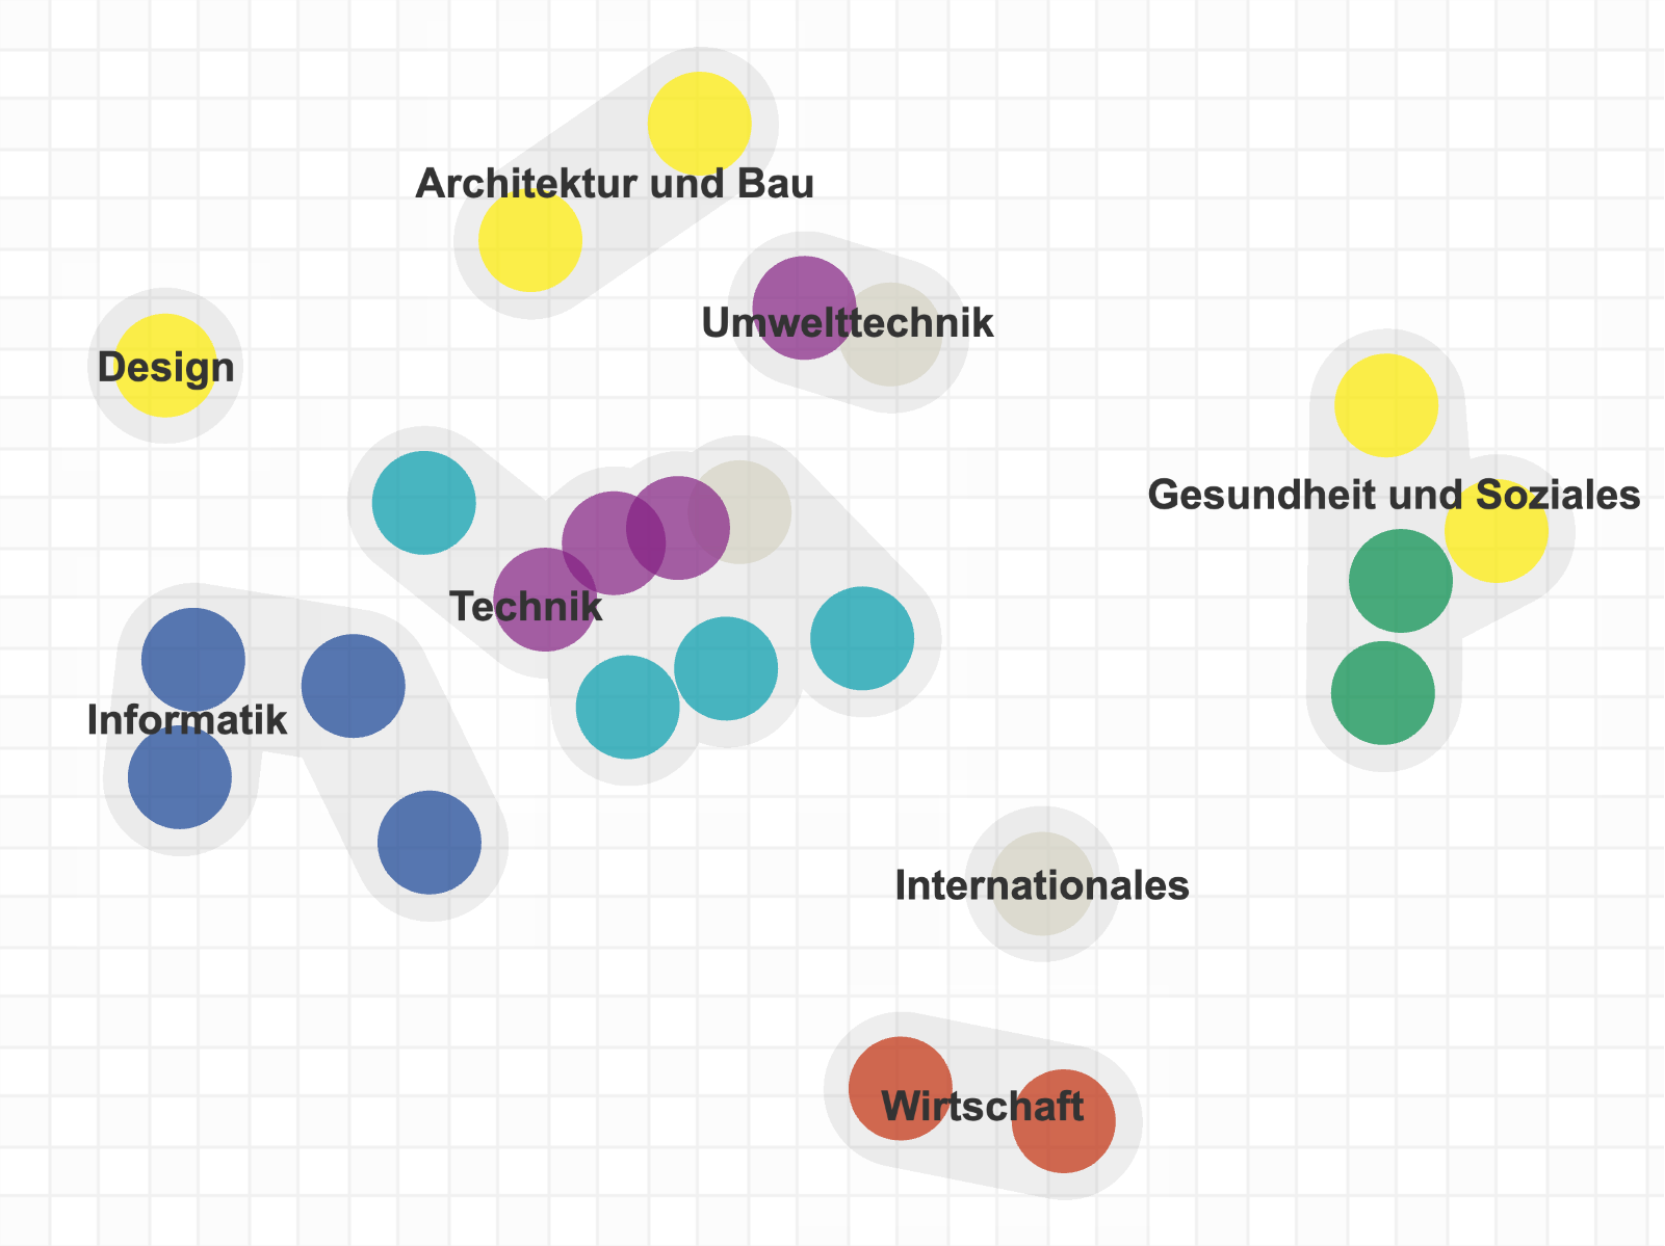
\includegraphics[width=\textwidth]{prototyp_overview}
    \caption{StudyMap Prototyp}
    \bildquelle{Eigene Darstellung}
    \label{fig:prototyp-overview}
\end{figure}

An der Studie nahmen 40 Schülerinnen und Schüler der 11. Klasse des Johannes-Nepomuk-Gymnasiums in Rohr i.NB teil. Alle diese Schüler werden voraussichtlich im Jahr 2026 die allgemeine Hochschulreife erlangen und entsprechen damit genau der Zielgruppe eines Studiengangfinders. Durch die örtliche Nähe des Gymnasiums zur OTH-Regensburg ist die Eignung des Teilnehmerkreises zusätzlich gegeben.

Die Befragung fand in zwei Gruppen (Klasse 11A und Klasse 11B) im Johannes-Neopomuk-Gymnasium vor Ort im Computerraum der Schule statt. Dort konnten die Schülerinnen und Schüler an den Windows-Rechnern der Schule sowohl den Prototyp testen als auch die Umfrage in Einzelarbeit beantworten.

\subsubsection{Ablauf des Tests}
Die Studie begann mit einer kurzen Einführung, in der den Teilnehmenden der
Zweck der Studie und die Handhabung des Prototyps erläutert wurden. Anschließend
wurden die Teilnehmenden gebeten, den Prototyp selbst zu verwenden und zwei
Aufgaben innerhalb einer Online-Umfrage zu lösen, um die Benutzerfreundlichkeit, die Navigationsstruktur und
die Funktionalitäten des Studiengangsfinders zu testen (siehe
\autoref{fig:prototyp-umfrage-aufgaben} - \textbf{Umfrage Teil 2}). In dieser Phase wurden sowohl
quantitative als auch qualitative Daten erhoben, um ein umfassendes Bild der 
Benutzererfahrung zu erhalten.

\begin{figure}[H]
    \centering
    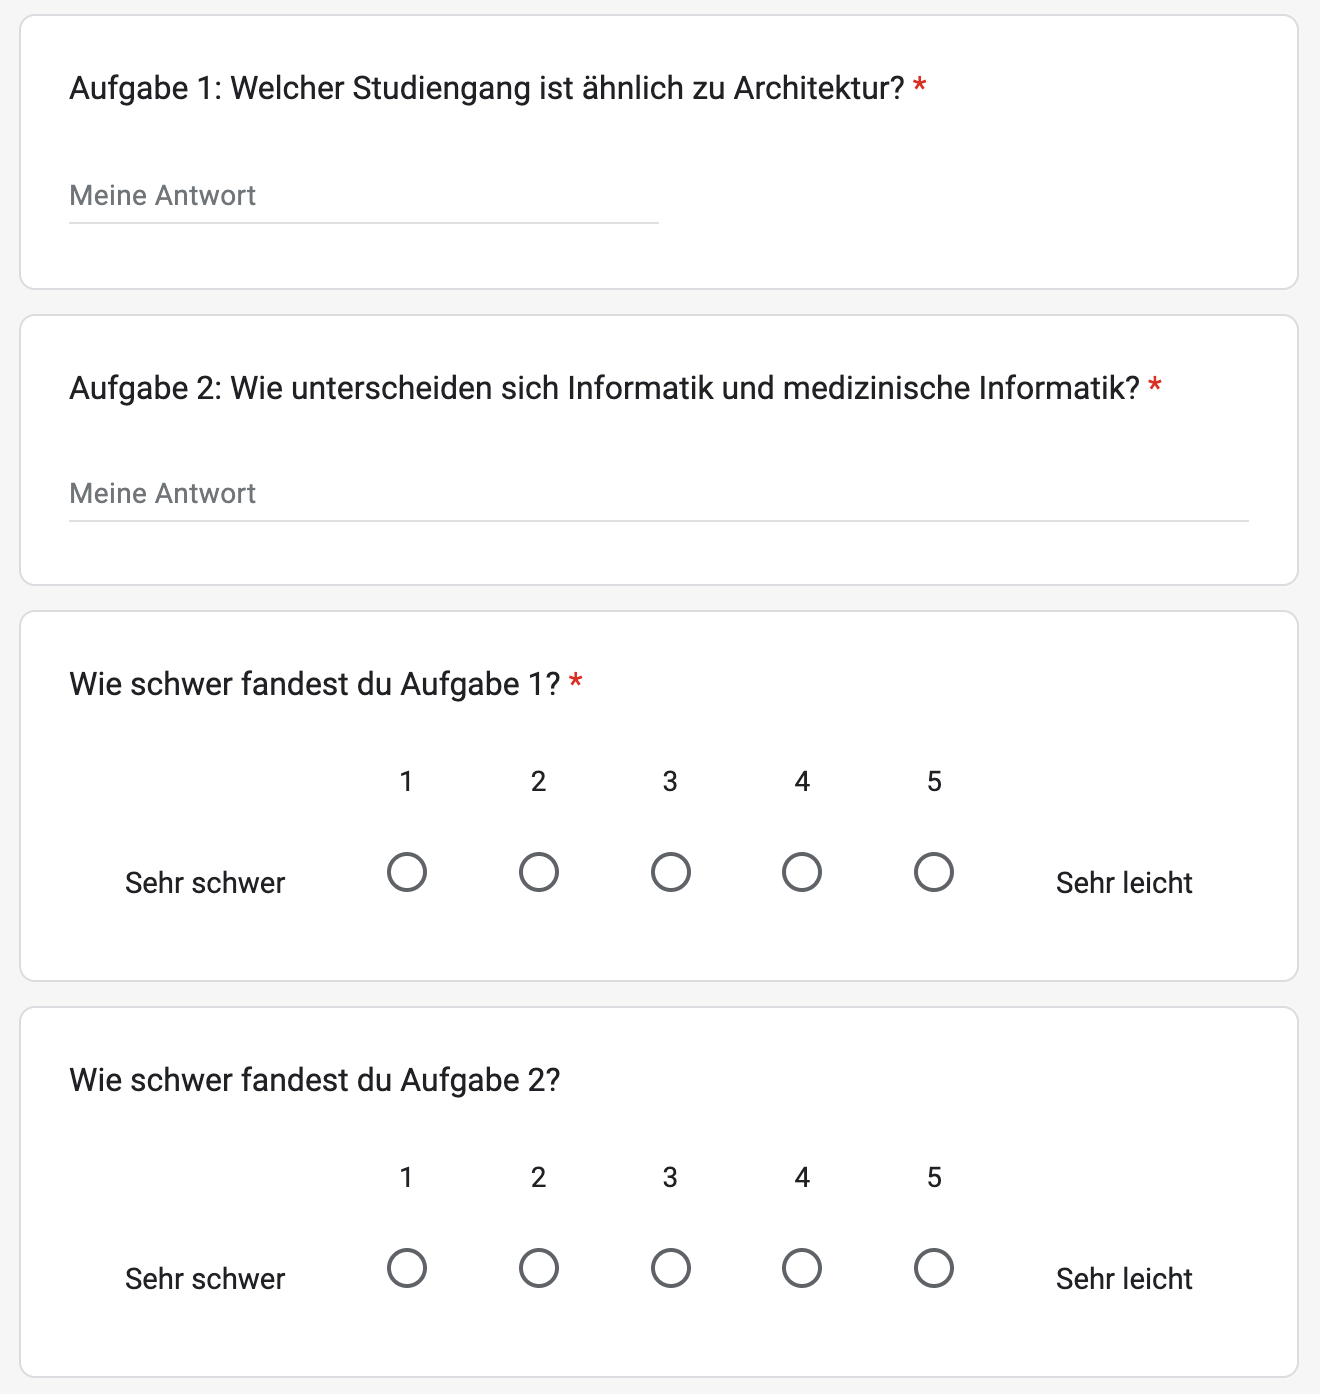
\includegraphics[width=0.5\textwidth]{umfrage_aufgaben}
    \caption{Prototypen-Studie: Aufgaben (Umfrage Teil 2)}
    \bildquelle{Eigene Darstellung}
    \label{fig:prototyp-umfrage-aufgaben}
\end{figure}

Nach der Interaktion mit dem Prototyp wurden die Teilnehmenden gebeten, zusätzlich zu den Aufgaben weitere Fragen in der anonymen Online-Umfrage zu beantworten.

Die ersten Fragen der Umfrage waren Multiple-Choice-Fragen mit den Antwortmöglichkeiten \glqq Ja\grqq{}, \glqq Nein\grqq{} und \glqq Keine Angabe\grqq{} \textbf{(Umfrage Teil 1)}.

\begin{enumerate}
    \item Willst du nach dem Abi studieren?
    \item Wenn ja, weißt du schon, was für ein Studium?
    \item Würde dir StudyMap bei der Wahl des Studiengangs helfen?
    \item Die Antwort hier ist \glqq Ja\grqq{} (Aufmerksamkeitsfrage)
\end{enumerate}

Danach folgten die beiden oben beschriebenen Aufgaben (siehe
\autoref{fig:prototyp-umfrage-aufgaben}). Zuletzt wurden die folgenden Fragen
mit Freitextfeldern zur Beantwortung gestellt \textbf{(Umfrage Teil 3)}:

\begin{enumerate}
    \item Was findest du an dem Konzept gut?
    \item Was findest du am Konzept schlecht?
    \item Hast du neue Ideen für den Prototyp?
    \item Wenn du bei \glqq Würde StudyMap dir bei der Studienwahl helfen?\grqq{} NEIN angekreuzt hast: Warum nicht?
\end{enumerate}

Die Fragen wurden bewusst mit Freitextfeldern zur Beantwortung versehen, um den Teilnehmenden die Möglichkeit zu geben, mit allen möglichen Gedankengängen zu antworten. Dies kann dazu führen, dass Ideen entstehen, die bisher noch nicht bedacht wurden und somit im Endprodukt umgesetzt werden können. Die Befragung dauerte ca. 15 Minuten. Durch die Kombination der Interaktion mit dem Prototyp und der schriftlichen Befragung konnten vielfältige Einblicke in die Nutzerperspektive gewonnen werden.

\subsubsection{Ergebnisse der Prototypen-Studie}

\paragraph{Umfrage Teil 1: Fragen}

\begin{figure}[H]
    \centering
    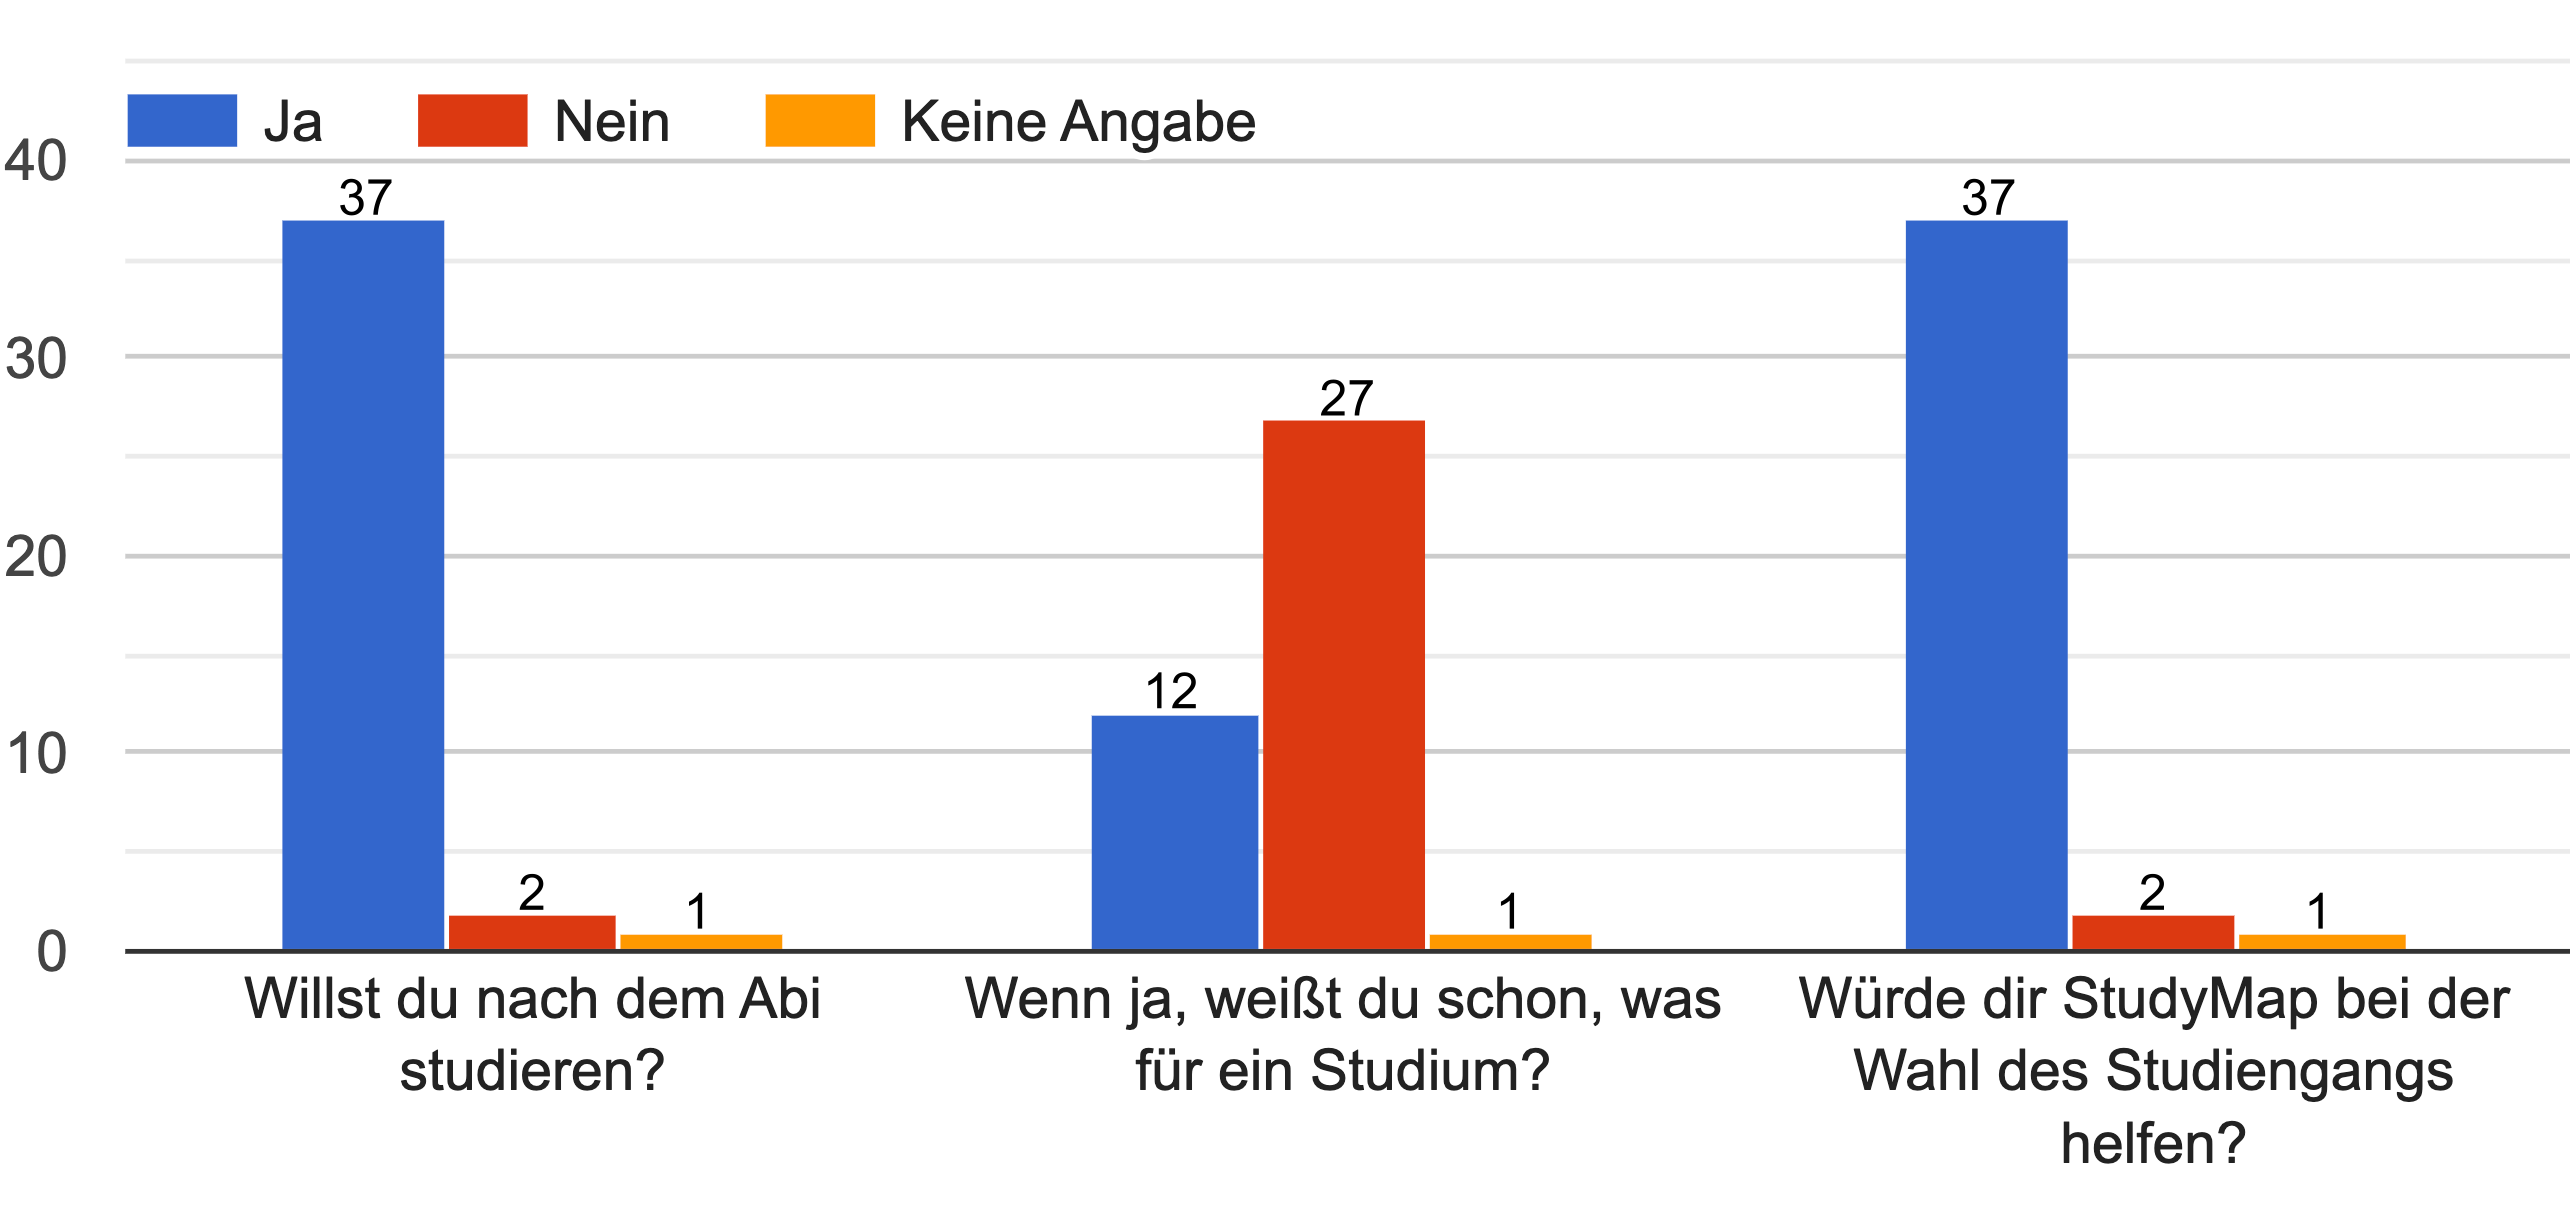
\includegraphics[width=\textwidth]{linien_fragen_1}
    \caption{Ergebnisse: Teil 1}
    \bildquelle{Google Forms + selbst ergänzte absolute Werte}
    \label{fig:linien-fragen-1}
\end{figure}

\autoref{fig:linien-fragen-1} zeigt, dass die erste Frage (\glqq Möchtest du nach dem Abitur studieren?\grqq{}) von 92,5 \% der Befragten bejaht wurde. Während zwei Personen (5 \%) die Frage verneinten, machte nur eine Person (2,5 \%) keine Angabe. Daraus lässt sich schließen, dass es sich bei der gewählten Teilnehmergruppe tatsächlich um die richtige Zielgruppe von StudyMap handelt.

Auf die Frage \glqq Wenn ja, weißt du schon, was du studieren willst?\grqq{} antworteten 30 \% (12) der Befragten mit \glqq Ja\grqq{}. 67,5 \% (27) haben mit \glqq Nein\grqq{} geantwortet und 2,5 \% haben wiederum die Angabe verweigert. Die Person, die bei Frage 1 angegeben hat, nicht zu antworten, hat bei dieser Frage mit \glqq Nein\grqq{} geantwortet. Die Person, die bei Frage 2 mit \glqq Keine Angabe\grqq{} stimmte, hatte zuvor bei Frage 1 mit \glqq Ja\grqq{} gestimmt. Die beiden Schüler, die bei Frage 1 mit \glqq Nein\grqq{} für ein Studium geantwortet haben, haben auch Frage 2 mit \glqq Nein\grqq{} votiert.

Zieht man die beiden Schülerinnen und Schüler, die sich bei Frage 1 gegen ein Studium entschieden haben, von den \glqq Nein\grqq{}-Antworten bei Frage 2 ab, so verbleiben 25 von 37 Studieninteressierten, die noch nicht wissen, was sie studieren werden. Daraus ergibt sich ein Anteil von 67,57 \% der Schüler der 11. Klasse, welche voraussichtlich nach dem Abitur eine Studienorientierung benötigen. Dieser Anteil an Schülern könnte mithilfe des innovativen Studiengangsfinders zu einem passenden Studiengang geführt werden.

Die dritte Frage (\glqq Würde dir StudyMap bei der Studienwahl helfen?\grqq{}) wurde von 37 von 40 Teilnehmern (92,5 \%) bejaht. Zwei Teilnehmer antworteten mit \glqq Nein\grqq{} und eine Person enthielt sich der Stimme. Im Falle einer Verneinung hatten die Befragten die Möglichkeit, dies im Anschluss in einem Freitextfeld zu begründen. Die beiden Personen, die mit \glqq Nein\grqq{} geantwortet haben, gaben an, dass StudyMap ihnen nicht bei der Studienwahl helfen würde, da sie bereits wüssten, was sie studieren wollen. Die Antworten auf diese Frage verdeutlichen noch einmal den Bedarf des Studiengangsfinders als Orientierungshilfe für Studieninteressierte.

Die Frage Nr. 4 der Umfrage Teil 1 wurde von allen Teilnehmern korrekt mit \glqq Ja\grqq{} beantwortet. Sie diente dazu, willkürlich ausgefüllte und damit nicht auswertbare Teilnahmen aus der Befragung auszusortieren.

\paragraph{Umfrage Teil 2: Aufgaben}

\begin{figure}[H]
    \centering
    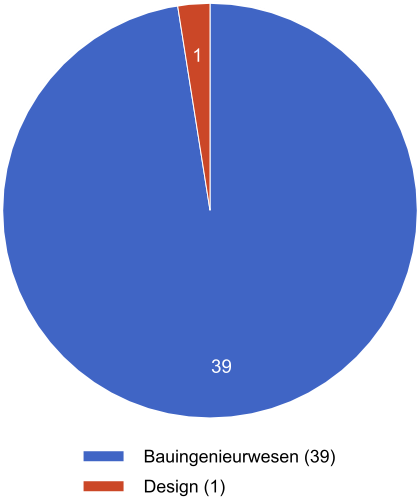
\includegraphics[width=0.4\textwidth]{torte_bauingenieur}
    \caption{Welcher Studiengang ist ähnlich zu Architektur? (Aufgabe 1)}
    \bildquelle{Eigene Darstellung}
    \label{fig:prototyp-umfrage-bauingenieur}
\end{figure}

In Aufgabe 1 sollten die Studienteilnehmer herausfinden, welcher Studiengang dem Studiengang "Architektur" ähnlich ist. Als Hilfsmittel stand ihnen der Live-Prototyp zur Verfügung. Wie in den vorherigen Kapiteln erläutert, werden ähnliche Studiengänge durch den MDS-Algorithmus nahe beieinander platziert. Die Lösung war daher der Studiengang \glqq Bauingenieurwesen\grqq{} (siehe \autoref{fig:prototyp-umfrage-bauingenieur-erklaerung}). 39 von 40 Studierenden (97,5 \%) lösten diese Aufgabe richtig. Die einzige falsche abgegebene Antwort entsprach dem Studiengang \glqq Design\grqq{}. \glqq Design\grqq{} ist im Prototyp eine Inhaltskategorie und kein Studiengang, ist aber tatsächlich dem Studiengang \glqq Architektur\grqq{} benachbart. Die hohe Übereinstimmung mit der Lösung weist auf die Intuitivität des Konzepts hin und stärkt damit die Basis für die weitere Entwicklung.

\begin{figure}[H]
    \centering
    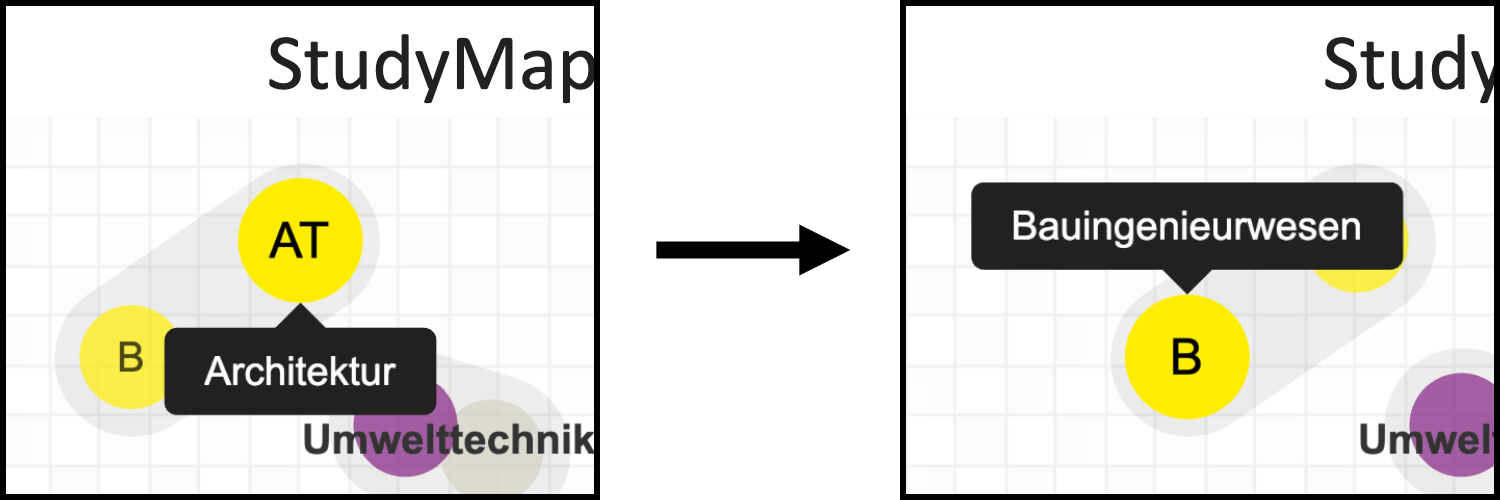
\includegraphics[width=0.65\textwidth]{prototyp_at_b}
    \caption{Prototyp: Architektur -> Bauingenieurwesen (Aufgabe 1)}
    \bildquelle{Eigene Darstellung}
    \label{fig:prototyp-umfrage-bauingenieur-erklaerung}
\end{figure}

%% Aufgabe 2

\begin{figure}[H]
    \centering
    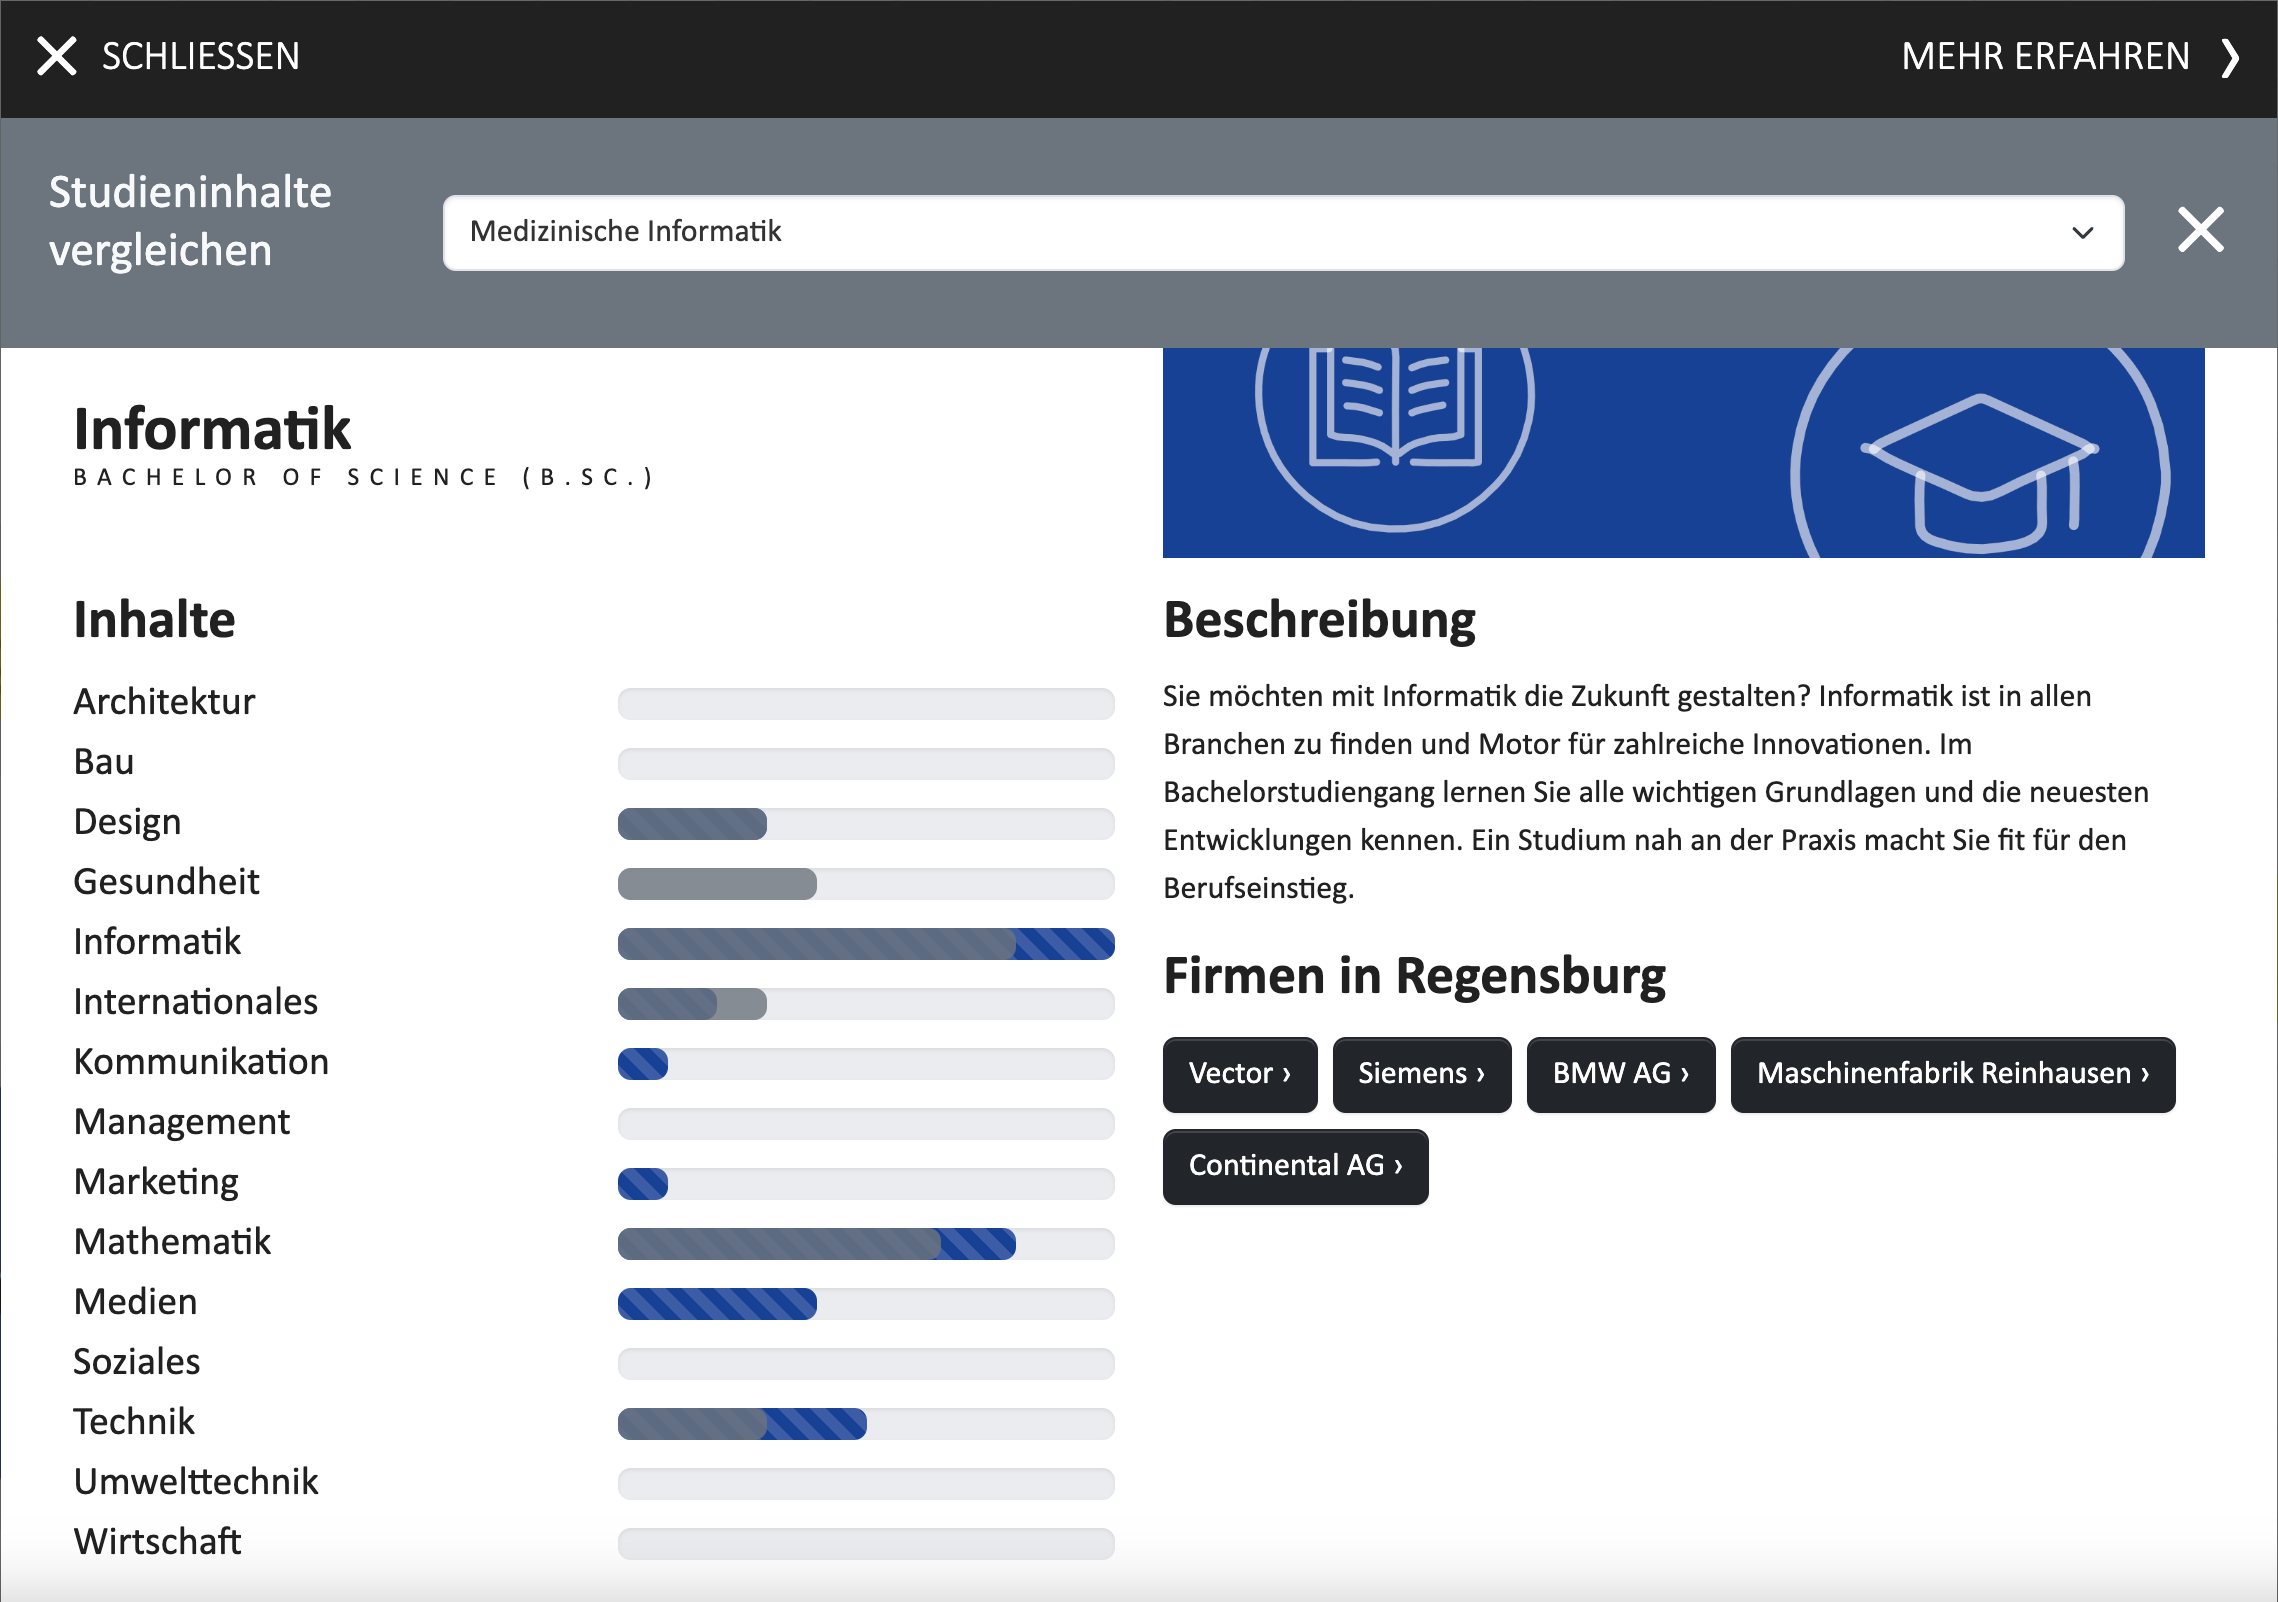
\includegraphics[width=\textwidth]{prototyp_comparison_i_im}
    \caption{Prototyp: Vergleichsfeature}
    \bildquelle{Eigene Darstellung}
    \label{fig:prototyp-comparison}
\end{figure}

In der zweiten Aufgabe sollten die Studieninteressierten herausfinden, inwiefern sich die allgemeine Informatik vom Studiengang Medizinische Informatik unterscheidet. Testweise wurde ein Feature entwickelt und zum Prototyp hinzugefügt, das es ermöglicht, Studiengänge zu vergleichen, ohne das Popup mit den Studiengangdetails schließen und erneut öffnen zu müssen.

\autoref{fig:prototyp-comparison} zeigt den Vergleich der Studiengänge Informatik und Medizinische Informatik. Die farbigen Inhaltsbalken zeigen immer die Inhalte des ursprünglich ausgewählten Studiengangs an. Wenn ein Studiengang zum Vergleich hinzugefügt wird, werden dessen Inhalte mit grauen Balken über die anderen Inhalten gelegt. Es ist wichtig, dass die Inhalte klar und verständlich dargestellt werden, ohne dabei subjektive Bewertungen einzubeziehen. Der Vergleich kann über das X-Symbol im grauen Balken gelöscht und eingeklappt werden.

\begin{figure}[H]
    \centering
    
\includegraphics[width=0.3\textwidth]{prototyp_open_comparison}
    \caption{Prototyp: Vergleichsfeature öffnen}
    \bildquelle{Eigene Darstellung}
    \label{fig:prototyp-comparison-open}
\end{figure}

Die Schülerinnen und Schüler können also mit dieser Funktion die Aufgabe bearbeiten. Wie in \autoref{fig:prototyp-comparison-open} gezeigt, kann das Feature über den mit einem Tooltip beschrifteten Knopf im Header des Popups ausgeklappt werden. Um zur Lösung zu gelangen, gibt es zwei Wege:

\begin{enumerate}
    \item Informatik-Bubble anklicken und mit Medizinische Informatik vergleichen
    \item \glqq Medizinische Informatik\grqq{}-Bubble anklicken und mit Informatik vergleichen
\end{enumerate}

Beides ergibt dasselbe Inhaltsdiagramm, aus dem sich die Unterschiede in den Studiengängen ablesen lassen.

Die Auswertung der Antworten auf Aufgabe 2 zeigt, dass die Mehrheit der Probanden das System und das Konzept hinter StudyMap verstanden hat. In \autoref{fig:prototyp-comparison-wordcloud} sind einige der genannten Schlagwörter in Form einer \textit{Wordcloud} dargestellt.

Eine Wordcloud ist eine grafische Darstellung von Textdaten. Dabei werden häufig vorkommende Wörter größer und prominenter dargestellt als seltener vorkommende Wörter. Sie bietet eine schnelle visuelle Zusammenfassung der wichtigsten Begriffe in einem Text oder einer Gruppe von Texten. Außerdem dient sie dazu, einen Überblick über die Antworten zu geben, ohne alle ausformulierten Antworten zu enthalten.

Die Begriffe \textit{Gesundheit}, \textit{Informatik}, \textit{Mathematik}, \textit{Internationales} und \textit{Medien} sind sehr prominent (siehe \autoref{fig:prototyp-comparison-wordcloud}). Bei diesen Begriffen handelt es sich um inhaltliche Kategorien, die im Prototyp verwendet werden und sich in den beiden Studiengängen unterscheiden. Daher kann die anfänglich genannte These, dass das Konzept verstanden wurde, bestätigt werden. Die Antworten der Teilnehmenden sind im Anhang ausformuliert vorzufinden.

\begin{figure}[H]
    \centering
    
\includegraphics[width=0.6\textwidth]{aufgabe2-wordcloud}
    \caption{Wordcloud der Antworten (Aufgabe 2)}
    \bildquelle{Eigene Darstellung}
    \label{fig:prototyp-comparison-wordcloud}
\end{figure}

% Später
% Schwierigkeit
Anschließend an die beiden Aufgaben wurden die Teilnehmer nach ihrer Schwierigkeitsbeurteilung befragt. Die Schüler und Schülerinnen bewerteten jeweils die Aufgaben von 1 bis 5 (1: sehr schwer, 5: sehr leicht). Anhand der folgenden \autoref{fig:prototyp-umfrage-aufgabe-1-schwierigkeit} ist erkennbar, dass die meisten Teilnehmer Aufgabe 1 als einfach empfanden.

\begin{figure}[H]
    \centering
    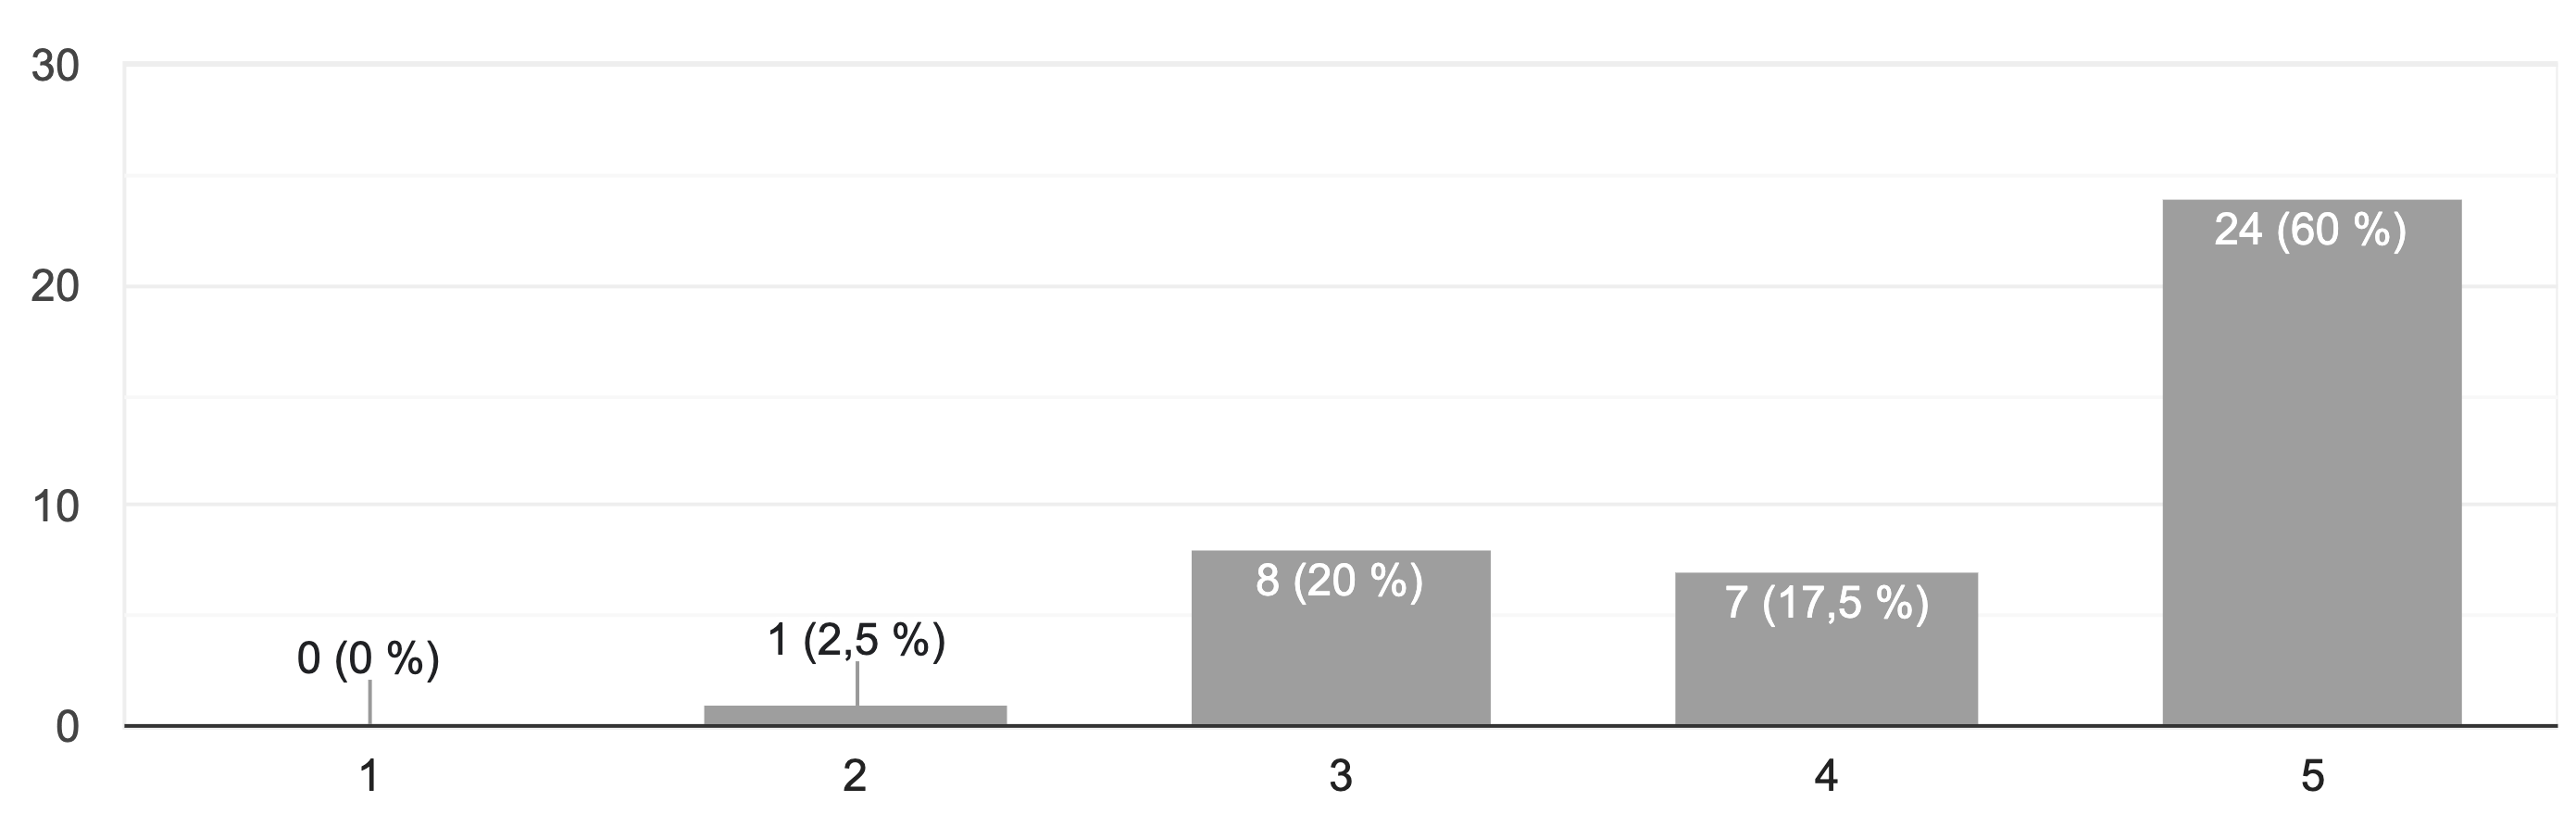
\includegraphics[width=\textwidth]{aufgabe_schwierigkeit_1}
    \caption{Wie schwer fandest du Aufgabe 1? (Auswertung Aufgabe 1)}
    \bildquelle{Google Forms}
    \label{fig:prototyp-umfrage-aufgabe-1-schwierigkeit}
\end{figure}

77,5 \% (31/40) der Befragten gaben an, dass die Aufgabe leicht zu bewältigen war (Schwierigkeitsstufe 4 oder 5). Aufgabe 2 wurde erneut als deutlich schwieriger bewertet. Obwohl 70 \% angaben, dass die Aufgabe leicht zu bewältigen war, lag das Gewicht deutlich mehr auf Schwierigkeit 4 als auf Schwierigkeit 5 (siehe \autoref{fig:prototyp-umfrage-aufgabe-2-schwierigkeit}). Ferner ist der Anstieg bei der Schwierigkeitsstufe 2 (schwer) mit 15 \% signifikant. Bei dieser Einstufung hatte die vorherige Aufgabe im Vergleich nur einen Anteil von 2,5 \% mit einer Stimme. Im Verlauf wird diese Erkenntnis durch eine \autoref{table:prototyp-umfrage-aufgaben-schwierigkeit} mit den stochastischen Werten belegt.

\begin{figure}[H]
    \centering
    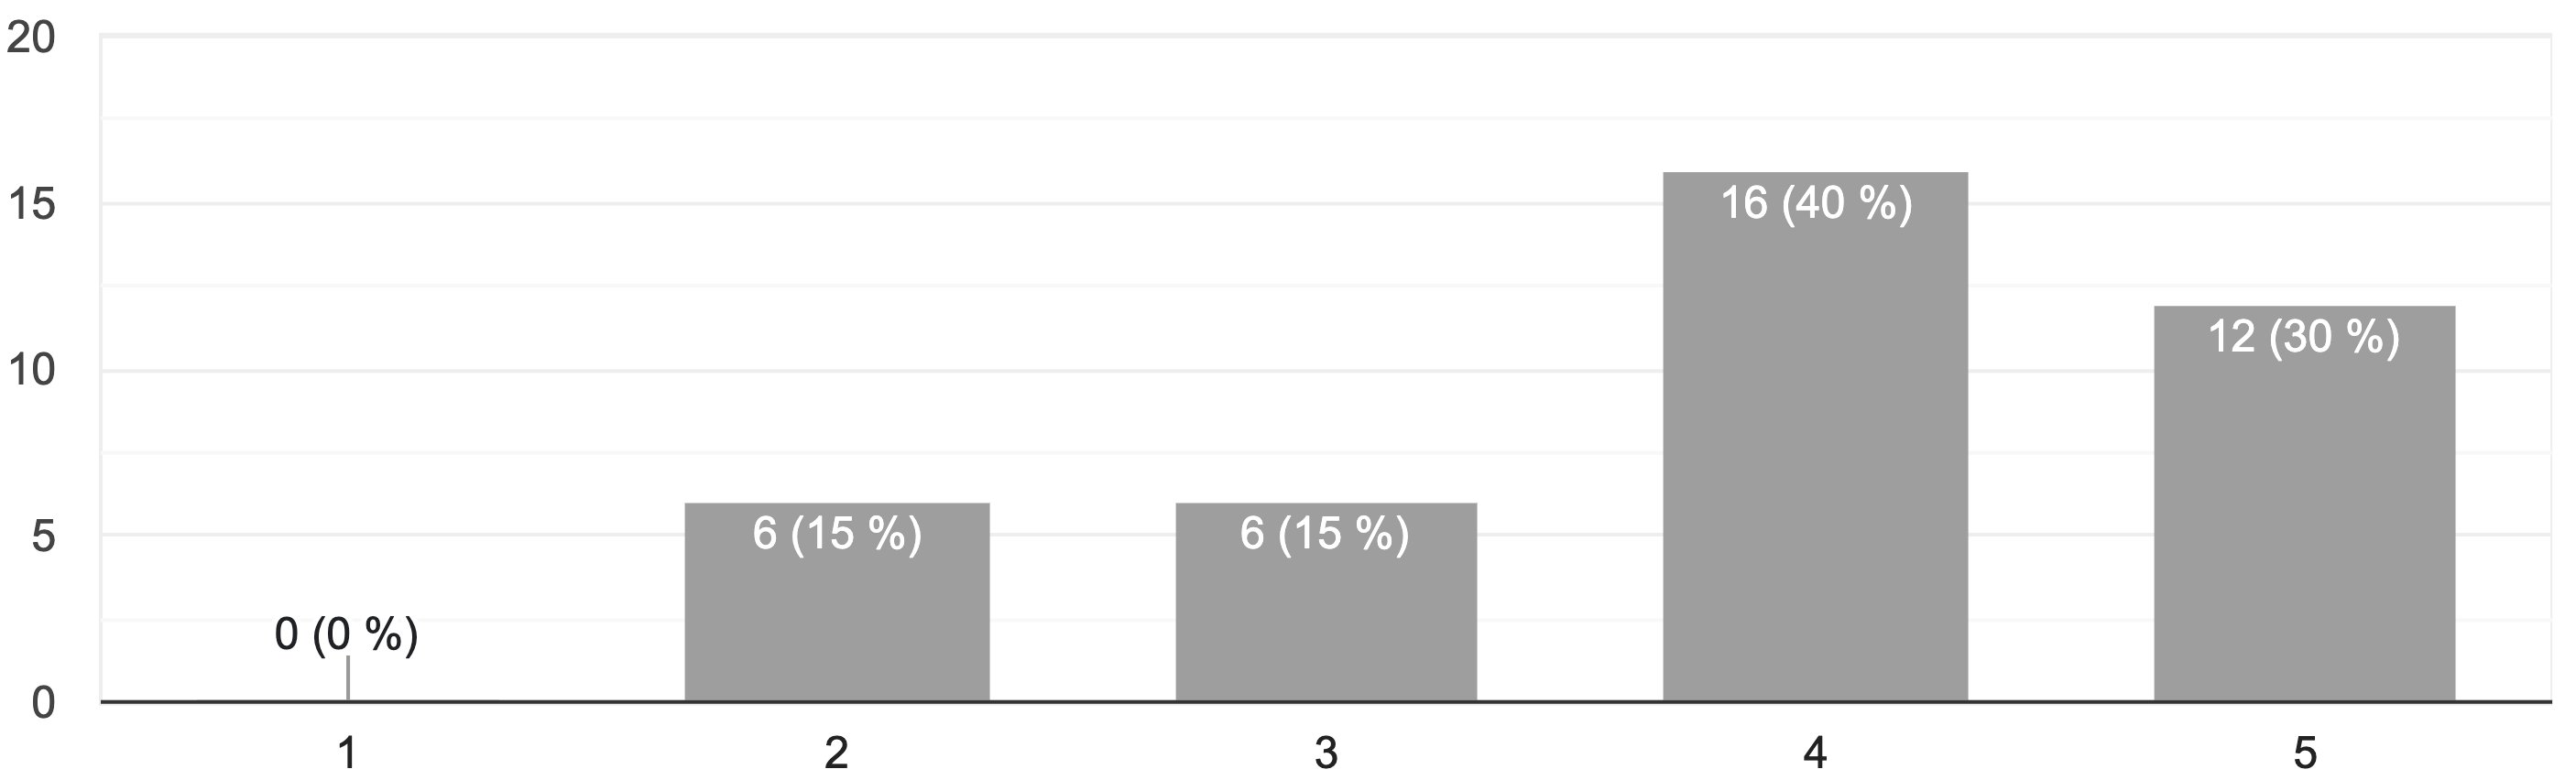
\includegraphics[width=\textwidth]{aufgabe_schwierigkeit_2}
    \caption{Wie schwer fandest du Aufgabe 2? (Auswertung Aufgabe 2)}
    \bildquelle{Google Forms}
    \label{fig:prototyp-umfrage-aufgabe-2-schwierigkeit}
\end{figure}

Zusammenfassend zeigt die stochastische Analyse in \autoref{table:prototyp-umfrage-aufgaben-schwierigkeit} die bereits aus den Diagrammen ersichtlichen Tendenzen. Sowohl der Durchschnitt als auch der Median sind bei Aufgabe 2 niedriger, was darauf hindeutet, dass diese als schwieriger empfunden wurde. Minimum und Maximum sind in beiden Aufgaben gleich. Das bedeutet, dass es bei beiden Aufgaben Befragte gab, die die Aufgaben als sehr leicht und als eher schwer empfanden. Keiner fand die Aufgaben jedoch unlösbar. Die Standardabweichung ist bei Aufgabe 2 höher als bei Aufgabe 1. Dies könnte bedeuten, dass Aufgabe 1 so einfach war, dass es für viele selbstverständlich war, die richtige Lösung zu finden und deshalb der Großteil sehr einfach ankreuzen konnte. Bei Aufgabe 2 lag der Mittelwert eher in der Mitte der Skala, weshalb die Streuung höher ist und somit die Meinungen über die Schwierigkeit stärker differierten. 

\begin{table}[H]
    \renewcommand*{\arraystretch}{1.6}
    \centering
    \begin{tabular}{|l|l|l|l|l|l|} 
    \hline
    \diagbox{\textbf{Fragen}}{\textbf{Ergebnisse}} & \textbf{Durchschnitt} & \textbf{SD} & \textbf{Median} & \textbf{Min.} & \textbf{Max.}  \\ 
    \hline
    \textbf{Wie schwer fandest du Aufgabe 1?} & 4.350 & 0.882 & 5.000 & 2 & 5 \\
    \hline
    \textbf{Wie schwer fandest du Aufgabe 2?} & 3.850 & 1.014 & 4.000 & 2 & 5 \\ 
    \hline
    \end{tabular}

    \caption{Auswertung der Fragen zu den Aufgaben}
    \label{table:prototyp-umfrage-aufgaben-schwierigkeit}
\end{table}

\paragraph{Umfrage Teil 3: Aufgaben}

Der dritte Teil der Studie beinhaltet drei Fragen, die von den Schülerinnen und Schülern in Freitextfeldern beantwortet werden konnten.  Aus diesem Grund werden auch diese Felder mithilfe von Wordclouds ausgewertet. So kann man schnell einen Überblick über die wichtigsten Punkte der Antworten erhalten.

% Was findest du am Konzept gut?

\begin{figure}[H]
    \centering
    
\includegraphics[width=0.6\textwidth]{aufgabe3.1-wordcloud}
    \caption{Wordcloud zu \glqq Was findest du an dem Konzept gut?\grqq{} (Umfrage Teil 3)}
    \bildquelle{Eigene Darstellung}
    \label{fig:prototyp-umfrage-aufgaben-3-1-wordcloud}
\end{figure}

\autoref{fig:prototyp-umfrage-aufgaben-3-1-wordcloud} zeigt die Wordcloud für die erste Frage des letzten Umfrageteils \glqq Was findest du an dem Konzept gut?\grqq{}. Wie bei der vorherigen Wortwolke sind häufig verwendete Begriffe prominenter (größer), während kleinere Begriffe nur selten verwendet wurden. Wie zuvor sind auch hier die vollständigen Antworten im Anhang zu finden. Ignoriert man die Begriffe \textit{Studiengang} und \textit{Studiengänge}, sind die Begriffe \textit{vergleichen} und \textit{Vergleich} mit insgesamt 20 Vorkommnissen sehr präsent. Es lässt sich schlussfolgern, dass die Implementierung der Vergleichsfunktion in den Prototypen erfolgreich ist und weiterverfolgt und optimiert werden sollte.

Weitere Schlagwörter, die ins Auge fallen, sind \textit{schnell}, \textit{übersichtlich}, \textit{Überblick}, \textit{direkt}, \textit{leicht}, \textit{praktisch} und \textit{ähnliche}. Diese Begriffe beziehen sich möglicherweise auf das allgemeine Konzept des Studiengangsfinders und unterstützen erneut die Basis des Konzepts, dass eine solche Art von Software bei der Studiengangsfindung für Studieninteressierte sehr nützlich sein kann.

% Was findest du am Konzept schlecht?

\begin{figure}[H]
    \centering
    
\includegraphics[width=0.6\textwidth]{aufgabe3.2-wordcloud}
    \caption{Wordcloud zu \glqq Was findest du an dem Konzept schlecht?\grqq{} (Umfrage Teil 3)}
    \bildquelle{Eigene Darstellung}
    \label{fig:prototyp-umfrage-aufgaben-3-2-wordcloud}
\end{figure}

Die zweite Frage lautete: \glqq Was findest du am Konzept schlecht?\grqq{} Für diese Frage wurde ebenfalls eine Wordcloud erstellt (siehe \ref{fig:prototyp-umfrage-aufgaben-3-2-wordcloud}). Um alle Punkte vollständig zu erfassen, wurde jedoch hauptsächlich mit den Original-Antworten gearbeitet. Der größte Begriff in Bezug auf die Zufriedenheit war \textit{nichts}, was bedeutet, dass der Großteil mit dem Prototyp bereits zufrieden war. Bei genauerer Betrachtung lassen sich jedoch einige Kritikpunkte feststellen:

\begin{itemize}
    \item Übersichtlichkeit bei vielen Bubbles
    \item Platzierung von Bubbles wirkt willkürlich
    \item Beim Vergleich ist nicht klar erkennbar, welche Farbe dem ursprünglich ausgewählten Studiengang und welche dem Vergleichsstudiengang zugeordnet ist
    \item In der Funktion \glqq Studiengang vergleichen\grqq{} sollten die Studiengänge entweder alphabetisch sortiert oder durch eine Suchfunktion filterbar sein.
    \item Legende für direkten Vergleich einfügen
    \item Die Vergleichsoption sollte auffälliger gestaltet werden
    \item Was passiert, wenn ein Studiengang inhaltlich in zwei übergeordnete Gruppen fällt?
    \item Erforderliche Soft Skill mit angeben
    \item Button \glqq Mehr erfahren\grqq{} geht in der Übersicht unter
    \item Einstiegsgehalt in absoluten Zahlen
\end{itemize}

Zusammenfassend sollte die Platzierung der Bubbles erklärt werden. Diese erfolgt nicht willkürlich, sondern mithilfe des MDS-Algorithmus und der Inhalte des Studiengangs automatisch. Im finalen Produkt werden die Bubbles voraussichtlich durch einen besseren Datensatz auch geschickter platziert, wodurch sich dieser Kritikpunkt vermutlich erledigen sollte.

Die Farbe des Vergleichsfeatures wurde mehrmals kritisiert. Im Moment werden die Inhaltsbalken des zu vergleichenden Studiengangs mit einem neutralen Grau über die des original angeklickten Studiengangs gelegt. Eine mögliche Verbesserung wäre die Verwendung einer Farbänderung, eines zusätzlichen Hilfe-Dialogs oder einer Legende. Um eine schnellere Suche zu ermöglichen, könnten die zu vergleichenden Studiengänge vor der Auslieferung ans Frontend durch das Backend alphabetisch sortiert werden.

Ferner ist es kein Hindernis, wenn ein Studiengang inhaltlich in zwei Gruppen fällt, da immer der höchste Wert zur Gruppenzugehörigkeit gewählt wird. Wenn zwei Kategorien denselben Wert haben und gleichzeitig die höchsten Werte sind, wird die erste Kategorie verwendet. Außerdem ist es kein Problem, da die Wahrscheinlichkeit hoch ist, dass die Bubbles nahe beieinander liegen, wenn der Algorithmus berechnet wird. Selbst wenn sie sich in verschiedenen Supergruppen befinden, werden sie aufgrund ihrer Koordinaten als ähnliche Studiengänge betrachtet.

Es gestaltet sich eher schwierig, erforderliche Soft Skills für das Studium anzugeben, da es keine offizielle Dokumentation über die benötigten Soft Skills pro Studiengang gibt.

Der Button \glqq Mehr erfahren\grqq{} geht in der Übersicht unter. Dieser Punkt wurde nur von einer Person geschrieben und die Schaltfläche ist bereits sehr groß und deutlich sichtbar auf der Seite rechts oben platziert, weshalb dieser Punkt nicht weiter evaluiert wird.

Es wurde zweimal nach dem Einstiegsgehalt in konkreten Zahlen gefragt. Ein Nachteil dieser Implementierung besteht darin, dass die Werte regelmäßig überprüft und gewartet werden müssen, im Gegensatz zur aktuellen Implementierung mit den einfachen Bewertungen \glqq Überdurchschnittlich\grqq{}, \glqq Durchschnittlich\grqq{} usw. Deshalb wird dieser Punkt auch nicht weiter untersucht.

% Hast du neue Ideen für den Prototypen?
% Text: Auch hier muss mit den ganzen Antworten gearbeitet werden
\begin{figure}[H]
    \centering
    
\includegraphics[width=0.6\textwidth]{aufgabe3.3-wordcloud}
    \caption{Wordcloud zu \glqq Hast du neue Ideen für den Prototypen?\grqq{} (Umfrage Teil 3)}
    \bildquelle{Eigene Darstellung}
    \label{fig:prototyp-umfrage-aufgaben-3-3-wordcloud}
\end{figure}

Die in \autoref{fig:prototyp-umfrage-aufgaben-3-3-wordcloud} genannten Punkte ähneln sehr den Kritikpunkten, die in der vorherigen Frage \glqq Was findest du an dem Konzept schlecht?\grqq{} behandelt wurden. Im Folgenden werden die Kritikpunkte auf Basis der Wordcloud und den vollen Antworten der Teilnehmenden gruppiert und zusammengefasst dargestellt. Die Original-Antworten sind, wie bei den vorherigen Fragen auch, im Anhang aufgeführt.


\begin{itemize}
    \item Vergleichsfunktion optisch ansprechender gestalten
    \item Vergleichsfunktion über mehr als zwei Studiengänge
    \item Suchfunktion zur Vergleichsfunktion hinzufügen
    \item Persönlichkeitstest einführen (als Orientierung)
    \item Ähnliche Studiengänge anders platzieren/gestalten
    \item Absolute Werte bei Gehälter
    \item Mehr Informationen zu den einzelnen Fächern ggf. Bezug auf die Schule
    nehmen
    \item Farben ändern
\end{itemize}
%% Punkte einfügen

Die optische Gestaltung der Vergleichsfunktion wurde mehrmals erwähnt. Die Farben und die Gestaltung des Buttons zur Aktivierung der Vergleichsfunktion sowie der Inhaltsbalken sollten geändert werden. Außerdem wurde der Wunsch geäußert, dass man mehr als zwei Studiengänge gleichzeitig vergleichen kann. Es stellt sich jedoch die Frage, ob dies sinnvoll ist, da es auf mobilen Endgeräten schnell unübersichtlich werden könnte. Ein weiterer oft genannter Wunsch ist eine Suchfunktion innerhalb der Vergleichsfunktion. Dies könnte, wie bei der vorherigen Frage bereits beschrieben, entweder durch eine alphabetisch sortierte Liste oder durch ein Autocomplete-Textfeld gelöst werden. Ein Autocomplete-Textfeld schlägt Vorschläge vor, während Buchstaben eingegeben werden. Es ähnelt somit einem Suchfeld.

Außerdem wurde mehrfach ein Persönlichkeitstest gewünscht, der spezifische Fragen an den oder die Studieninteressierte stellt und daraus eine Empfehlung für das zu wählende Studium ableitet. Wie bereits in \autoref{sec:konzepte-von-studiengangsfindern} erwähnt, bringt dies jedoch auch einige Limitierungen mit sich. Eine Möglichkeit für die Zukunft wäre, eine optionale Online-Umfrage anzubieten. Diese könnte die Ergebnisse aufgrund der eingegebenen Daten in StudyMap als eine Art Heatmap darstellen und die Zugehörigkeit zu einer bestimmten Position und somit zu einer Supergruppe bzw. Studiengang markieren. Eine Heatmap ist eine grafische Darstellung von Daten, bei der Werte in einer Matrix durch Farben codiert werden. Intensivere Farben repräsentieren höhere Werte, um Muster oder Trends visuell hervorzuheben. In diesem Fall werden die Zugehörigkeiten zur Kategorie \glqq Wirtschaft\grqq{} dargestellt. 

Es wurde erwähnt, dass die Sektion \glqq Ähnliche Bachelor-Studiengänge\grqq{} nicht gut platziert ist. Dieser Eindruck könnte aufgrund der eher standardmäßigen Gestaltung (siehe \autoref{fig:mockup-bubbles-popup} ganz unten im Popup) entstehen. Eine Möglichkeit wäre, die Studiengänge mit Icons zu versehen oder sie wie bei dem Abschnitt \glqq Firmen in Regensburg\grqq{} mit schwarzen, abgerundeten Rechtecken als Schaltflächen zu präsentieren.

Absolute Werte bei den Gehältern können aus den vorher genannten Gründen nicht umgesetzt werden.

Für die Kurzübersicht wäre es vermutlich zu umfangreich, Informationen zu den einzelnen Fächern bereitzustellen. Das Popup ist bereits sehr voll - mehr Inhalt könnte die Benutzererfahrung negativ beeinflussen. Ein zusätzlicher Reiter für alle Fächer wäre vermutlich zu viel. Um die einzelnen Fächer einzusehen, muss der Interessierte lediglich auf den Button \glqq Mehr erfahren\grqq{} klicken und schließlich den Studienverlaufsplan des jeweiligen Studiengangs öffnen. Dort sind alle präzisen Informationen über den Studiengang für den Benutzer zu finden. StudyMap bietet einen Überblick und eine grobe Orientierungshilfe für das Studium. Für weitere Informationen steht Studieninteressierten die OTH-Website mit detaillierten Informationen zu allen Studiengängen zur Verfügung.

Wie bereits in \autoref{sec:visualisierung-der-studiengänge} erläutert, werden die Bubbles in den Fakultätsfarben eingefärbt. Dies ist eine Anforderung der Vizepräsidentin der OTH-Regensburg und der Fakultäten der Hochschule. Daher kann dem Wunsch nach anderen Farben nicht entsprochen werden. Andere Farben könnten zu Verwirrung führen, da nicht klar ist, warum eine bestimmte Bubble beispielsweise grün gefärbt ist. Die aktuelle Lösung definiert klar, welcher Studiengang welche Farbe erhält. So umfasst z.B. die Supergruppe Technik nicht nur die Studiengänge der Fakultät Maschinenbau, sondern auch die Studiengänge der Fakultät für Elektro- und Informationstechnik. Obwohl die Studiengänge in derselben Supergruppe sind, kann man sie durch die Farben leichter voneinander unterscheiden.

\subsection{Zusammenfassung der Studien}
Zusammenfassend wurde durch die Anwendung der Mockup-Studie ein positiv bewertetes Konzept für den Prototypen entwickelt. Durch den Prozess des User Centered Designs wurden die späteren Benutzer von Anfang an in den Entwicklungsprozess einbezogen. Dadurch wird sichergestellt, dass die Bedürfnisse der Zielgruppe im finalen Produkt möglichst umfassend erfüllt werden.

Da die Anforderungen der Zielgruppe von Anfang an klar definiert sind, kann durch den Einsatz von UCD die Entwicklungszeit deutlich verkürzt werden. Beide Studien erzielten ähnliche Ergebnisse. Der Hauptkritikpunkt an den Entwürfen bzw. dem Prototypen ist die mangelnde Übersichtlichkeit. Zusammenfassend lässt sich festhalten, dass alle Teile des Endprodukts durch Hilfedialoge erläutert werden sollten. Es muss auch geprüft werden, ob eine Legende für die Bubbles als Erklärung erforderlich ist. Der Fokus sollte also auf der Darstellung von möglichst vielen Informationen in möglichst übersichtlicher Form liegen, um den Nutzern einen Überblick und Vergleich aller Studiengänge zu ermöglichen.

Durch die erste Mockup-Studie konnten bereits einige Schwachstellen des Entwurfs behoben werden, die bei der Implementierung des Prototypen berücksichtigt wurden. Bereits in dieser Phase konnte Entwicklungszeit eingespart werden, da Änderungen mithilfe des Mockups vor der ersten Entwicklung geplant werden konnten. Das positive Feedback auf den Prototyp im Rahmen der Prototypenstudie von 37 Studieninteressierten war eine Bestätigung für den Bedarf an StudyMap als Instrument zur Studienorientierung.

Zusammenfassend ist festzuhalten, dass die Studien erfolgreich verlaufen sind. Als Ausblick in die Zukunft könnte ein Orientierungstest interessant sein. Dieser Test würde den Studierenden anhand einiger Fragen eine Position auf der StudyMap zuweisen, damit sie sich die Studiengänge in der Nähe dieser Position genauer ansehen können. Eine weitere Idee für die Zukunft ist, dass mehr als nur zwei Studiengänge inhaltlich miteinander verglichen werden können.
\newpage

% Evaluierung und Validierung
% \section{Evaluierung und Validierung}

\subsection{Beschreibung der Evaluationsmethoden und -kriterien}

\subsection{Durchführung von Tests mit potenziellen Nutzern}

\subsection{Analyse der Ergebnisse aus den Tests}

\subsection{Diskussion der Stärken und Schwächen des Systems}
% \newpage

% Finale Implementierung
\section{Implementierung und Deployment}\label{sec:implementierung-und-deployment}
\subsection{Technologieauswahl und Implementierungsdetails}
Die Auswahl der geeigneten Technologien für die Entwicklung des innovativen Studiengangsfinders wurde so getroffen, dass eine effiziente und interaktive Lösung gewährleistet ist. Besonders wichtig ist die Nutzbarkeit auf Smartphones und Desktop-Geräten, wodurch sich außerdem neue Herausforderungen hinsichtlich der Bedienung ergeben. Im Folgenden werden die Hauptkomponenten des Technologiestacks und ihre jeweiligen Funktionen erläutert.

\subsubsection{PixiJS - Interaktive Grafik}
Für die Darstellung der interaktiven Grafik wurde PixiJS gewählt. PixiJS ist ein leistungsstarkes WebGL-Rendering-Framework, das eine schnelle und reibungslose Darstellung von Grafiken ermöglicht. \parencite{pixijs_pixijs_2023} WebGL (Web Graphics Library) ist eine JavaScript-Schnittstelle zur Berechnung hochperformanter, interaktiver 2D- und 3D-Grafiken zur Anzeige im Browser. \parencite{mozilla_corporation_webgl_2023} Da nicht jeder Browser WebGL unterstützt, verwendet PixiJS als Ausweichlösung immer das klassische HTML5 Canvas ohne Hardwareunterstützung. \parencite{pixijs_pixijs_2024}

Die Entscheidung für PixiJS basiert auf seiner Effizienz bei der Verarbeitung komplexer 2D-Grafiken und seiner Fähigkeit, eine ansprechende Benutzererfahrung zu bieten. Neben PixiJS wurden verschiedene weitere Bibliotheken betrachtet:
\begin{itemize}
    \item three.js: WebGL 3D-Framework
    \item D3.js: 2D-Datenvisualisierungsbibliothek
    \item Chart.js: HTML5-Bibliothek für Diagramme
    \item Paper.js: HTML5-Bibliothek für Animationen und interaktive Grafiken
    \item Fabric.js: 2D-Canvas Bibliothek
\end{itemize}

% TODO: Quellen für die "Forenthreads" gegen die Frameworks etc verlinken

Der Studiengangsfinder erfordert eine 2D-Grafikdarstellung, weshalb
\textit{three.js}, das auf 3D-Visualisierungen spezialisiert ist, nicht als
geeignete Grundlage gewählt wurde. \parencite{threejs_threejs_2023}

Die Entscheidung gegen die Verwendung von \textit{D3.js} wurde aufgrund
von Bedenken bezüglich der Dokumentation und der Wahrnehmung in der 
Entwicklergemeinschaft getroffen. Die unvollständige Dokumentation und
bestehende Forenthreads, die die Relevanz von D3.js in Frage stellen, könnten zu
potenziellen Schwierigkeiten bei der Entwicklung und zukünftigen Wartungen
führen. \parencite{bostock_d3js_2023}

% d3js-trend, d3js-trend-2

Aufgrund der festgestellten Einschränkungen in der Flexibilität von \textit{Chart.js} wurde gegen die Verwendung der Bibliothek entschieden. Auch wenn Chart.js die Erstellung einer Vielzahl von Diagrammen ermöglicht, hat sich gezeigt, dass die Anpassbarkeit begrenzt ist. \parencite{etimberg_chartjs_2023}

Basierend auf der wahrgenommenen Inaktivität des Projekts und den festgestellten 
Einschränkungen in Bezug auf Event-Handler wurde entschieden, \textit{Paper.js}
nicht zu verwenden. \parencite{lehni_paperjs_2023} Die begrenzten Event-Handler schränken
die Interaktionsmöglichkeiten ein, was im Kontext des Studiengangsfinders, der
eine umfassende Benutzerinteraktion für Smartphone und Desktop-Gerät erfordert,
als unzureichend erachtet wurde. \parencite{etimberg_paperjs_2023}

Obwohl \textit{Fabric.js} als vielversprechende Alternative erschien, wurde PixiJS aufgrund mehrerer Faktoren bevorzugt \parencite{zaytsev_fabricjs_2023}. Der Auftritt der PixiJS-Website vermittelte den Eindruck einer etablierten und professionellen Plattform, was das Vertrauen in die Stabilität und Wartbarkeit des Frameworks stärkte. Ein weiterer bedeutender Punkt ist die Anzahl der GitHub-Sterne in Relation zu der Anzahl an \textit{offenen Issues}, die PixiJS aufweist. Eine höhere Anzahl an GitHub-Sternen mit gleichzeitig weniger offenen Issues, deutet oft auf eine größere und aktivere Entwicklergemeinschaft hin, was wiederum auf kontinuierliche Weiterentwicklung und Wartung schließen lässt. \parencite{batista_github_2023}

Mit Hilfe der in den folgenden Kapiteln vorgestellten Webschnittstelle werden Daten für die Visualisierung der Studiengänge vom PixiJS-Projekt abgerufen. Anschließend werden die Studiengänge auf einer Canvas-Fläche in Form von Bubbles platziert, die sich hinsichtlich ihrer Nähe durch die Ergebnisse des MDS-Algorithmus unterscheiden:

\begin{lstlisting}[style=Python]
const x = ((renderedSize.width * 0.75) * data[i][4][0]) + renderedSize.width * 0.125;
const y = ((renderedSize.height * 0.8) * (1 - data[i][4][1])) + renderedSize.height * 0.10;
\end{lstlisting}

Die vorliegende Implementierung berechnet die x- und y-Koordinaten für die Platzierung der Studiengangs-Bubbles innerhalb des Canvas. In diesem Fall enthält die Variable \code{renderedSize} die Breite des Canvas in Relation zur physischen Pixeldichte. Die Variablen \code{data[i][4][0]} und \code{data[i][4][1]} enthalten die vom Algorithmus berechneten auf eins normierte Koordinaten. Durch Multiplikation der Breite und Höhe der gezeichneten Fläche mit einem Pufferwert (z.B. 0.75) werden die Bubbles zentriert und gleichzeitig dabei nicht bis zum Rand gezeichnet. Andernfalls könnte es vorkommen, dass die Bubbles, deren x- oder y-Koordinaten mit 0 oder 1 berechnet wurden, genau am Rand stehen und somit aufgrund der Zentrierung des Ankerpunktes des Kreises nur zur Hälfte sichtbar sind.

\begin{figure}[H]
    \centering
    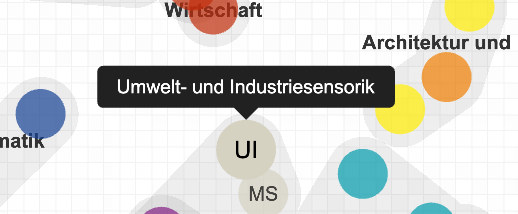
\includegraphics[width=0.6\textwidth]{pixijs-tooltip-1}
    \caption{StudyMap: Tooltip über Bubble}
    \bildquelle{Eigene Darstellung}
    \label{fig:pixijs-tooltip-1}
\end{figure}

Die Implementierung beinhaltet außerdem die Funktionalität, dass ein Tooltip erscheint, wenn man mit der Maus über eine Bubble fährt (siehe \autoref{fig:pixijs-tooltip-1}). In der Entwicklung treten dabei jedoch zwei große Herausforderungen auf: Wie funktioniert dieses Feature auf einem Smartphone ohne Maus? Was passiert, wenn das Tooltip außerhalb des Bildschirms gezeichnet wird?

% TODO: Bei Bedienung muss noch die Hitarea beim Hovern dazukommen.
\paragraph*{Herausforderung 1: Bedienung}
PixiJS verfügt über ein ereignisbasiertes System zur Verfolgung von Interaktionen mit der Zeichenfläche. Es gibt verschiedene Eventtypen, wie zum Beispiel \code{.click()}. Dieses Event wird ausgelöst, wenn auf das Objekt geklickt wird, auf dem der sogenannte Eventlistener aktiviert wurde. \parencite{pixijs_interaction_2024}

Für das Tracking, ob der Benutzer mit der Maus über der Bubble ist, wird der Eventtyp \code{.onmouseover()} verwendet. Die Studiengänge werden, wie im Konzept vorgestellt, in Supergruppen eingeteilt. Alle Studiengänge, die zur gleichen Supergruppe gehören, werden durch ein Label mit dem Namen der Supergruppe und einen leichten Hintergrundnebel gekennzeichnet, um ihre Zugehörigkeit zu zeigen. Ohne Interaktion mit dem Canvas werden die Studiengänge nicht beschriftet, sondern nur als farbige Kreise dargestellt. (siehe \autoref{fig:pixijs-canvas-2}).

\begin{figure}[H]
    \centering
    
\includegraphics[width=0.3\textwidth]{pixijs-canvas-2}
    \caption{StudyMap: Supergruppe mit Label}
    \bildquelle{Eigene Darstellung}
    \label{fig:pixijs-canvas-2}
\end{figure}

Beim Berechnen des Nebels der Supergruppen werden gleichzeitig die Minima und Maxima der x- und y-Koordinaten berechnet. Das Ergebnis ist ein unsichtbares Rechteck, das alle Studiengänge in dieser Inhaltskategorie umfasst; dieses Rechteck hat die Funktion einer Hitarea. Auf dieser Hitarea wird ein \code{.onmouseover()}-Eventlistener platziert, der ausgelöst wird, sobald der Benutzer mit der Maus in die Nähe eines Studiengangs dieser Kategorie kommt.

Sobald dieser Fall eintritt, wird das Label der Supergruppe deaktiviert und alle Studiengangs-Bubbles erhalten als Label das Kürzel des jeweiligen Studiengangs (siehe \autoref{fig:pixijs-canvas-3}).

\begin{figure}[H]
    \centering
    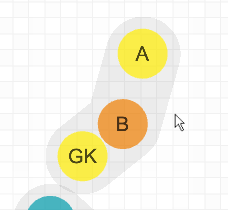
\includegraphics[width=0.3\textwidth]{pixijs-canvas-3}
    \caption{StudyMap: Supergruppe ohne Label - Hitarea}
    \bildquelle{Eigene Darstellung}
    \label{fig:pixijs-canvas-3}
\end{figure}

Schließlich besitzt jede Bubble einen zusätzlichen \code{.onmouseover()}-Eventlistener. Wenn dieses Event ausgelöst wird, wird die Bubble vergrößert und immer gegenüber eventuell überschneidenden Bubbles in den Vordergrund gestellt. Die Labels der anderen Studiengänge in allen anderen Supergruppen werden deaktiviert, um den Fokus auf diese Inhaltskategorie und explizit diesen Studiengang zu legen. Daraufhin erscheint darüber das Tooltip, das in \autoref{fig:pixijs-tooltip-1} zu sehen ist. Ein Klick auf die fokussierte Bubble oder den dargestellten Tooltip öffnet das Popup mit den Details zum Studiengang.

Da ein Smartphone in der Regel keine Maus angeschlossen hat, wird anstelle des für Desktop-Benutzer verwendete \code{.onmouseover()}-Event das \code{.ontap()}-Event verwendet. Dieses Ereignis wird ausgelöst, wenn der Benutzer auf die Bubble des Studiengangs tippt. Die Hitarea des Supergruppen-Nebels wird dabei auf Smartphones ignoriert.

Auch hier muss erneut differenziert werden. Wenn ein Desktop-Nutzer auf eine Bubble klickt, öffnet sich gemäß dem Konzept der Dialog mit den Studiengangsdetails. Tippt ein Smartphone-Nutzer auf die Bubble, sollte sich das Popup nicht direkt öffnen. Es ist wichtig, dass der Nutzer zuvor das Tooltip gesehen hat, um zu wissen, welchen Studiengang er öffnet.

Aus diesem Grund wird beim \code{.ontap()}-Event auf eine Bubble zwischen drei Zuständen unterschieden:

\begin{enumerate}
    \item \textbf{Bisher noch keine andere Bubble angetippt:} Sollte bisher noch keine Bubble selektiert oder angetippt worden sein, wird der gleiche Hover-Effekt ausgeführt, den auch ein Desktop-Endgerät beim \code{.onmouseover()}-Event über eine Bubble auslösen würde.
    \item \textbf{Es wurde bereits eine andere Bubble angeklickt:} In diesem Fall wird der Hover-Effekt für die bereits angeklickte Bubble deaktiviert und für diese Bubble aktiviert.
    \item \textbf{Diese Bubble wurde bereits angeklickt:} Daraufhin wird das Tooltip entfernt und das Popup mit den Details zum Studiengang geöffnet. Dies ist das Äquivalent zu einem Doppelklick auf die Bubble.
\end{enumerate}

Zur Implementierung dieser Funktionalität ist die Zwischenspeicherung eines Active-State erforderlich, der immer die zuletzt angeklickte Bubble enthält.

\paragraph*{Herausforderung 2: Was passiert, wenn das Tooltip außerhalb des Bildschirms gezeichnet wird?}
Die Zeichenoberfläche von PixiJS enthält keine vorgefertigten Anzeigeelemente oder Komponenten zur Erstellung einer Benutzeroberfläche. Das bedeutet, dass Elemente wie z.B. das Tooltip in Abbildung X selbst mit Hilfe von Polygonen gezeichnet werden müssen.

Das gezeigte Tooltip besteht aus einem abgerundeten Rechteck, das den Text darüber enthält, und einem Dreieck, das anzeigt, für welche Bubble das Tooltip geöffnet wurde. Das Rechteck und das dazugehörige Dreieck werden in Schwarz aneinander gesetzt, so dass das kleine Fenster wie eine Sprechblase aussieht.

Die Standardrichtung zum Öffnen des Tooltips wurde bei der Entwicklung der Klasse Tooltip nach oben festgelegt. Der folgende Codeausschnitt zeigt, wie die Richtung festgelegt wird:

\begin{lstlisting}[style=Python]
this.direction = 'top';
if (this.rootObjectYPosition - this.distance - this.container.height < 0) {
    // if object is too high to display the tooltip, it will be drawn to the bottom
    this.direction = 'bottom';
} else if (this.rootObjectXPosition - this.container.width / 2 < 0) {
    // if object overlaps left world border, it will be drawn to the right        
    this.direction = 'right';
} else if (this.rootObjectXPosition + this.container.width / 2 > this.worldWidth) {
    // if object overlaps right world border, it will be drawn to the left
    this.direction = 'left';
}
\end{lstlisting}

Die Variablen \code{this.rootObjectXPosition} und \code{this.rootObjectYPosition} enthalten die x- und y-Koordinaten des Elements, an dem der Tooltip erscheinen soll. In diesem Fall sind dies die Koordinaten der jeweiligen Bubble. Die Variable \code{this.distance} enthält den vordefinierten Abstand, um den der Tooltip vom Element entfernt sein soll. Im vorliegendem Fall handelt es sich mindestens um den Radius des Studiengangskreises. Die Größe des Tooltips wird wiederum in den Variablen \code{this.container.height} und \code{this.container.width} gespeichert.

Die Richtung des Tooltip-Fensters wird nach dem Ausschlussverfahren festgelegt. Wenn das Tooltip mit der Standardrichtung \code{'top'} (nach oben) aus der Zeichenfläche hinausragt, wird die Richtung nach unten (\code{'bottom'}) geändert. Anschließend wird überprüft, ob das Element die linke Fenstergrenze überschreitet. Falls dies der Fall ist, wird die Richtung auf \code{'rechts'} gesetzt. Analog dazu wird geprüft, ob das Objekt die rechte Grenze überschreitet. In diesem Fall wird die Richtung auf \code{'links'} gesetzt.

Sobald die Ausrichtung des Tooltips festgelegt wurde, müssen die Elemente einzeln verschoben und gedreht werden. Führt die vorangegangene if-Bedingung dazu, dass die Richtungsvariable \code{direction} auf \code{'left'} gesetzt wird, muss das Tooltip wie in der folgenden \autoref{fig:pixijs-tooltip-2} dargestellt links neben der Bubble erscheinen.

\begin{figure}[H]
    \centering
    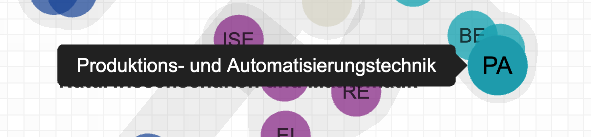
\includegraphics[width=0.6\textwidth]{pixijs-tooltip-2}
    \caption{StudyMap: Tooltip links neben Bubble}
    \bildquelle{Eigene Darstellung}
    \label{fig:pixijs-tooltip-2}
\end{figure}

Der unten dargestellte Codeauszug zeigt die Platzierung des Tooltip-Containers auf der linken Seite. Zunächst wird mit der Zeile \code{triangle.rotation = -Math.PI / 2} die Rotation des Dreiecks geändert, sodass es sich um 90 Grad nach links dreht. Anschließend werden die x- und y-Koordinaten des Dreiecks so angepasst, dass es an der rechten Seite des abgerundeten Rechtecks anliegt. Schließlich wird der gesamte Container mithilfe der Zeilen sechs und sieben linksbündig und gleichzeitig vertikal zentriert neben der Bubble platziert. Sowohl das Dreieck als auch das abgerundete Rechteck und der Text sind im Container enthalten. % TODO: Quelle Pixi Container oben erklären

\noindent
Platzierung des Tooltips auf der linken Seite:
\begin{lstlisting}[style=Python]
if (this.direction == 'left') {
    triangle.rotation = -Math.PI / 2;
    triangle.y = this.container.height / 2 - triangleHeight / 2;
    triangle.x = this.container.width;

    this.container.x = -this.container.width - this.distance;
    this.container.y = -background.height / 2;
}
\end{lstlisting}

Dieser Ansatz funktioniert jedoch nur bis zu einem gewissen Grad. Wenn das Tooltip breiter als die x-Achse des Endgeräts ist, wird es immer über die Ränder des Canvas hinausragen, da auf keiner der beiden Seiten genügend Platz für das Tooltip zur Verfügung steht. % TODO: In Zukunftsaussichten aufnehmen

\paragraph*{Popup-Dialog mit Studiengangsdetails}
Sobald das im vorigen Abschnitt beschriebene Ereignis zum Öffnen des Popups ausgelöst wird, werden die benötigten Studiengangsdetails von der später beschriebenen Webschnittstelle abgerufen und angezeigt. Zur Darstellung der Dialog-Komponente wird eine weitere Programmibliothek verwendet: Bootstrap.

Bootstrap ist ein Open-Source-Frontend-Framework für die Entwicklung von responsiven Websites und Webanwendungen. Es enthält eine Vielzahl von vordefinierten CSS-Klassen und JavaScript-Plugins, die eine Integration von Designelementen wie Buttons, Formularen und Navigationen ermöglichen. \parencite{otto_bootstrap_2024} Mit seinem integrierten Grid-System kann Bootstrap schnell an verschiedene Bildschirmgrößen angepasst werden, was den Designprozess vereinfacht und die Browserkompatibilität verbessert. \parencite{otto_browsers_2024}

Bootstrap beinhaltet eine Modal-Komponente, die als Grundlage für das Details-Popup verwendet wird. \parencite{otto_modal_2024} Diese Basis kann dann mit Hilfe von CSS-Regeln so angepasst werden, dass der endgültige Dialog in Bezug auf das Design dem Konzept von StudyMap entspricht.

Eine Herausforderung bei diesem Modal war, dass ursprünglich geplant war, dass beim Öffnen des Popups der gesamte Bildschirminhalt etwas dunkler wird und der Inhalt des Popups den Großteil des Bildschirms einnimmt. Dadurch hätte man beispielsweise an einem größeren Endgerät ein zweispaltiges Layout anstreben können. Da es sich beim iFrame um einen geschlossenen Container handelt, ist es jedoch nicht möglich, Inhalte aus dem iFrame heraus auf der einbindenden Seite darzustellen. Die mittels iFrame eingebettete Webseite kann nur innerhalb dieses iFrames wirken. % Todo: Quelle

Wegen dieser Herausforderung wird das Popup als Vollbildanzeige entwickelt, so dass es die gesamte Breite des iFrames einnimmt und nur vertikales Scrollen erlaubt (siehe \autoref{fig:popup-1} - roter Pfeil 1).

\begin{figure}[H]
    \centering
    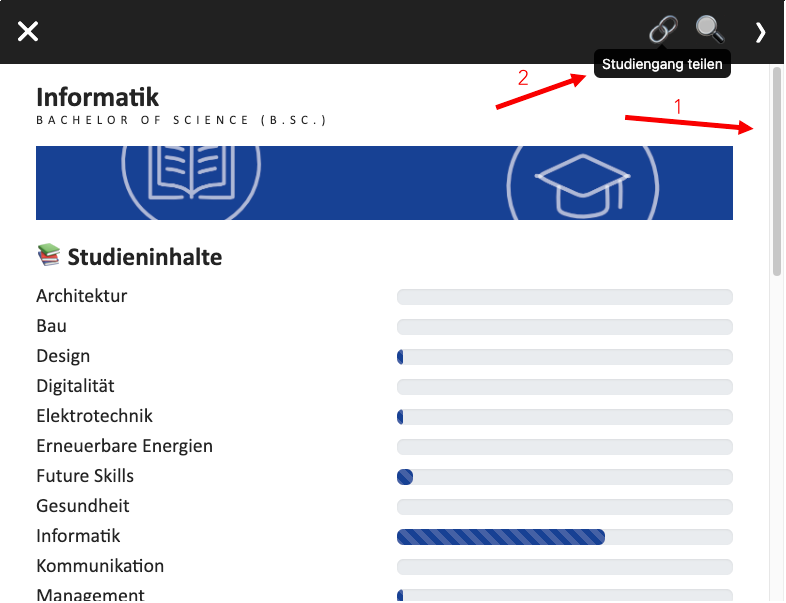
\includegraphics[width=0.6\textwidth]{popup-1}
    \caption{StudyMap: Popup-Implementierung 1}
    \bildquelle{Eigene Darstellung}
    \label{fig:popup-1}
\end{figure}

Außerdem wird in der Werkzeugleiste oben bei kleinen Anzeigegrößen auf die Beschriftung verzichtet. Anstelle von Beschriftungen werden aussagekräftige Icons verwendet und ähnlich wie bei den Studiengangsbubbles Tooltips eingesetzt, sobald die Maus darüber bewegt wird (siehe \autoref{fig:popup-1} - Pfeil 2).

In der oberen Werkzeugleiste befindet sich die Funktion zum Vergleichen der Studiengänge, wie in der UCD-Studie beschrieben. Die Aktivierung dieser Funktion erfolgt durch einen Klick auf die Lupe rechts neben dem roten Pfeil 2, wie in \autoref{fig:popup-1} dargestellt.

Das Icon links daneben enthält eine bisher noch nicht beschriebene Funktion zum Teilen des Studiengangs. Hintergrund ist, dass eine Person, die an einem Studium interessiert ist, einen passenden Studiengang finden und diesen entweder speichern oder mit engen Bekannten teilen kann. Die technische Umsetzung dieses Features wird mittels der Web Share API und der Zwischenablage des Endgerätes realisiert.

Die Web Share API ist eine browserbasierte Schnittstelle, die es Webentwicklern ermöglicht, die native Teilen-Funktionalität von Geräten zu nutzen. Sie erleichtert das direkte Teilen von Webinhalten über Messaging-Apps oder per E-Mail, ohne zusätzliche Plugins. Diese Standard-API verbessert die Benutzerfreundlichkeit und erlaubt die einfache Integration in Web-Applikationen auf verschiedenen Plattformen und OS. \parencite{mozilla_corporation_web_2023}

Wenn der Benutzer auf die Teilen-Schaltfläche tippt, wird überprüft, ob der Browser die Web Share API unterstützt. Wenn dies der Fall ist, wird ein Datenpaket mit einem eindeutigen Link zu diesem Studiengang an das Betriebssystem gesendet. Das Datenpaket enthält folgende Informationen:
\begin{itemize}
    \item \textbf{Titel:} Name des Studiengangs
    \item \textbf{Beschreibung:} \glqq An der OTH-Regensburg studieren\grqq{}
    \item \textbf{URL:} Link zum Studiengangsfinder + Queryparameter mit Kürzel des ausgewählten Studiengangs
\end{itemize}

Anschließend öffnet sich ein Fenster des Betriebssystems, um den übergebenen Link zu teilen. Das Aussehen und der Dialog können von Betriebssystem zu Betriebssystem variieren, die folgende \autoref{fig:popup-3} zeigt ein Beispiel unter macOS:

\begin{figure}[H]
    \centering
    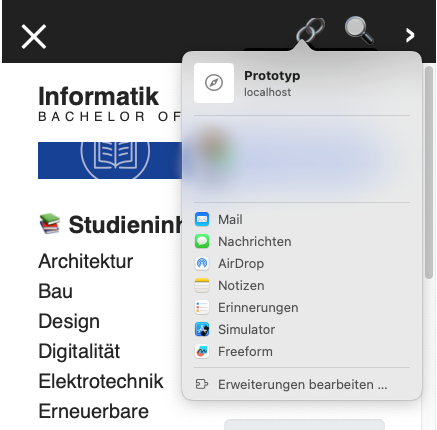
\includegraphics[width=0.5\textwidth]{popup-3}
    \caption{StudyMap: Web Share API}
    \bildquelle{Eigene Darstellung}
    \label{fig:popup-3}
\end{figure}

Falls der Browser die Web Share API nicht unterstützt, muss eine Ausweichlösung bereitgestellt werden. Um zu überprüfen, ob der Browser diese API unterstützt, gibt es mit der Methode \code{navigator.canShare()} folgende Möglichkeit zur Abfrage: \parencite{mozilla_corporation_web_2023}
\begin{lstlisting}[style=Python]
if (navigator.canShare && navigator.canShare(shareData)) {
    // Browser supports Web Share API
} else {
    // Browser does not support Web Share API
}
\end{lstlisting}

Falls die API nicht unterstützt wird, verwendet StudyMap als Ausweichlösung die Zwischenablage in Verbindung mit einer kleinen Meldung auf dem Bildschirm. Sobald der Benutzer auf den Share-Button klickt, prüft StudyMap, ob der Browser in der Lage ist, die Daten über das System zu teilen. Wenn dies nicht der Fall ist, speichert StudyMap den Link zum Teilen in der Zwischenablage des Endgeräts und benachrichtigt den Benutzer darüber mit einer Nachricht, wie in \autoref{fig:popup-4} dargestellt.

\begin{figure}[H]
    \centering
    
\includegraphics[width=0.6\textwidth]{popup-4}
    \caption{StudyMap: Studiengang teilen (ohne Web Share API)}
    \bildquelle{Eigene Darstellung}
    \label{fig:popup-4}
\end{figure}

Neben der Erzeugung des Freigabelinks muss StudyMap auch in der Lage sein, den Link zu interpretieren, damit beim Öffnen des Links das richtige Studienprogramm als Popup geöffnet wird. Da StudyMap in einem iFrame ausgeführt wird, holt sich StudyMap die URL (Uniform Resource Locator) des übergeordneten Fensters und fügt dem Link einen Queryparameter hinzu. Die URL ist eine Webadresse, die es ermöglicht, eine spezifische Ressource im Internet zu lokalisieren und darauf zuzugreifen - in diesem Fall entspricht sie dem Link der jeweiligen Website \parencite{mozilla_corporation_url_2023}.


\noindent
\textbf{Fiktives Beispiel:}\newline
URL StudyMap: \code{app.studymap.de}\newline
URL OTH-Regensburg mit StudyMap als iFrame: \code{oth-regensburg.de/studienorientierung}\newline
Freigabelink: \code{oth-regensburg.de/studienorientierung?s=<Studienkürzel>}\newline

Mithilfe des Befehls \code{window.parent.location.href} kann StudyMap die URL der Eltern-Seite abrufen. In diesem fiktiven Beispiel handelt es sich bei der URL um die URL der Website der Hochschule Regensburg, die das Canvas als iFrame eingebunden hat. An diese URL wird der Queryparameter \code{s} mit dem Wert des Studiengangskürzels gehängt. Wenn der Knopf beispielsweise im Popup für Informatik gedrückt wird, entspricht dieser Wert \code{I}, also insgesamt \code{?s=I}.

Die Übermittlung des Parameters an den iFrame stellt die eigentliche Schwierigkeit dar. Wird die URL mit dem Queryparameter geteilt und der Benutzer ruft diese Seite auf, erhält der iFrame auf der betreffenden Seite diesen Parameter nicht automatisch. Damit der Studiengangsfinder innerhalb des iFrames den Parameter erhält, muss dieser von der einbindenden Seite (in diesem Fall die Hochschulwebseite) mithilfe von JavaScript extrahiert und an die Quelladresse der StudyMap-App angehängt werden. Im Folgenden ein Beispiel für einen HTML- und JavaScript-Code zur Extrahierung des Queryparameters \code{s} und anschließender Anpassung der iFrame-Quelle mit dem übergebenen Parameter:
\begin{lstlisting}[style=Python]
<iframe src="app.html" frameborder="0" allow="web-share"
    scrolling="no" onload="resizeIframe(this)" id="studymap"></iframe>

<script>
const shareParam = new URLSearchParams(window.location.search).get('s');
if (shareParam != null) {
    document.querySelector('#studymap').setAttribute('src', `app.html?s=${shareParam}`);
}

...
</script>
\end{lstlisting}

Analog dazu ist StudyMap in der Lage, den nun übergebenen Parameter zu extrahieren und unter Verwendung des Studienkürzels beim Start der Anwendung das entsprechende Studiengangs-Popup zu öffnen. 

\begin{figure}[H]
    \centering
    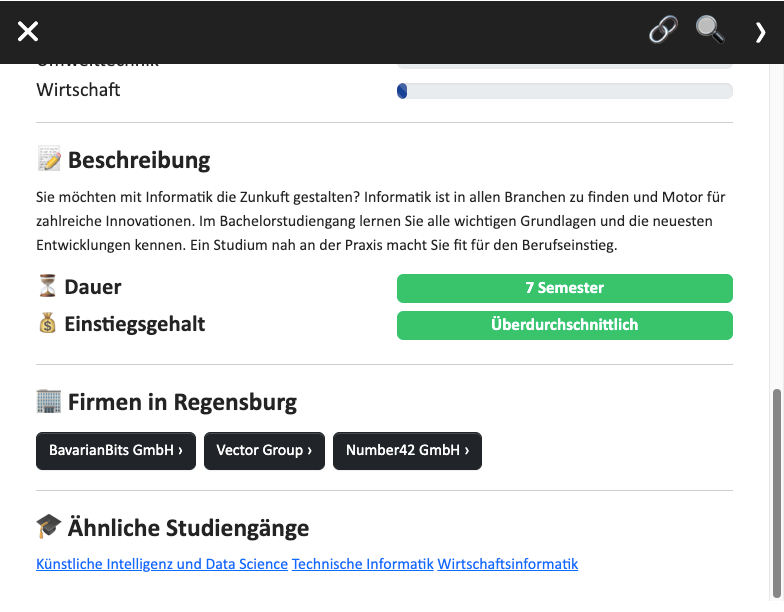
\includegraphics[width=0.7\textwidth]{popup-2}
    \caption{StudyMap: Popup-Implementierung 2}
    \bildquelle{Eigene Darstellung}
    \label{fig:popup-2}
\end{figure}

Abschließend zum Popup zeigt \autoref{fig:popup-2} den unteren Teil des Popups. Dort finden sich weitere Informationen zum Studiengang, wie z.B. Beschreibung, Dauer und Einstiegsgehalt. Darüber hinaus enthält dieser Teil des Dialogs eine Liste von Unternehmen in der Region, die Stellenangebote für den gewählten Studiengang anbieten, wie bereits im Konzept ausgeführt. Ganz unten befindet sich eine Liste mit ähnlichen Studiengängen. Diese Liste wird mithilfe des im nächsten Kapitel erläuterten Python-Skripts erzeugt.

\subsubsection{Python - Berechnung der Positionen}
Die Berechnung der Positionen für die Studiengänge basiert, wie im Abschnitt
\ref{sec:MDS} erläutert, auf dem Multidimensionalen Skalierungsalgorithmus
(MDS), der in Python implementiert ist. Der Algorithmus verarbeitet eine
strukturierte CSV-Datei, die alle relevanten Informationen zu den Studiengängen,
Feldern und Meta-Informationen (wie z.B. Fakultätszugehörigkeit) enthält. Dieser
Datensatz bildet die Grundlage für die Positionsbestimmung im zweidimensionalen
Raum.

Hierzu wird ein Python-Skript entwickelt, welches die CSV-Datei einliest und
schließlich den MDS-Algorithmus auf den Daten anwendet. Im Verlauf der
Arbeit wurde eine anfängliche Eigenimplementierung des MDS-Algorithmus in
Betracht gezogen.

\noindent
Zu diesem Zweck wurde eine Python-Klasse erstellt, die drei Methoden enthält:
\begin{enumerate}
    \item calculate\_distance\_matrix(X)
    \item read\_data\_from\_csv()
    \item mds(self)
\end{enumerate}

Die Methode \code{calculate\_distance\_matrix} berechnet die Distanzmatrix,
welche für den Ablauf des Programms essenziell ist. Der Code dazu wird an
dieser Stelle ausgespart, da er bereits in Abschnitt \ref{sec:distanzmatrix}
vollständig spezifiziert wurde. Außerdem ausgespart ist die Methode
\code{read\_data\_from\_csv()}, welche die Eingabedatei einliest, analysiert und
schließlich die zur Berechnung benötigten Zahlen-Arrays zurückgibt. Für die Berechnung der mathematischen Gleichungen wird die Programmbibliothek NumPy verwendet. \parencite{team_numpy_2023}

\noindent
\begin{minipage}{\linewidth}
Folgender Ausschnitt eines Quellcodes beinhaltet die für diese
Arbeit entwickelte Eigenimplementierung des MDS-Algorithmus, basierend auf dem im Abschnitt
\ref{sec:MDS} genau erläuterten Ablauf:
\begin{lstlisting}[style=Python]
def mds(self):
    # Reads data from CSV file and transforms it to number rows
    X = self.read_data_from_csv()

    # Calculates distance matrix
    M = self.calculate_distance_matrix(X)

    # Double centered matrix
    n = 11 # Number of subjects
    I = np.identity(n) # Identity matrix
    Jn = np.ones((n, n)) # Matrix Jn of all ones
    C = I - (1/n) * Jn # Calculate centering matrix C
    B = -0.5 * np.dot(np.dot(C, np.array(M)), C) # Calculate the double centered matrix B

    # Eigenvalues, Eigenvectors
    m = 2  # number of dimensions (2D)
    eigenvalues, eigenvectors = np.linalg.eig(B) # Perform eigenvalue decomposition

    # Sort eigenvalues and corresponding eigenvectors in descending order
    sorted_indices = np.argsort(eigenvalues)[::-1]
    eigenvalues = eigenvalues[sorted_indices]
    eigenvectors = eigenvectors[:, sorted_indices]

    # Select the top m eigenvalues and corresponding eigenvectors
    top_m_eigenvalues = eigenvalues[:m]
    top_m_eigenvectors = eigenvectors[:, :m]

    # Calculate the square root of the diagonal matrix
    sqrt_Lambda_m = np.sqrt(np.diag(top_m_eigenvalues))

    # Compute the matrix X using the formula
    X_transformed = np.dot(top_m_eigenvectors, sqrt_Lambda_m)

    return X_transformed
\end{lstlisting}
\end{minipage}

Die Entwicklung und Umsetzung dieser eigenen Lösung erwies
sich jedoch als äußerst anspruchsvoll, da sie zahlreiche subtile mathematische
Nuancen berücksichtigen müsste. Angesichts dieser Komplexität wurde die
Entscheidung getroffen, auf die bewährte und leistungsstarke
SciKit-Learn-Bibliothek zurückzugreifen. Die Verwendung dieser etablierten
Implementierung ermöglicht eine präzise und effiziente Lösung, wobei der Fokus
auf den zentralen Fragestellungen der Masterarbeit bleibt. Außerdem gewährleistet
die Einbindung von SciKit-Learn neben der Robustheit der MDS-Umsetzung, auch die
Reduktion der Entwicklungskomplexität im Hinblick auf die
Algorithmusimplementierung. \parencite{developers_scikit-learn_2023}

Das Ergebnis des Skripts sind Koordinaten für jeden Studiengang im zweidimensionalen Raum. Diese Koordinaten werden anschließend auf eins normiert und zusammen mit den vorher eingelesenen Meta-Daten zu den Studiengängen in JSON-Dateien gespeichert, die schließlich vom Backend über eine Webschnittstelle bereitgestellt werden.

Der Vorteil bei der Speicherung der berechneten Positionen in Form von
JSON-Dateien liegt darin, dass die Daten wesentlich seltener geändert werden,
als die Website aufgerufen wird. Somit wird effektiv Rechenleistung und Strom
gespart. Gleichzeitig erhöht
dieses Vorgehen die Performance der Website. Zur Festigung dieser These werden
die Google Suchtrends von 2021 zum Suchbegriff \glqq OTH Regensburg
Studiengänge\grqq{} herangezogen (siehe Anhang
\ref{appendix:google-search-trends}). Die Trends zeigen eine Jahressumme von
1194 Suchanfragen. Die Anzahl an Suchanfragen lassen sich nicht 1:1 in
Seitenaufrufe projizieren, verdeutlichen aber dennoch einen ungefähren
Richtwert. Die Datengenerierung hingegen wird nach mündlicher Zusage von
Frau Rösel (Vizepräsidentin der OTH-Regensburg) nur bei größeren Änderungen an den
Inhalten von Studiengängen, oder beim Hinzufügen bzw. Entfernen eines 
Studiengangs ausgelöst. Dies wiederum passiere meist insgesamt nur einmal pro
Jahr.

Das Python-Skript hat neben der Berechnung und Speicherung der Koordinaten der Studiengänge noch eine weitere Aufgabe. Sobald der Benutzer auf der StudyMap eine Bubble anklickt, öffnet sich ein Popup mit Details zum entsprechenden Studiengang (siehe Konzept \autoref{fig:mockup-bubbles-popup}). Wie im weiteren Verlauf der Arbeit noch erläutert wird, können diese Details über die Administrationsoberfläche bearbeitet werden. Um die Details in der Administrationsmaske bearbeiten zu können, legt das Python-Skript für jeden Studiengang eine .json-Datei mit den erforderlichen Attributen an. Gleichzeitig werden die ähnlichen Studiengänge, die durch den MDS-Algorithmus berechnet wurden, sowie die Werte der Inhaltskategorien eingefügt.

Bei der Berechnung neuer Koordinaten wird, wie im vorherigen Abschnitt erwähnt, für jeden eingelesenen Studiengang eine .json-Datei mit einem leeren Template erstellt. Wenn bereits eine Datei für den Studiengang aus einer vorherigen Datenquelle existiert, wird diese geöffnet und bearbeitet. Zur späteren Darstellung der Inhaltskategorien werden anschließend die Originalwerte aus der Datenquelle in die .json-Datei kopiert (siehe folgendes Beispiel-JSON-Objekt \code{contents}).

Um ähnliche Studiengänge zu ermitteln, wird für jeden Studiengang anhand der zuvor berechneten Koordinaten der euklidische Abstand zu allen anderen Studiengängen ermittelt. Alle Studiengänge, die innerhalb einer bestimmten Grenze liegen, werden in eine Liste aufgenommen und schließlich in die .json-Datei des jeweiligen Studiengangs geschrieben (siehe folgendes Beispiel-JSON-Objekt \code{related\_studies}).

\noindent
Beispiel: Leeres Template des Studiengangs Architektur mit Inhalten und ähnlichen Studiengängen:
\begin{lstlisting}[style=Python]
{
    "name": "Architektur",
    "abb": "A",
    "supergroup": "",
    "length": 0,
    "course_url": "",
    "starting_salary": "",
    "description": "",
    "local_companies": [],
    "related_studies": [
        { "name": "Bauklimatik", "abb": "GK" },
        { "name": "Bauingenieurwesen", "abb": "B" }
    ],
    "contents": [
        { "name": "Architektur", "score": 0.43 },
        { "name": "Bau", "score": 0.25 },
        { "name": "Design", "score": 0.09 },
        { "name": "Digitalität", "score": 0.06 },
        { "name": "Elektrotechnik", "score": 0.06 },
        { "name": "Erneuerbare Energien", "score": 0.0 },
        { "name": "Future Skills", "score": 0.03 },
        ...
    ]
}
\end{lstlisting}

Falls sich im Ordner weitere .json-Dateien befinden, die von Studiengängen stammen, die in der aktuellen Datenquelle nicht mehr aufgeführt sind, werden diese automatisch gelöscht.

\newpage
\subsubsection{Node.js - REST-API}\label{sec:node-js-restapi}
Wie im vorherigen Abschnitt erläutert, ist neben dem Python-Programm auch eine Webschnittstelle erforderlich. In diesem Fall wird hierfür Node.js in Kombination mit der Bibliothek Express verwendet. Node.js ist eine JavaScript-Runtime-Umgebung, die auf der V8 JavaScript Engine von Google basiert und eine serverseitige Ausführung von JavaScript ermöglicht. \parencite{foundation_nodejs_2023} Express wiederum ist ein quelloffenes Webanwendungs-Framework für Node.js. Es erleichtert die Erstellung von Webanwendungen und APIs, indem es eine Reihe von Funktionen und Tools für den Aufbau von Webanwendungen bereitstellt.
\parencite{foundation_express_2023}

Der daraus entstehende Webservice ermöglicht den Zugriff, auf die vom Python-Skript generierten Dateien, über standardisierte REST-Endpunkte.

Eine REST-API (Representational State Transfer Application Programming Interface) ist eine zustandslose Schnittstelle, die es ermöglicht, über HTTP-Methoden, wie GET, POST oder PATCH, auf Ressourcen des Systems zuzugreifen und mit ihnen zu interagieren.

\noindent
In der folgenden \autoref{table:rest-api} werden die REST-Endpunkte von StudyMap vorgestellt. Alle Einträge mit einem \code{x} in der Spalte \textbf{Auth.} setzen eine Authentifizierung, welche im späteren \autoref{paragraph:angular-basic-auth} näher erläutert wird, voraus:
\begin{table}[!ht]
    \centering
    \begin{tabular}{|l|l|l|c|}
    \hline
    \textbf{Methode} & \textbf{Pfad}                & \textbf{Rückgabewert} & \multicolumn{1}{l|}{\textbf{Auth.}} \\ \hline
    \textbf{GET}     & /bubbles/bachelor?mode=:mode & application/json      &                                     \\ \hline
    \textbf{GET}     & /details/:abb?mode=:mode     & application/json      &                                     \\ \hline
    \textbf{GET}     & /data/history                & application/json      & x                                   \\ \hline
    \textbf{PATCH}   & /data/history/restore/:id    & application/json      & x                                   \\ \hline
    \textbf{GET}     & /data/generate?mode=:mode    & application/json      & x                                   \\ \hline
    \textbf{GET}     & /data/download/:version      & application/zip       & x                                   \\ \hline
    \textbf{POST}    & /data/upload                 & application/json      & x                                   \\ \hline
    \textbf{GET}     & /data/details                & application/json      & x                                   \\ \hline
    \textbf{PATCH}   & /data/details/:filename      & application/json      & x                                   \\ \hline
    \end{tabular}

    \caption{StudyMap-API: REST-Endpunkte}
    \label{table:rest-api}
\end{table}

Bestimmte Endpunkte enthalten so genannte Query-Parameter. Query-Parameter sind Key-Value-Paare, die an das Ende einer URL angehängt werden können, um dem Webserver zusätzliche Informationen mitzuteilen. \parencite{branch_query_2024} \autoref{table:rest-api} zeigt einige Endpunkte mit dem Query-Parameter \code{mode}.


\noindent
\begin{minipage}{\linewidth}
Beispiel für eine Anfrage:
\begin{lstlisting}[style=Python, mathescape=true]
    GET /bubbles/bachelor$\textbf{?mode=staging}$ HTTP/1.1
    Host: ...
\end{lstlisting}
\end{minipage}

\noindent
Beschreibung der in \autoref{table:rest-api} aufgezählten Endpunkte:

\paragraph*{GET /bubbles/bachelor?mode=:mode}
\vspace{-1.0em}
Gibt alle gespeicherten Bachelor-Studiengänge in einem JSON-Positions-Array aus. Darin befindet sich der Name des Studiengangs, sein Kürzel, die zugehörige Supergruppe und die Farbe der Fakultät, um die Bubble entsprechend einzufärben. Außerdem enthält jeder Studiengang die relative Position in der StudyMap, die vom Algorithmus berechnet und auf eins normiert wurde.

\noindent
Queryparameter: \code{:mode} $\in$ {'staging', 'production'}

\noindent
\begin{minipage}{\linewidth}
Beispielausgabe:
\begin{lstlisting}[style=Python]
{
    "positions": [
        [
            "Architektur",
            "AT",
            "Architektur und Bau",
            "#A0CCCC",
            [
                0.4013795552124245,
                1.0
            ]
        ],
        ...
    ],
}
\end{lstlisting}
\end{minipage}

\paragraph*{GET /details/:abb?mode=:mode}
\vspace{-1.0em}
Sobald alle Studiengänge abgerufen wurden und der Benutzer auf eine der dargestellten Bubbles klickt, öffnet sich ein Popup mit Details über den Studiengang. Der Klick ruft den API-Endpunkt \code{/details/:abb} auf, wobei \code{:abb} für das Kürzel des Studiengangs steht. Die Ausgabe ist erneut ein JSON und enthält die Details des Studiengangs.

\noindent
Queryparameter: \code{:mode} $\in$ {'staging', 'production'}

\noindent
Beispielausgabe:

\begin{lstlisting}[style=Python]
{
    "name": "Informatik",
    "abb": "IN",
    "supergroup": "Bachelor of Science (B.Sc.)",
    "length": 7,
    "course_url": "https://www.oth-regensburg.de/studieren/...",
    "starting_salary": "Überdurchschnittlich",
    "description": "Sie möchten mit Informatik die Zukunft gestalten? Informatik ist in allen Branchen ...",
    "local_companies": [
        { "name": "Vector", "url": "https://www.vector.com/" },
        ...
    ],
    "related_studies": [
        { "name": "International Computer Science", "abb": "ICS" },
        ...
    ],
    "contents": [
        { "name": "Architektur", "score": 0.0 },
        { "name": "Bau", "score": 0.0 },
        { "name": "Design", "score": 0.3 },
        { "name": "Gesundheit", "score": 0.0 },
        { "name": "Informatik", "score": 1.0 },
        { "name": "Internationales", "score": 0.2 },
        ...
    ]
}
\end{lstlisting}

\paragraph*{GET /admin/data/history}
\vspace{-1.0em}
Gibt alle existierenden (maximal zehn) Datensicherungen in einem Array aus IDs aus.

\noindent
\begin{minipage}{\linewidth}
Beispielausgabe:
\begin{lstlisting}[style=Python]
    ["1708014679710","1708014600777"]
\end{lstlisting}
\end{minipage}

\paragraph*{PATCH /admin/data/history/restore/:id}
\vspace{-1.0em}
Stellt Datensicherung mit der ID :id wieder in die Staging-Umgebung her. :id ist ein Pfadparameter.

\noindent
Beispielausgabe bei erfolgreicher Wiederherstellung (HTTP-Statuscode 200):
\begin{lstlisting}[style=Python]
{
    "message": "Starte Bearbeitung: staging -> staging\nBubbles wurden neu generiert.\nFolgende .JSON-Vorlagen wurden nicht gefunden: B, ID, HK, PA, IE, LP, SA, IW, EB, ISE, UI, MS, IR, REE, EI, ME, BE, MB, PT, ICS\nEs wurden insgesamt 4 Studiengangsvorlagen bearbeitet.\nProzess erfolgreich beendet.\n"
}
\end{lstlisting}

\noindent
Beispielausgabe bei Fehlerfall (HTTP-Statuscode 500):
\begin{lstlisting}[style=Python]
{
    "message": "Fehler beim Wiederherstellen des letzten Standes."
}
\end{lstlisting}

\paragraph*{GET /admin/data/generate?mode=:mode}
\vspace{-1.0em}
Erstellt anhand der bereits hochgeladenen Dateien eine neue Version und erzeugt im Falle einer Produktivversion eine Datensicherung.

\noindent
Queryparameter: \code{:mode} $\in$ {'staging', 'production'}

\noindent
\begin{minipage}{\linewidth}
Beispielausgabe bei Generierung einer Produktivversion (HTTP-Statuscode 200):
\begin{lstlisting}[style=Python, mathescape=true]
{
    "message": "Starte Bearbeitung: $\textbf{staging -> production}$\nBubbles wurden neu generiert.\nFolgende .JSON-Vorlagen wurden nicht gefunden: B, ID, HK, PA, IE, LP, SA, IW, EB, ISE, UI, MS, IR, REE, EI, ME, BE, MB, PT, ICS\nEs wurden insgesamt 4 Studiengangsvorlagen bearbeitet.\nProzess erfolgreich beendet.\n"
}
\end{lstlisting}
\end{minipage}

\noindent
Beispielausgabe bei Fehlerfall beim Upload von ungültigen Daten (HTTP-Statuscode 400):
\begin{lstlisting}[style=Python]
{
    "message": "    self.dataset = Dataset(input_path)\n  File '.../backend/generator/dataset.py', line 20, in __init__\n    for i, row in enumerate(csvreader):\n  File '.../lib/python3.9/codecs.py', line 322, in decode\n    (result, consumed) = self._buffer_decode(data, self.errors, final)\nUnicodeDecodeError: 'utf-8' codec can't decode byte 0x9f in position 14: invalid start byte\n"
}
\end{lstlisting}

\paragraph*{GET /admin/data/download/:version}
\vspace{-1.0em}
Erstellt aus der in der Anwendung gespeicherten Version :version eine .zip-Datei und erstellt daraus einen Download-Stream. Für den Pfadparameter :version gilt :version $\in$ {'staging', 'production', 'template'}.

\paragraph*{POST /admin/data/upload}
\vspace{-1.0em}
Nimmt mehrere Dateien entgegen und speichert diese im Input des StudyMap-Algorithmus. Die zu hochladenden Dateien müssen im Body der HTTP-Anfrage enthalten sein. Dabei gibt es die Regeln: dataset (1 Datei) und faculties (1 Datei). Die hochgeladenen Dateien können anschließend per Aufruf von \code{/admin/data/generate} verarbeitet werden.

\noindent
Beispielausgabe bei erfolgreichem Upload (HTTP-Statuscode 200):
\begin{lstlisting}[style=Python]
{
    "message": "Dateien erfolgreich hochgeladen."
}
\end{lstlisting}

\noindent
Beispielausgabe bei fehlerhaften Download (HTTP-Statuscode 500):
\begin{lstlisting}[style=Python]
{
    "message": "Fehler beim Dateiupload."
}
\end{lstlisting}

Durch die in diesem Unterkapitel beschriebene Web-Schnittstelle kann das PixiJS-Frontend in Echtzeit die benötigten Informationen abrufen, um die interaktive Grafik der Studiengänge zu erstellen. Die klare Trennung von Backend und Frontend gewährleistet eine effiziente Datenübertragung und ermöglicht eine dynamische Aktualisierung der Grafik bei Änderungen im Datensatz.

\paragraph*{GET /admin/data/details}
\vspace{-1.0em}
Dieser Endpunkt ruft die Dateinamen aller gespeicherten Studiengangsdetails ab und gibt sie aus. Sobald die Datenquelle per .csv-Datei hochgeladen wird, wird für jeden Studiengang, sofern noch nicht vorhanden, eine .json-Datei mit den Studiengangsdetails erstellt. Mithilfe dieses Endpunkts können die Dateinamen dieser Dateien abgerufen werden.

\noindent
Beispielausgabe nach erfolgreichem Upload und Verarbeitung der Studiengängen (HTTP-Statuscode 200):
\begin{lstlisting}[style=Python]
[
    "A.json","B.json","BE.json","BM.json","DBM.json","EI.json","GK.json",
    "I.json","IBM.json","ICS.json","ID.json","IR.json","ISE.json","IT.json",
    "IW.json","KI.json","MB.json","ME.json","MS.json","PA.json","RE.json",
    "SC.json","UI.json"
]
\end{lstlisting}

\paragraph*{PATCH /admin/data/details/:filename}
\vspace{-1.0em}
Nachdem alle verfügbaren Studiengänge mit \code{/admin/data/details} abgerufen wurden, können mithilfe von \code{/details/:abb} die vollständigen Details zu einem einzelnen Studiengang abgefragt werden. Anschließend kann der Benutzer die abgerufenen Details in der Administrationsoberfläche bearbeiten und die Änderungen mit diesem Endpunkt der API persistieren.

Der Request Body dieser Anfrage muss das bearbeitete JSON-Objekt der Studiengangsdetails sein. Der Request Body enthält die zu sendenden Daten der HTTP-Anfrage. \parencite{parthiban_essential_2023}

Bei erfolgreicher Speicherung der Studiengangsdetails wird zusammen mit dem Statuscode 200 der neue Inhalt der Datei zurückgegeben. Ein Beispiel dazu befindet sich in der Schnittstellenbeschreibung für \code{GET /details/:abb}.

\noindent
Wenn der Prozess fehlschlägt, gibt es zwei Arten von Fehlermeldungen zu unterscheiden:
\begin{itemize}
    \item \textbf{Der Speicherprozess ist fehlgeschlagen:} In diesem Fall wird der Statuscode 500 zusammen mit einer Fehlerbeschreibung als JSON ausgegeben: \lstinline[style=python]|{"message": "Fehler bei der Aktualisierung der Studiengangsdetails."}|.
    \item \textbf{Die angeforderte Datei \code{:filename} existiert nicht:} Der Statuscode 404 wird mit dem JSON \lstinline[style=python]|{"message": "Studiengangsdetails nicht gefunden."}| zurückgegeben. 
\end{itemize}

\subsubsection{Angular - Administrationsoberfläche}
Um den im \autoref{sec:verwaltungssoftware} aufgeführten Anforderungen wie Datensicherung und Trennung von Staging- und Produktivumgebung gerecht zu werden, ist die Implementierung einer Verwaltungssoftware notwendig. Zur Gewährleistung einer zukunftssicheren Entwicklung ist dabei die Verwendung eines Webframeworks erforderlich.

Ein Webframework ist eine Sammlung von Bibliotheken, Tools und Technologien und bietet Programmierern ein Grundgerüst für eine dynamische Webanwendung. Die Verwendung eines Webframeworks hat den Vorteil, dass es in der Regel eine standardisierte Struktur vorgibt. Dadurch wird es späteren Entwicklern erleichtert, an dem Projekt weiterzuarbeiten. Auch die Zeitersparnis durch die bereits vorhandenen Bausteine ist ein Vorteil. Generell arbeiten die meisten Frameworks nach dem DRY-Prinzip (Don't repeat yourself), was den Code schlanker und damit weniger fehleranfällig macht.
\parencite{domainfactory_beliebtesten_2023}

Für die Entwicklung der Administrationsoberfläche wurde Angular als Webframework gewählt. Der Grund für die Wahl des Frameworks liegt in seiner Verbreitung, da Angular neben dem React-Framework und Vue.js eines der meistgenutzten Frontend-Frameworks ist. \parencite{greif_state_2022}

Angular ist ein komponentenbasiertes Framework zur Erstellung von skalierbaren Webanwendungen auf Basis der Programmiersprache TypeScript. Es enthält unter anderem Bibliotheken für das Routing zwischen Seiten, dynamische Formulare, Client-Server-Kommunikation und mehr. \parencite{google_inc_angular_2023} 

Zusätzlich zum Angular-Framework wird ein CSS-Framework benötigt, um vordefinierte Styles und wiederverwendbare Komponenten wie z.B. Dialoge zu erhalten.

HTML steht für HyperText Markup Language und ist die Sprache des Internets. HTML ist eine Dokumentenbeschreibungssprache, mit der die Struktur von Webseiten definiert wird. Mithilfe von CSS wird dann das Layout und Aussehen der in HTML definierten Elemente (z.B. Schaltflächen) festgelegt. \parencite{mozilla_corporation_html_2023} CSS wiederum steht für Cascading Style Sheets und definiert Darstellungsregeln für HTML-Elemente. CSS-Regeln enthalten Definitionen zu Größe, Form, Farbe, Animation und Layout der einzelnen HTML-Elemente einer Website. \parencite{mozilla_corporation_what_2024}

Im Fall von StudyMap wird Angular Material UI verwendet. Angular Material UI ist ein von Google entwickeltes CSS-Framework. Die Entscheidung für dieses Framework beruht darauf, dass es ebenso wie das Angular Framework von Google LLC entwickelt wurde und daher sehr gut miteinander kombiniert werden kann. \parencite{google_llc_angular_2024}

Obwohl es ohne größeren Mehraufwand möglich wäre, eine sichere Authentifizierung in Angular mithilfe des CanActivate-Interface zu implementieren, ist dies vorerst nicht erforderlich \parencite{google_inc_angular_2024}. Durch die Authentifizierungs-Middleware der Node.js-API wird die Authentifizierung für die Administrationsoberfläche bereits abgedeckt.

\noindent
Die Verwaltungssoftware hat in ihrer ersten Version fünf Seiten:
\begin{itemize}
    \item Überblick
    \item Neue Daten einpflegen
    \item Studiengangsdetails
    \item Versionsverlauf
    \item Vorlagen
\end{itemize}

\paragraph*{Überblick}
Die Seite \glqq Überblick\grqq{} bietet einen Überblick über das Gesamtsystem. Wie in \autoref{fig:adminui-overview-1} zu sehen ist, enthält die Seite einen Link zur Vorschau der Staging-Umgebung sowie einen Link zur Vorschau der Produktivumgebung. Des Weiteren verfügt die Seite über eine rote Schaltfläche. Wird diese betätigt, öffnet sich ein Bestätigungsdialog, bei dessen Bestätigung die Staging Version in die Produktivumgebung überführt wird und somit für die Öffentlichkeit zugänglich ist.

\begin{figure}[H]
    \centering
    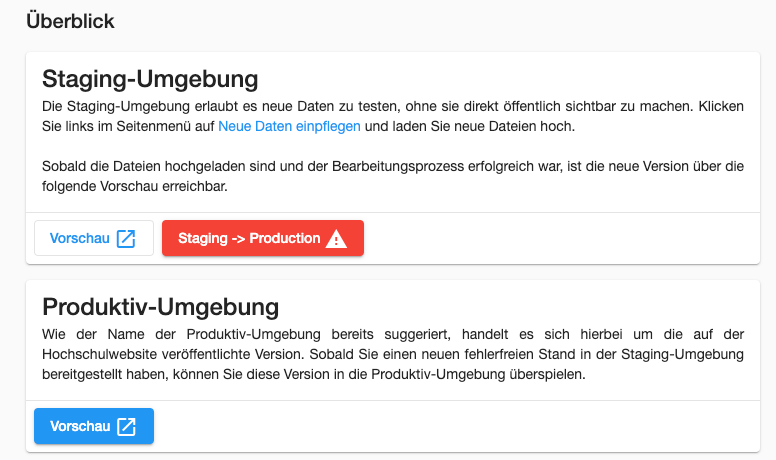
\includegraphics[width=0.8\textwidth]{adminui-overview-1}
    \caption{Admin UI: Überblick}
    \bildquelle{Eigene Darstellung}
    \label{fig:adminui-overview-1}
\end{figure}

Direkt unterhalb befinden sich auf der Übersichtsseite außerdem zwei Architekturgrafiken, die dem Benutzer die Struktur von StudyMap und die damit verbundene Datensicherung über die Versionshistorie verdeutlichen sollen.

\paragraph*{Neue Daten einpflegen}
Auf der Seite zur Eingabe neuer Daten gibt es die Möglichkeit, zwei CSV-Dateien vom Computer auszuwählen (siehe \autoref{fig:adminui-new-data-1}). Dies ist die Datenquelle, die in \autoref{sec:datenquelle} beschrieben wurde. Sie enthält alle Studiengänge und die dazugehörigen Werte der Inhaltskategorien. Die zweite Datei enthält die Abkürzungen der Fakultäten und den entsprechenden Farbcodes, um die Bubbles entsprechend den Fakultäten einzufärben.

\begin{figure}[H]
    \centering
    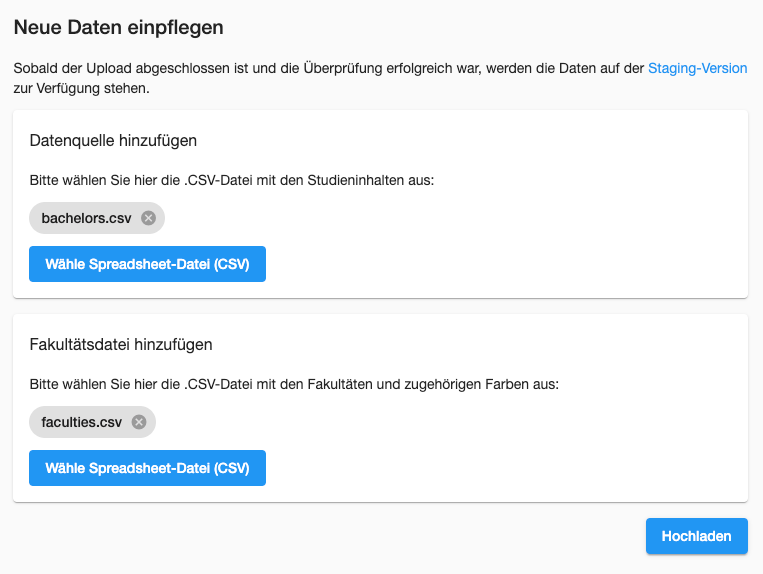
\includegraphics[width=0.8\textwidth]{adminui-new-data-1}
    \caption{Admin UI: Neue Daten einpflegen}
    \bildquelle{Eigene Darstellung}
    \label{fig:adminui-new-data-1}
\end{figure}

Nach der Auswahl der beiden Dateien können diese mithilfe der Schaltfläche \glqq Hochladen\grqq{} hochgeladen und verarbeitet werden. Sobald das Hochladen abgeschlossen ist, beginnt die Verarbeitung der Dateien. Anschließend erscheint ein Dialogfeld mit der Antwort des Servers (siehe \autoref{fig:adminui-new-data-2}).

\begin{figure}[H]
    \centering
    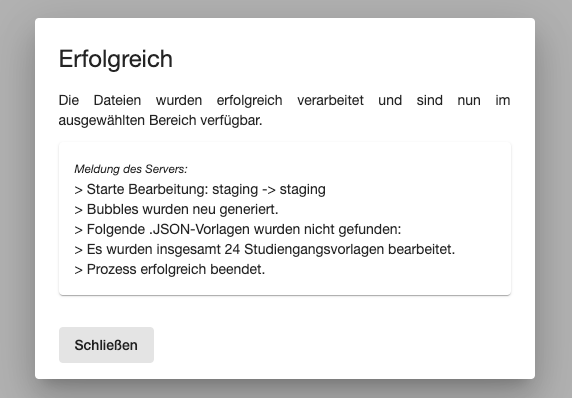
\includegraphics[width=0.5\textwidth]{adminui-new-data-2}
    \caption{Admin UI: Neue Daten einpflegen - Ergebnisdialog}
    \bildquelle{Eigene Darstellung}
    \label{fig:adminui-new-data-2}
\end{figure}

\paragraph*{Neue Daten einpflegen}
\begin{figure}[H]
    \centering
    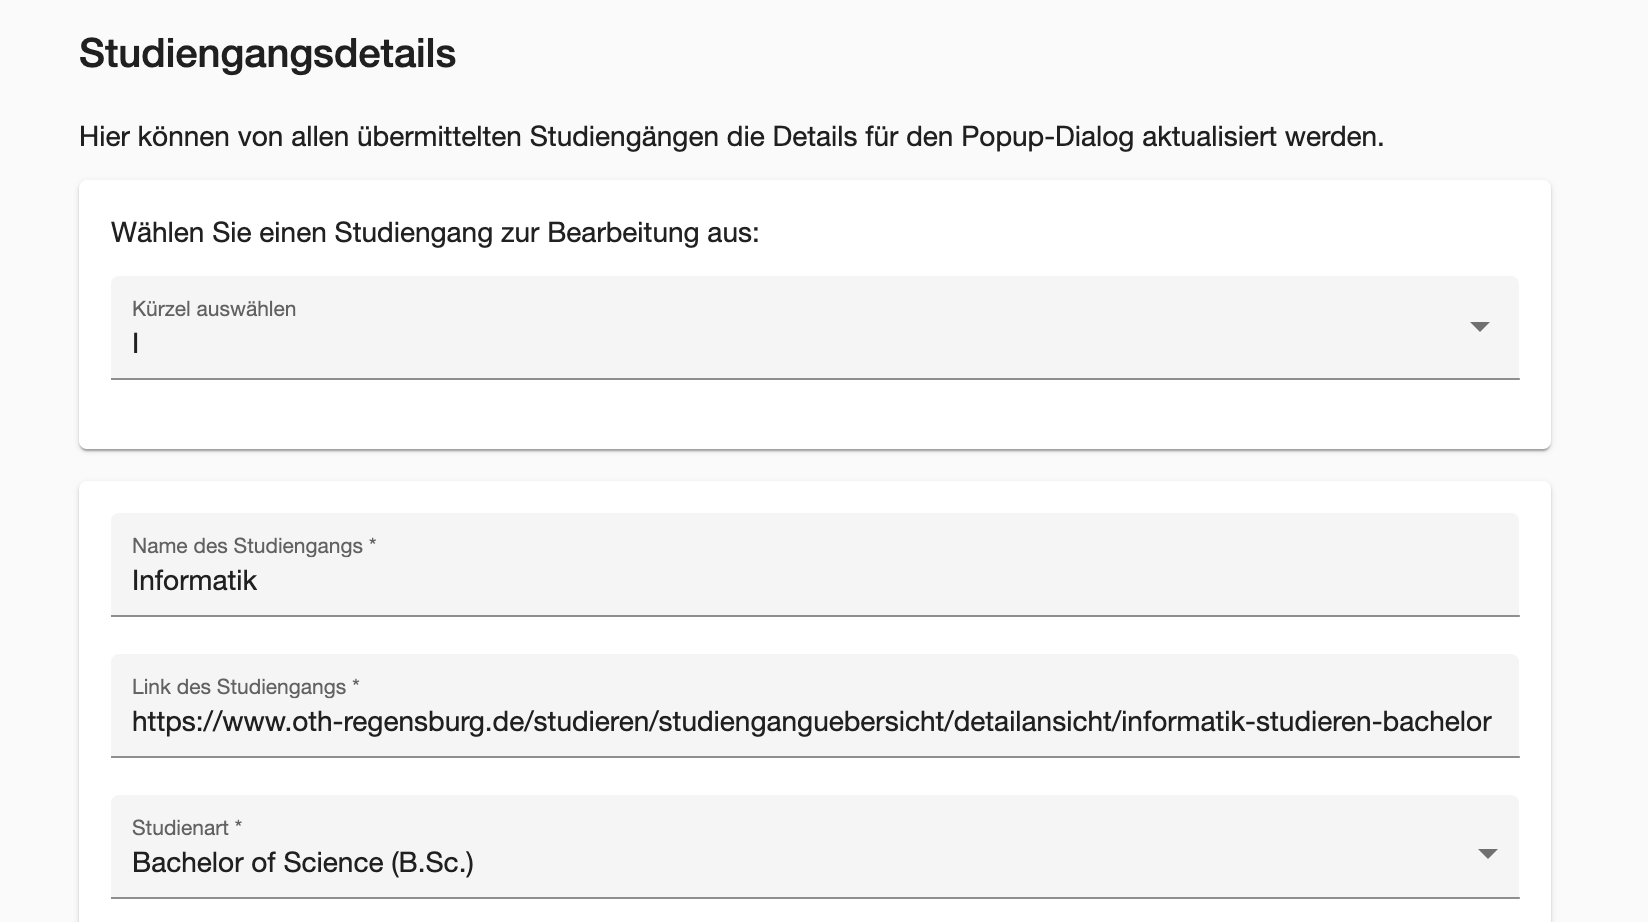
\includegraphics[width=0.8\textwidth]{adminui-details-1}
    \caption{Admin UI: Studiengangsdetails verwalten (Ausschnitt)}
    \bildquelle{Eigene Darstellung}
    \label{fig:adminui-details-1}
\end{figure}

Sobald die Dateien hochgeladen wurden, wird für jeden Studiengang eine Studiengangsdetails-Datei angelegt. Diese kann mithilfe eines grafischen Formulars in der Administrationsoberfläche bearbeitet werden. \autoref{fig:adminui-details-1} zeigt einen Ausschnitt dieses Formulars. Zunächst muss der zu bearbeitende Studiengang oben im Auswahlfenster ausgewählt werden. Anschließend können alle statischen Inhalte des Popups, das sich beim Klick auf eine Bubble in der StudyMap öffnet, bearbeitet werden. Die Liste der regionalen Unternehmen, die Karrieremöglichkeiten für diesen Studiengang anbieten, ist ebenfalls in das zu bearbeitende Formular integriert.

\newpage
\subsection{Softwarearchitektur}
Das Gesamtbild StudyMap setzt sich aus den vorher genauer erläuterten Komponenten REST-API, PixiJS, Python-Backend und Node.js als Webserver für alle Dienste zusammen. Dieses Kapitel beschäftigt sich mit der Architektur und der Kommunikation der einzelnen Komponenten untereinander.

Obwohl die Softwarearchitektur erst in den letzten 30 Jahren an Bedeutung gewonnen hat, ist sie ein fester Bestandteil der Softwareentwicklung und definiert wesentliche tragende Säulen des Produkts. Dabei geht die Softwarearchitektur nicht auf die internen Details einer bestimmten Komponente ein. \parencite{vogel_einleitung_2009} Sie soll komplexe Zusammenhänge übersichtlich darstellen und Fragen wie folgende beantworten:
\begin{itemize}
    \item Wie hängen die Systembausteine miteinander zusammen?
    \item Welche Schnittstellen haben die Komponenten?
    \item Worauf sind Strukturierungen und Entscheidungen zurückzuführen?
\end{itemize}

Für StudyMap ist eine Darstellung der Softwarearchitektur aus mehreren Gründen essentiell.

\paragraph*{Grund 1: Komplexität}
Die Komplexität der Software wird übersichtlicher dargestellt. Da bei der Verwendung mehrerer Programmiersprachen wie JavaScript, TypeScript und Python schnell die Übersicht über die einzelnen Komponenten verloren gehen kann, besteht die Gefahr, ineffizienten oder im schlimmsten Fall fehlerhaften Code zu produzieren. Ein weiterer Grund ist die Einarbeitung zukünftiger Entwickler.

\paragraph*{Grund 2: Einarbeitung}
Da StudyMap im Rahmen dieser Masterarbeit entsteht, ist es abzusehen, dass es immer wieder wechselnde Stakeholder und Weiterentwickler für das Projekt geben wird. Diese müssen zwangsläufig eingearbeitet werden und das Gesamtprojekt verstehen. Ein Entwickler, dem der gesamte Workspace ohne Strukturgrafik mit vier miteinander kommunizierenden Projekten präsentiert wird, könnte anfangs überfordert sein. Deshalb dient die Softwarearchitektur der effizienten Einarbeitung.

\paragraph*{Grund 3: Sicherheit}
Schließlich ist die Strukturgrafik für die Sicherheit der Hochschule von Bedeutung. StudyMap enthält einen geschützten Administrationsbereich. Es sollte im Vorfeld genau festgelegt werden, dass z.B. der Administrationsbereich nur über das VPN der Hochschule erreichbar ist, um die Wahrscheinlichkeit eines Hackerangriffs zu reduzieren. Solche Beziehungen lassen sich mithilfe der Definition einer Softwarearchitektur präzise festlegen. Außerdem benötigt man diese Darstellung explizit an der OTH-Regensburg, um einen Server vom Rechenzentrum für das Hosting von StudyMap zu erhalten. Weitere Informationen dazu finden Sie im \autoref{sec:deployment}.

\begin{figure}[H]
    \centering
    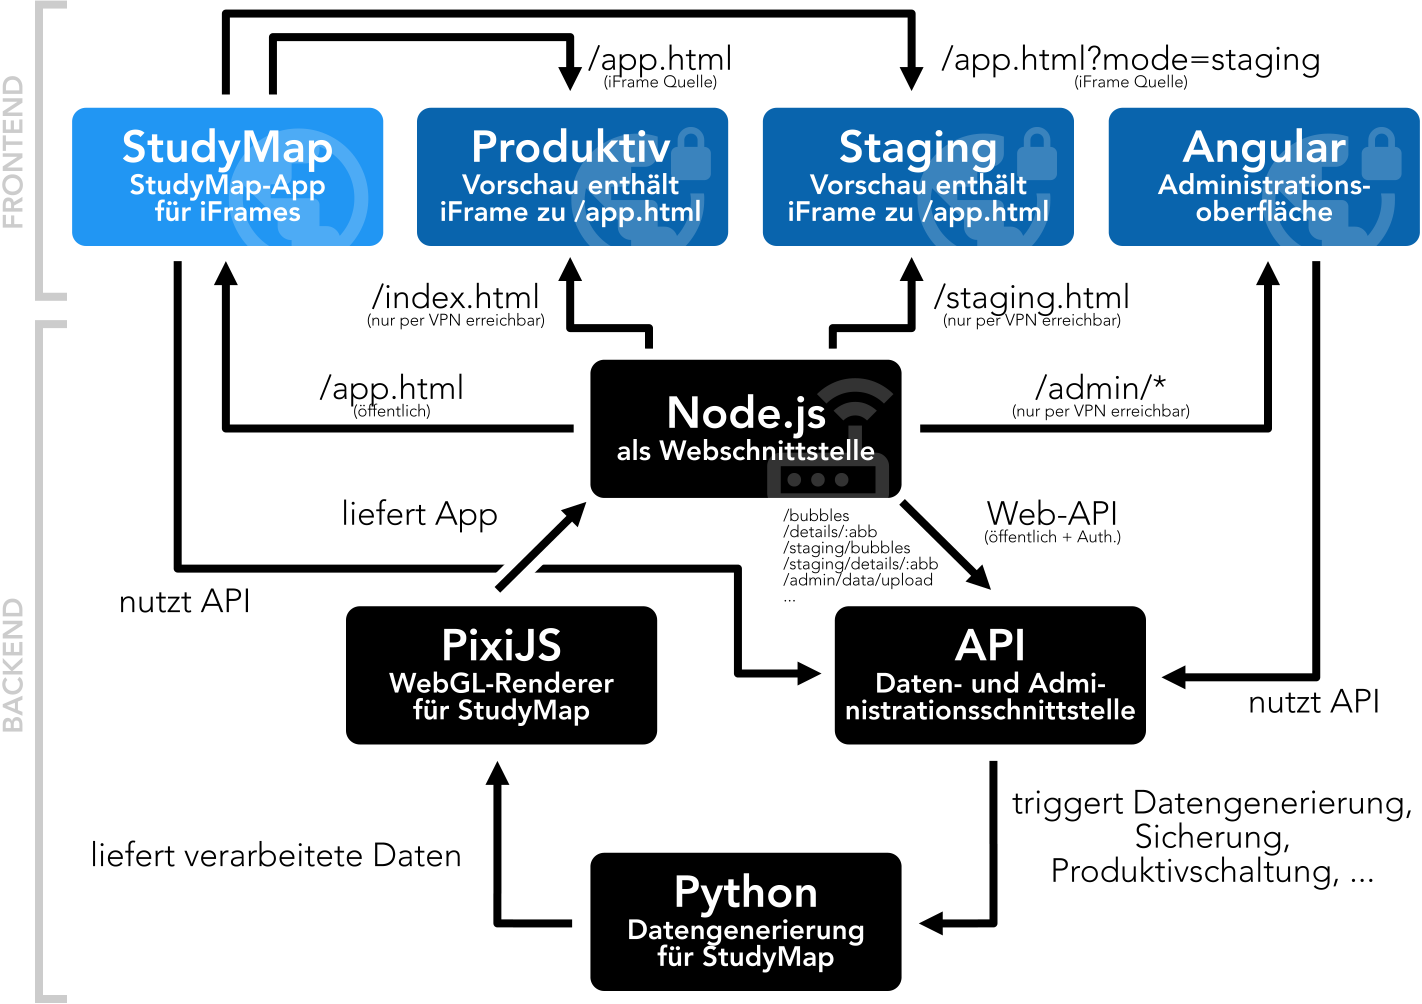
\includegraphics[width=\textwidth]{architecture}
    \caption{Softwarearchitektur von StudyMap}
    \bildquelle{Eigene Darstellung}
    \label{fig:studymap-architecture}
\end{figure}

\autoref{fig:studymap-architecture} zeigt die Softwarearchitektur von StudyMap. Die Anwendungskomponenten werden durch abgerundete Rechtecke beschrieben. Die schwarzen Rechtecke repräsentieren die Backend-Komponenten, während die blauen die Frontend-Komponenten darstellen. Die Beziehungen zwischen den Komponenten werden durch Pfeile visualisiert.

\subsubsection{Frontend-Komponenten}\label{sec:frontend-komponenten}
Alle Frontend-Komponenten werden über die Node.js-Webschnittstelle gehostet. Node.js wird mithilfe von Express genutzt, um neben der in \autoref{sec:node-js-restapi} erläuterten REST-API auch die restlichen Webseiten wie die Anwendung selbst und die Administrationsoberfläche bereitzustellen. Die Frontend-Komponenten in Dunkelblau sind ausschließlich über eine aktive VPN-Verbindung der Hochschule erreichbar.

\paragraph*{StudyMap}
Die Frontend-Komponente StudyMap ist das fertige Produkt. Die StudyMap-App besteht aus dem PixiJS-Canvas, der mit Bootstrap verbunden ist, um den Studiengangsdetails-Dialog anzuzeigen (siehe \autoref{fig:mockup-bubbles-popup}). Es handelt sich um eine reine Web-App ohne weitere Design-Elemente rund um den Canvas herum. Der Grund dafür ist, dass die StudyMap-Anwendung als iFrame in die Website der Hochschule eingebunden wird, d.h. die Anwendung muss den gesamten Bildschirminhalt ausfüllen, damit sich der iFrame später nahtlos in die Hochschulwebsite einfügt. Das HTML-Element iFrame erlaubt die Einbindung externer Webseiten in eine Seite. Ein klassisches Beispiel hierfür ist die Einbindung einer Anfahrtskarte eines Kartendienstleisters wie OpenStreetMap auf Unternehmenswebsites. \parencite{mozilla_corporation_iframe_2024} In dieser Arbeit wird der Studiengangsfinder in die Hochschulwebsite eingebettet.

\noindent
Webschnittstelle: \code{/app.html}

\paragraph*{Produktiv}
Wie in \autoref{fig:studymap-architecture} dargestellt, ist die Produktiv-Schnittstelle eine HTML-Website, die die StudyMap-App per iFrame einbettet.  Das Bestreben ist es, ein möglichst realitätsnahes Produktivsystem nachzubilden, weshalb die Produktivkomponente einen ähnlich breiten Platz für den iFrame verwendet, wie er auch auf der Website der OTH zur Verfügung steht. Die Produktivkomponente ist ausschließlich über das VPN der Hochschule erreichbar.

\noindent
Webschnittstelle: \code{/index.html}

\paragraph*{Staging}
Die Staging-Umgebung ist nahezu identisch mit der Produktivumgebung. Der Unterschied zwischen den beiden besteht darin, dass hier zusätzlich der Queryparameter \code{?mode=staging} an die Quelladresse des iFrames (\code{/app.html}) angehängt wird. Anhand dieses Parameters erkennt PixiJS, dass es sich um eine Testumgebung handelt und holt sich die Daten aus dem Staging-Bereich des Backends.

Mit dieser Testseite können neue Daten vor der Veröffentlichung getestet und optimiert werden. Die Staging-Komponente ist ebenfalls nur per VPN erreichbar.

\noindent
Webschnittstelle: \code{/staging.html}

\paragraph*{Angular}\label{paragraph:angular-basic-auth}
Die vierte und letzte Komponente ist die Angular-Administrationsoberfläche. Offensichtlich darf vor allem dieser Teil der Anwendung nur über eine authentifizierte VPN-Verbindung erreichbar sein. Der gesamte Administrationsbereich ist außerdem durch eine Basic-Auth-Middleware geschützt.

\begin{figure}[H]
    \centering
    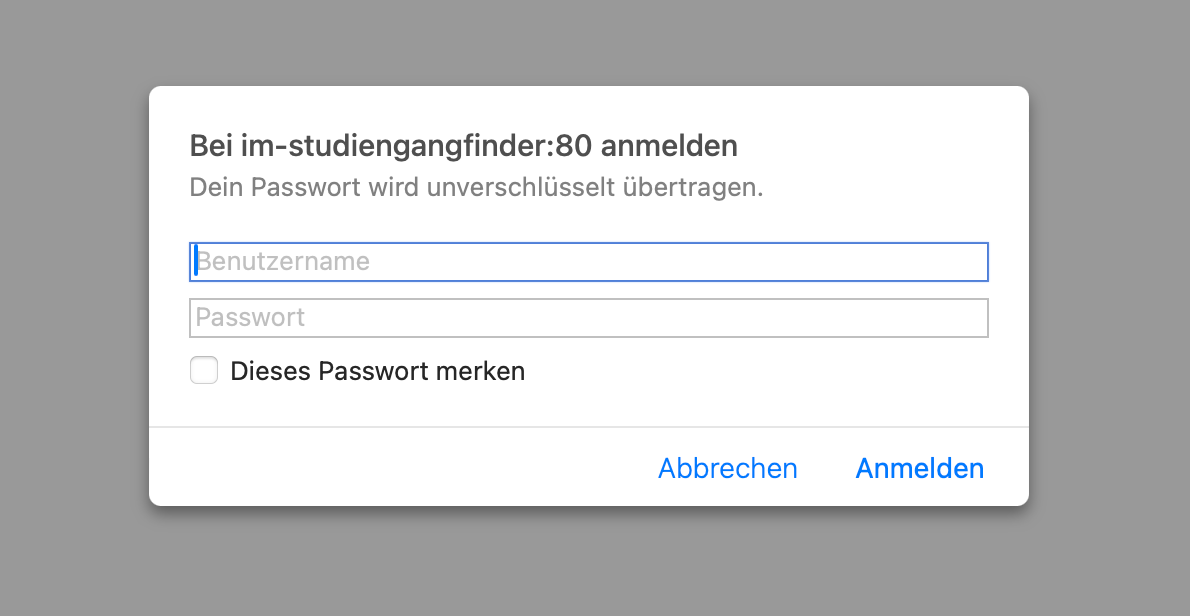
\includegraphics[width=0.6\textwidth]{basic-auth}
    \caption{Basic-Auth-Middleware von StudyMap}
    \bildquelle{Eigene Darstellung}
    \label{fig:basic-auth}
\end{figure}

Basic-Auth ist ein allgemeines Authentifizierungsframework, das standardmäßig in der HTTP-Definition enthalten ist. \parencite{mozilla_corporation_http_2023} Es wird von allen gängigen Browsern unterstützt und erfordert nicht die Implementierung eines eigenen Authentifizierungsverfahrens. \parencite{fyrd_headers_2024} Wenn ein Webserver, in diesem Fall das Node.js-Webinterface, eine Authentifizierung anfordert, können Browser diese Anforderung verarbeiten und ein generisches Anmeldeformular anzeigen (siehe \autoref{fig:basic-auth}).

In \autoref{fig:basic-auth} fehlt ein SSL-Zertifikat, wodurch keine verschlüsselte Verbindung möglich ist. SSL-Zertifikate sind kleine Datendateien, die kryptografische Schlüssel digital an eine Organisation binden. Somit können HTTPS-Verbindungen genutzt werden, welche wiederum die Browserverbindungen verschlüsseln und somit auch die eingegebenen Daten vor Mitlesern schützen. \parencite{globalsign_was_2023}

Daher wird auch eine Basic-Auth-Authentifizierung als unsicher eingestuft, wenn kein SSL-Zertifikat vorhanden ist. Um die Sicherheitsbedenken von StudyMap auszuschließen, sollte in Zukunft die Authentifizierung über einen externen Authentifizierungsprovider der Hochschule erfolgen. Dadurch muss StudyMap keine Anmeldedaten speichern und es besteht kein Risiko mehr für einen Hackangriff.

Nach Abschluss der Authentifizierung kann der Nutzer die Administrationsoberfläche nutzen. Die Web-App dient der Verwaltung der Anwendung und ihrer Daten. Zu diesem Zweck werden verschiedene HTTP-Anfragen verwendet, mit denen die REST-API aufgerufen wird.

\noindent
Webschnittstelle: \code{/admin/*}

\subsubsection{Backend-Komponenten}
Das Backend der Softwarearchitektur besteht neben der bereits im \autoref{sec:frontend-komponenten} erläuterten Node.js Webschnittstelle aus drei weiteren Komponenten: \begin{enumerate}
    \item PixiJS: WebGL-Renderer für StudyMap
    \item API: Daten- und Administrationsschnittstelle
    \item Python: Datengenerierung für StudyMap
\end{enumerate}

\paragraph*{PixiJS}
Das PixiJS-Projekt ist ein eigenständiges JavaScript-Projekt, das die vorher erläuterte HTML-Datei \code{app.html} für die Frontend-Komponenten generiert und darin den WebGL-Renderer für StudyMap einbindet. Dieses Projekt enthält ebenfalls HTTP-Anfragen zur REST-API, um die Daten der Studiengänge abzurufen. Es ist jedoch wichtig zu beachten, dass diese Anfragen durch den Browser-Client bzw. die Frontend-Komponenten aufgerufen werden und somit streng genommen kein Teil der Backend-Komponente ist.

\paragraph*{API}
Die API (Application Programming Interface) bietet nicht nur die Lieferung von Positions- und Studiengangsdetailsdaten, sondern auch die Möglichkeit, die im Server gespeicherten Daten zu verwalten und zu ändern (siehe \autoref{sec:node-js-restapi}). Aus diesem Grund ist die Administrationsoberfläche sowie die StudyMap-App selbst mit der API verbunden.

Wenn jemand in der Administrationsoberfläche neue Dateien hochlädt, wird eine Anfrage an die API gesendet. Diese speichert die Dateien an der richtigen Stelle und löst schließlich die Generierung neuer Positionsdaten durch eine Anfrage an die Python-Komponente aus. Die Python-Komponente ist folglich ebenfalls mit der API angebunden.

\paragraph*{Python}
Die Python-Komponente hat im Wesentlichen nur eine Verbindung zu einer anderen Komponente, nämlich zur REST-API, die Python aufruft. Die Python-Komponente enthält die Logik für die Generierung der auszuliefernden Dateien sowie für die Datensicherung. Das Python-Skript implementiert den MDS-Algorithmus zur Berechnung der genauen Positionsdaten anhand der Ähnlichkeiten zwischen den Studiengängen. Beide Anwendungsfälle werden durch die Kommandozeile der REST-API getriggert.

Es besteht eine weitere implizite Verbindung zwischen PixiJS und den Daten des Python-Skripts für die Anzeige der Bubbles. Die eigentliche Kommunikation zwischen den Komponenten erfolgt jedoch über die Programmierschnittstelle.

\newpage
\subsection{Software Deployment}\label{sec:deployment}
Nachdem die Softwarearchitektur geklärt und implementiert wurde, folgt in diesem Abschnitt das Deployment. Software Deployment (Softwareverteilung) bezeichnet den Prozess der Konfiguration und Installation auf dem Zielserver. Dieser Prozess besteht in der Regel aus mehreren Schritten, wie Planung, Design, Testen, Terminplanung und Deployment. \parencite{atera_team_was_2023} Im Falle von StudyMap beschränkt sich der Prozess auf die Schritte: Planung, Testen und Bereitstellung.

\subsubsection{Planung}
Der erste Schritt des Softwareverteilungsprozesses ist die Planung, welcher diverse W-Fragen beantwortet. Es ist beispielsweise wichtig zu berücksichtigen, wie viele Nutzer die Anwendung später haben werden, welche Risiken zu erwarten sind und wie eine Authentifizierung aussehen könnte. \parencite{atera_team_was_2023}

Bei dieser Arbeit waren bereits einige Planungspunkte vorgegeben, da an der Hochschule Regensburg ein spezielles IT-Verfahren zum Schutz der Hochschule eingesetzt wird. Um das Projekt StudyMap auch nach der Übergabe der Masterarbeit weiterführen zu können, wurde eine gewisse Normbeschreibung erstellt. In der folgenden Liste sind einige ausformulierte Punkte und Details des Planungsschrittes aufgeführt.

\paragraph*{Wer sind die Verantwortlichen für die Software?}
Die Verfahrensverantwortliche Person ist Prof. Dr.-Ing. Birgit Rösel, Vizepräsidentin der OTH-Regensburg. Sie hat den Bedarf der Studienorientierung erkannt und das Projekt initiiert. Während der Entwicklung ist Andreas Huber, der Autor dieser Arbeit, die technisch verantwortliche Person.

Die technisch Verantwortliche Person ist für die Wartung und das Patchmanagement zuständig. Es ist erforderlich, alle Pakete und Programme auf dem neuesten Stand zu halten, um die Wahrscheinlichkeit eines Hackerangriffs zu minimieren. Nach Abgabe dieser Arbeit wird das Amt an eine zum Zeitpunkt des Schreibens noch unbekannte Person übertragen.

\paragraph*{Wie viele Benutzer wird die Anwendung haben?}
Diese Frage ist insbesondere für die Leistung und die benötigten Serverressourcen von Bedeutung. Zum Zeitpunkt der Entwicklung liegen keine konkreten Besucherzahlen vor. Die Softwarearchitektur ist jedoch so geplant, dass die beschriebene REST-API lediglich .json-Dateien liest und zurückgibt - dies erfordert wenig Rechen- und Netzwerkleistung. Außerdem wird die interaktive Grafik clientseitig berechnet, also auf dem Gerät des Benutzers.

Aus den genannten Gründen wird ein leistungsschwacher virtueller Server mit den folgenden Spezifikationen vom Rechenzentrum angefordert:
\begin{itemize}
    \item Prozessorkerne: 1 Kern
    \item Arbeitsspeicher: 8 GB
    \item Festplattenspeicher: 100 GB
    \item Betriebssystem: Debian 12
\end{itemize}

\paragraph*{Wie kritisch ist ein Ausfall des Systems?}
Ein Ausfall des Projekts ist weniger schwerwiegend, da es sich nur um ein optionales Feature der Hochschulwebsite handelt. Aus diesem Grund reicht es, das System innerhalb einer Wochenfrist wiederherzustellen. Darüber hinaus wird die Gesamtfunktion nicht ständig überwacht.

\paragraph*{Werden personenbezogene Daten gespeichert?}
Um rechtliche Fragen abzusichern, muss geklärt werden, ob im Falle eines Angriffs das Risiko besteht, persönliche Informationen zu verlieren. Daher ist es wichtig zu ermitteln, ob personenbezogene Daten gespeichert werden. StudyMap ist eine unabhängige Software, die Informationen über Studiengänge enthält, welche bereits veröffentlicht wurden. Das Hochladen und Speichern dieser Informationen in StudyMap durch eine verantwortliche Person ist ohne die Eingabe personenbezogener Daten möglich.

Aus diesem Grund gehören die verarbeiteten Informationen zur Hochschul-Informationsklasse \glqq V0 - öffentlich\grqq{}. Dies bedeutet, dass keine der verarbeiteten oder gespeicherten Informationen im Falle eines Diebstahls als kritisch eingestuft werden würde.

\paragraph*{Wie wird sichergestellt, dass gewisse Bereiche nur per VPN zugänglich sind?}
% TODO

\paragraph*{Wie wird die Authentifizierung sichergestellt?}
Wie bereits in \autoref{paragraph:angular-basic-auth} erläutert, wird die Authentifizierung mittels einer Middleware im Webserver sichergestellt. Zudem wird vom Rechenzentrum eine separate IP-Adresse angefordert, um den Zugriff auf bestimmte Bereiche, wie beispielsweise den Administrationsbereich, nur mit aktiver VPN-Verbindung zu ermöglichen. % TODO: Wirklich so?

\paragraph*{Welche Rollen sind vorgesehen?}
In engem Zusammenhang mit der Frage der Authentifizierung steht die Frage, welche Rollen in der Anwendung vorgesehen sind. Im Studiengangsfinder gibt es lediglich zwei Rollen:
\begin{enumerate}
    \item Administrator
    \item Besucher
\end{enumerate}
Die Besucher-Identität hat ausschließlich Zugriff auf die Frontend-Komponente \code{app.html}, welche die interaktive Grafik enthält. Eine Authentifizierung ist nicht erforderlich. Die Administrator-Identität hingegen hat Zugriff auf alle weiteren Frontend-Komponenten und kann somit die gespeicherten Daten verwalten.

\paragraph*{Wer kümmert sich um die Aktualität der Daten?}
Frau Rösel ist für die Aktualität der Daten verantwortlich, während der Entwicklung und nach der Übergabe des Projekts für einen unbestimmten Zeitraum. Nach Abgabe dieser Arbeit wird Andreas Huber, der technische Verantwortliche, Sie unverzüglich über den Prozess der Datenverwaltung durch die Administrationsoberfläche instruieren. Wer die Daten langfristig pflegt bleibt noch offen.

\paragraph*{Werden regelmäßige System- und Datensicherungen duchgeführt?}
Der Server von StudyMap befindet sich im zentralen Serverraum des Rechenzentrums der OTH-Regensburg. Dadurch wird sichergestellt, dass die Organisation täglich eine Systemsicherung durchführt.

Eine Datensicherung erfolgt nur beim Überführen eines Datenstands von Staging in die Produktivumgebung. Wie bereits beschrieben, speichert StudyMap immer die letzten zehn Produktivstände, um im Falle von korrupten Daten eine Datensicherung wiederherstellen zu können. Es gibt keine zeitgesteuerten Intervall-Datensicherungen.

\paragraph*{Was ist der Ablauf bei einem eintretenden Sicherheitsvorfall?}
Sollte es zu einer Kompromittierung des Servers kommen, muss die verantwortliche Person sofort Kontakt mit security@oth-regensburg.de aufnehmen und diese über den Vorfall informieren.

\paragraph*{Wer stellt ein SSL-Zertifikat zur verschlüsselten Übertragung der Daten?}
Damit die Verbindung zu StudyMap funktioniert, wird ein SSL-Zertifikat sowohl für die internen (VPN-Bereich) als auch für die externen Anfragen benötigt.

Wenn kein SSL-Zertifikat auf dem Webserver installiert ist, werden die Login-Anfragen unverschlüsselt verschickt. Ein Angreifer könnte dadurch die Zugangsdaten mitlesen und daraus einen weiteren Hackangriff starten.

Obwohl keine sicherheitsrelevanten Informationen beim Öffnen der Besucheransicht geteilt werden, benötigt StudyMap auch für den öffentlichen Bereich ein SSL-Zertifikat. Der Grund dafür ist, dass die Hochschulwebsite eine https-Verbindung erzwingt. Moderne Browser erlauben es nicht, einen iFrame mit einer unverschlüsselten Website auf einer verschlüsselten Website einzubinden. \parencite{vyas_mixed_2013}

\subsubsection{Testen}
In dieser Phase des Deployment-Prozesses wird eine Testumgebung erstellt, um zu überprüfen, ob alles wie vorgesehen funktioniert. Ziel ist die Schaffung einer möglichst realitätsnahen Umgebung, damit der endgültige Prozess der Bereitstellung auf dem Server der Universität mit möglichst wenigen unvorhersehbaren Komplikationen verbunden ist.

\paragraph*{Verwendung von Docker zur Auslieferung}
StudyMap wird auf dem Produktivserver in einem Docker Container gehostet. Docker ist eine Open-Source-Plattform zur Erstellung und Bereitstellung von Anwendungen. Docker arbeitet mit sogenannten Containern, die alle Pakete, benötigten Abhängigkeiten, Werkzeuge und Code enthalten, die für die Ausführung der Software notwendig sind. \parencite{amazon_web_services_inc_was_2023}

Docker Container visualisieren das Betriebssystem eines Servers. Jeder Container basiert auf einem Image, wie zum Beispiel einem Linux-Derivat. Auf diesem werden alle benötigten Pakete installiert. Docker-Images sind leichtgewichtige und dennoch effiziente eigenständige Pakete, da sie denselben System-Kernel verwenden und somit nicht für jede Anwendung ein vollständiges Betriebssystem benötigen. \parencite{docker_inc_what_2024}

Neben der Effizienz ist auch die Sicherheit ein zusätzlicher Pluspunkt. Anwendungen, die in Containern ausgeführt werden, sind voneinander isoliert und erlauben nur die Kommunikation, die durch die Konfiguration erlaubt ist. \parencite{docker_inc_what_2024}

Ein weiterer Vorteil ist die Möglichkeit, Docker Container schnell von einem Server auf einen anderen zu übertragen, ohne den Server für die neue Anwendung konfigurieren zu müssen. Der Docker Container enthält alle notwendigen Netzwerk- und Software-Konfigurationen, die auf dem Zielserver unter Umständen nicht vorhanden sind. Dadurch können Probleme durch beispielsweise unterschiedliche Softwareversionen vermieden werden. Unterschiedliche Anwendungen benötigen oft unterschiedliche Paketversionen, wie zum Beispiel Python oder Python3. Solche Situationen können zu aufwendigen Konfigurationsprozessen führen, während mit Docker alles isoliert in einem Container genau für die Anwendung enthalten ist. \parencite{amazon_web_services_inc_was_2023}

\paragraph*{Docker-Image für StudyMap}
Um StudyMap in einem Docker Container auszuführen, wird ein Docker-Image benötigt, das alle Komponenten der Softwarearchitektur enthält. Für die Entwicklung dieses Images wird als Basisimage ein Node.js-Image verwendet. Auf diesem Basisimage werden alle Konfigurationen und zusätzlichen Komponenten festgelegt, die dann beim Starten des Containers automatisch installiert werden. Da Node.js als Webschnittstelle für den Studiengangsfinder dient, bildet es die ideale Basis für das Docker-Image. Nachfolgend ist das für StudyMap entwickelte Dockerfile abgebildet:

\noindent
\begin{minipage}{\linewidth}
\begin{lstlisting}[style=Python]
# Node version 18 as base image
FROM node:18

# Install python
RUN apt-get update && apt-get install -y python3 python3-pip

# Set work directory
WORKDIR /app

# Copy dir
COPY . .

# Install dependencies
RUN npm install
WORKDIR /app/admin
RUN npm install
RUN npm run build
WORKDIR /app/frontend
RUN npm install
RUN npm run build:prod
WORKDIR /app/backend/generator
RUN pip3 install -r requirements.txt --break-system-packages
WORKDIR /app

# Expose ports
EXPOSE 8080

# Launch
CMD ["npm", "start"]
\end{lstlisting}
\end{minipage}


Docker kann mithilfe einer Dockerfile in Form eines Textdokuments ein Image erstellen. In der Dockerfile befinden sich alle Befehle, um ein Image zusammenzustellen. \parencite{docker_inc_dockerfile_2024} Das für StudyMap entwickelte Dockerfile beginnt mit dem Befehl \code{FROM node:18}. Dies bedeutet, dass das Base Image \code{node} in Version 18 als Grundlage für dieses Image verwendet wird. Eine Dockerfile, die lediglich die erste Zeile zur Festlegung des Base Images enthält, würde dementsprechend ein bestehendes Image ohne Veränderung 1:1 kopieren. \parencite{the_nodejs_docker_team_node_2024}

In Zeile fünf wird die Anweisung gegeben, die Paketlisten des Systems zu aktualisieren und \code{python3} sowie \code{python3-pip} zu installieren, den offiziellen Paketmanager der Programmiersprache Python. \parencite{the_pip_developers_pip_2024} Mit dem \code{RUN}-Befehl in Dockerfiles kann der Container angewiesen werden, diese Anweisung in der Befehlszeile des Containers auszuführen. Das Node-Image basiert auf dem Alpine-Linux-Image, welches das Linux-Paketverwaltungswerkzeug APT (Advanced Packaging Tool) enthält. \parencite{the_nodejs_docker_team_node_2024} Dieses Werkzeug ermöglicht es, Pakete, wie z.B. \code{python3}, auf einfache Art und Weise per Kommandozeile mit dem Befehl \code{apt-get install} zu installieren. \parencite{canonical_ltd_ubuntu_package_2024}

In Zeile acht wird das Arbeitsverzeichnis des Containers auf den Pfad \code{/app} gesetzt, indem der Befehl \code{WORKDIR} verwendet wird. Alle folgenden Befehle werden relativ zu diesem Ordner ausgeführt. Falls der angegebene Pfad nicht vorhanden ist, wird Docker ihn im Dateisystem des Containers erstellen. \parencite{docker_inc_dockerfile_2024}

Mit dem gegebenen \code{COPY}-Befehl wird der gesamte Inhalt des Ordners, in dem sich die Dockerfile befindet, in den Ordner kopiert, in dem sich der Container gerade befindet. \parencite{docker_inc_dockerfile_2024} Die Dockerfile befindet sich im äußersten Verzeichnis des StudyMap-Git-Repositorys. Das bedeutet, dass alle Dateien und Unterordner des Studiengangsfinders in den Container kopiert werden. Nachdem das \code{WORKDIR} auf \code{/app} gesetzt wurde, werden alle Dateien dementsprechend nach \code{/app} kopiert.

Zeilen 14 bis 23 installieren alle Abhängigkeiten der einzelnen Subprojekte und kompilieren die Dateien zu ausführbaren Anwendungen. In Zeile 14 wird eine Version der Node.js-Webschnittstelle und REST-API erstellt. Anschließend wird in Zeile 15 das Arbeitsverzeichnis auf den Subordner der Administrationsoberfläche gesetzt und mit \code{RUN npm install} und \code{RUN npm build} dessen Abhängigkeiten installiert und kompiliert. Schließlich werden in den Zeilen 18 bis 20 des PixiJS-Projekts dieselben Schritte durchgeführt. Abschließend werden die Python-Abhängigkeiten mit dem bereits vorgestellten Paketmanager pip3 und einer Abhängigkeitsliste im Unterordner \code{requirements.txt} installiert. Python benötigt keinen Build-Prozess, da das Skript zur Laufzeit von der Python-Engine gelesen und ausgeführt wird. Zum Schluss wird in Zeile 23 das Arbeitsverzeichnis auf \code{/app} zurückgesetzt.

In Zeile 26 wird mit dem Kommando \code{EXPOSE 8080} Docker darüber informiert, dass der Port 8080 für die Netzwerkkommunikation genutzt werden soll. Ein Netzwerkport ist eine definierte Nummer, die die Kommunikation für einen bestimmten Dienst empfängt oder überträgt. \parencite{wright_was_2022} Ein Beispiel aus dem Alltag wäre die Wohnungsnummer in einem Mehrparteienhaus, damit die Post den Brief zur richtigen Wohnung innerhalb des Hauses zustellen kann. Der \code{EXPOSE}-Befehl informiert lediglich über den Port, schaltet ihn jedoch nicht frei. Um den Port freizugeben, muss beim Start des Containers der Parameter \code{-p} für Port angegeben werden. \parencite{docker_inc_dockerfile_2024}

Die letzte Zeile enthält lediglich den Startbefehl für das Node.js Projekt, welches anschließend alle weiteren Projekte hostet. Wenn der Container gestartet wird, wird der Kommandozeilenbefehl ausgeführt, der mit dem \code{CMD}-Befehl definiert wurde. Aus diesem Grund darf es im Dockerfile auch nur einen \code{CMD}-Befehl geben. \parencite{docker_inc_dockerfile_2024}

Um das Docker-Image mithilfe des Dockerfiles zu bauen und auszuführen, müssen nun folgende zwei Befehle in der Kommandozeile ausgeführt werden:
\begin{lstlisting}[style=Python]
docker build -t studymap .
docker run -p 8080:8080 studymap
\end{lstlisting}

Der erste Befehl führt den Build-Prozess unter Verwendung der Dockerfile aus, die sich im aktuellen Verzeichnis befindet, und gibt dem daraus entstehenden Image den Namen \code{studymap}. Der zweite Befehl erstellt einen Container mit dem gerade erstellten Image und leitet den Port 8080 aus dem Container auf den Port 8080 des Betriebssystems des Servers weiter.

\paragraph*{Persistierung der Daten durch Docker Volumes und Docker Compose}
Wie bereits erläutert, werden in StudyMap Dateien von außen in den Container hochgeladen und verarbeitet. Wenn ein Docker Container jedoch neu gestartet wird, wird sein Zustand zurückgesetzt. Das bedeutet, dass alle veränderten Dateien wieder im Originalzustand sind und alle neu hinzugefügten Dateien gelöscht werden. Aus diesem Grund ist die Verwendung von Docker Volumes zur Persistenz über einen Neustart hinaus notwendig.

Docker Volumes ermöglichen es, Daten von Containern betriebssystemunabhängig zu persistieren. Sie ermöglichen die Erstellung von Container-übergreifendem Speicher und sind dabei deutlich effizienter und performanter als Bind-Mounts eines Betriebssystems. \parencite{docker_inc_volumes_0000}

Für die Verwendung von Docker Volumes muss der Kommandozeilenbefehl zum Starten des Containers angepasst bzw. deutlich erweitert werden. Eine Alternative hierzu ist die Verwendung von Docker Compose. Docker Compose wurde entwickelt, um mehrere Container effizient zu steuern und eine klare Struktur von vielen Containern zu ermöglichen. Hier gibt es neben den Dockerfiles auch eine \code{docker-compose.yml}-Datei, die alle Informationen zu den Containern bezüglich Netzwerk, Speicher und freizugebenden Ports enthält. Da der Kommandozeilenbefehl zum Starten des StudyMap-Docker Containers aufgrund der Ports und Volumes dokumentiert werden müsste, bietet sich die Verwendung von Docker Compose an. Die benötigten Volumes sowie der freizugebende Port 8080 werden in einer Datei festgehalten. \parencite{docker_inc_docker_0000} Der Administrator kann die StudyMap-Anwendung mit folgenden konsistenten Befehlen verwalten:

\noindent
\begin{minipage}{\linewidth}
\begin{lstlisting}[style=Python]
docker compose up -d        # Startet den Container im Hintergrund (-d)
docker compose down         # Stoppt den Container
docker compose restart      # Startet den Container neu
\end{lstlisting}
\end{minipage}

Die im vorherigen Abschnitt erwähnte Datei \code{docker-compose.yml} sieht für den Studiengangsfinder folgendermaßen aus:
\begin{lstlisting}[style=Python]
version: '3.8'

services:
  studymap:
    build: .
    ports:
      - "80:8080"
    volumes:
      - generated-data:/app/gdata
      - input-files:/app/backend/input
    command: ["npm", "start"]

volumes:
  generated-data:
  input-files:
\end{lstlisting}

Die Container-Definition für den Studiengangsfinder befindet sich in den Zeilen vier bis elf. In Zeile vier wird der Name des Containers angegeben und in Zeile fünf das Image, das der Container verwenden soll. In diesem Fall ist das ein wichtiger Punkt, denn die \code{docker-compose.yml}-Datei liegt im selben Verzeichnis wie die Dockerfile. Das bedeutet, dass Docker Compose automatisch die Dockerfile sucht, das Image baut und als Grundlage für den Container verwendet. In Zeile sieben wird der freizugebende Port festgelegt. Der Container gibt den Port 8080 frei, welcher dann auf den Systemport 80 geleitet wird. In Zeile acht bis zehn werden die Volumes festgelegt. Hierbei handelt es sich um zwei Verzeichnisse. Einmal das Verzeichnis, in dem die hochgeladenen Dateien des Benutzers landen und die Datensicherungen angelegt werden, und das zweite Volume, welches die durch den Algorithmus generierten Dateien enthält. Zeile elf ist äquivalent zum \code{CMD}-Befehl aus der bereits erläuterten Dockerfile. In den Zeilen 13 bis 15 werden abschließend die verwendeten Volumes definiert.

Mithilfe der genannten Docker-Dateien kann die Anwendung und das Deployment nun entweder lokal auf dem Entwicklungsrechner oder auf Testservern getestet werden. Nachdem der Container erfolgreich gestartet werden kann, kann mit dem letzten Schritt des Deployments der eigentlichen Bereitstellung begonnen werden.

\subsubsection{Bereitstellung}
Für eine reibungslose und fehlerfreie Bereitstellung auf dem Hochschulserver ist eine sorgfältige Planung erforderlich. Die folgenden Schritte geben eine Reihenfolge und eine Struktur für die Durchführung des Deployments vor:
\begin{enumerate}
    \item Server aktualisieren
    \item Speicherort für StudyMap festlegen
    \item Docker und Docker Compose installieren
    \item StudyMap auf den Server kopieren
    \item Docker Compose ausführen
\end{enumerate}

\paragraph*{1. Server aktualisieren}
Zuerst müssen der Server und seine Paketlisten aktualisiert werden. In Debian kann dies mit den folgenden Befehlen durchgeführt werden:
\begin{lstlisting}[style=Python]
apt-get update
apt-get upgrade
\end{lstlisting}

\paragraph*{2. Speicherort für StudyMap festlegen}
% TODO: Quelle
Es muss anschließend der Speicherort für StudyMap festgelegt werden. Der Standardordner für Docker Container unter Linux ist \code{/var/lib/docker}. Da die Partition auf dem vom Rechenzentrum bereitgestellten Server nur 3,9 Gigabyte Speicherplatz hat, muss auf das Home-Verzeichnis mit 13 Gigabyte ausgewichen werden. Für diese Änderung ist eine Anpassung der Datei \code{/etc/docker/daemon.json} erforderlich:
\begin{lstlisting}[style=Python]
{
    "data-root": "/home/docker-data"
}
\end{lstlisting}

\paragraph*{3. Docker und Docker Compose installieren}
Der nächste Schritt besteht in der Installation der Docker Engine und dem Plugin Docker Compose. Die Pakete hierfür sind nicht in den Standard-Paketlisten von APT enthalten. Aus diesem Grund wird auf der Docker Installationswebsite die Step-by-Step-Anleitung befolgt, um die Paketlisten zu erweitern und Docker schließlich per Paketmanager zu installieren.

\noindent
Offizielle Installationsanleitung für Debian: \url{https://docs.docker.com/engine/install/debian/}

\paragraph*{4. StudyMap auf den Server kopieren}
% TODO: Quelle
Um das Projekt auf den Server zu übertragen, wird das gesamte Git-Repository, einschließlich des Dockerfiles und der \code{docker-compose.yml}-Datei, per SCP auf den Server kopiert. Der Quellcode befindet sich derzeit auf der Plattform GitHub. Es ist möglich, Repositories direkt als .zip-Datei herunterzuladen. Falls es nicht möglich ist, das Repository als .zip-Datei herunterzuladen, kann alternativ das lokale Entwicklungsprojekt als Zip-Datei komprimiert und übertragen werden. In diesem Fall ist es jedoch wichtig, alle Build-Dateien, Bibliotheken und Abhängigkeiten zu entfernen, die sowieso nachinstalliert werden müssen, um unnötig große Datentransfers zu vermeiden.

Anschließend genügt ein Kommandozeilenbefehl, um die Anwendung sicher auf den Server zu übertragen:
\begin{lstlisting}[style=Python]
scp studymap.zip root@im-studiengangfinder:/home
\end{lstlisting}

Der Befehl lädt die Datei \code{studymap.zip} auf den Server mit dem Hostnamen \code{im-studien\-gang\-finder} hoch und verwendet als Login-Username den Benutzer \code{root}. Das Zielverzeichnis ist \code{/home}. Dieser Prozess erfordert eine aktive VPN-Verbindung zur Hochschule und einen autorisierten SSH-Key. % TODO: SSH Key erklären?

\paragraph*{5. Docker Compose ausführen}
Nachdem die Datei hochgeladen und entpackt wurde, kann das Docker-Image und der Docker Container mithilfe des zuvor erklärten Docker-Compose-Befehls über eine SSH-Verbindung zur Kommandozeile des Servers erstellt und gestartet werden.



% Diskussion und Ausblick
\section{Diskussion und Ausblick}

\subsection{Zusammenfassung der Ergebnisse und wichtigsten Erkenntnisse}

\subsection{Vergleich mit ähnlichen Studienorientierungs-Tools}

\subsection{Potenzielle Erweiterungen und zukünftige Anwendungen}
\newpage

% Römische Nummerierung
\newpage
%\pagenumbering{Roman}
%\setcounter{page}{5}

% Literaturliste soll im Inhaltsverzeichnis auftauchen
\newpage
\phantomsection
\addcontentsline{toc}{section}{Quellenverzeichnis}
% Literaturverzeichnis anzeigen
\renewcommand\refname{Quellenverzeichnis}
\printbibliography
% \bibliography{assets/literatur}

% Anhang
\newpage
\phantomsection
\appendix
\section*{Anhang}
\markboth{Anhang}{}
\addcontentsline{toc}{section}{Anhang}
\renewcommand{\thesubsection}{\Alph{subsection}}

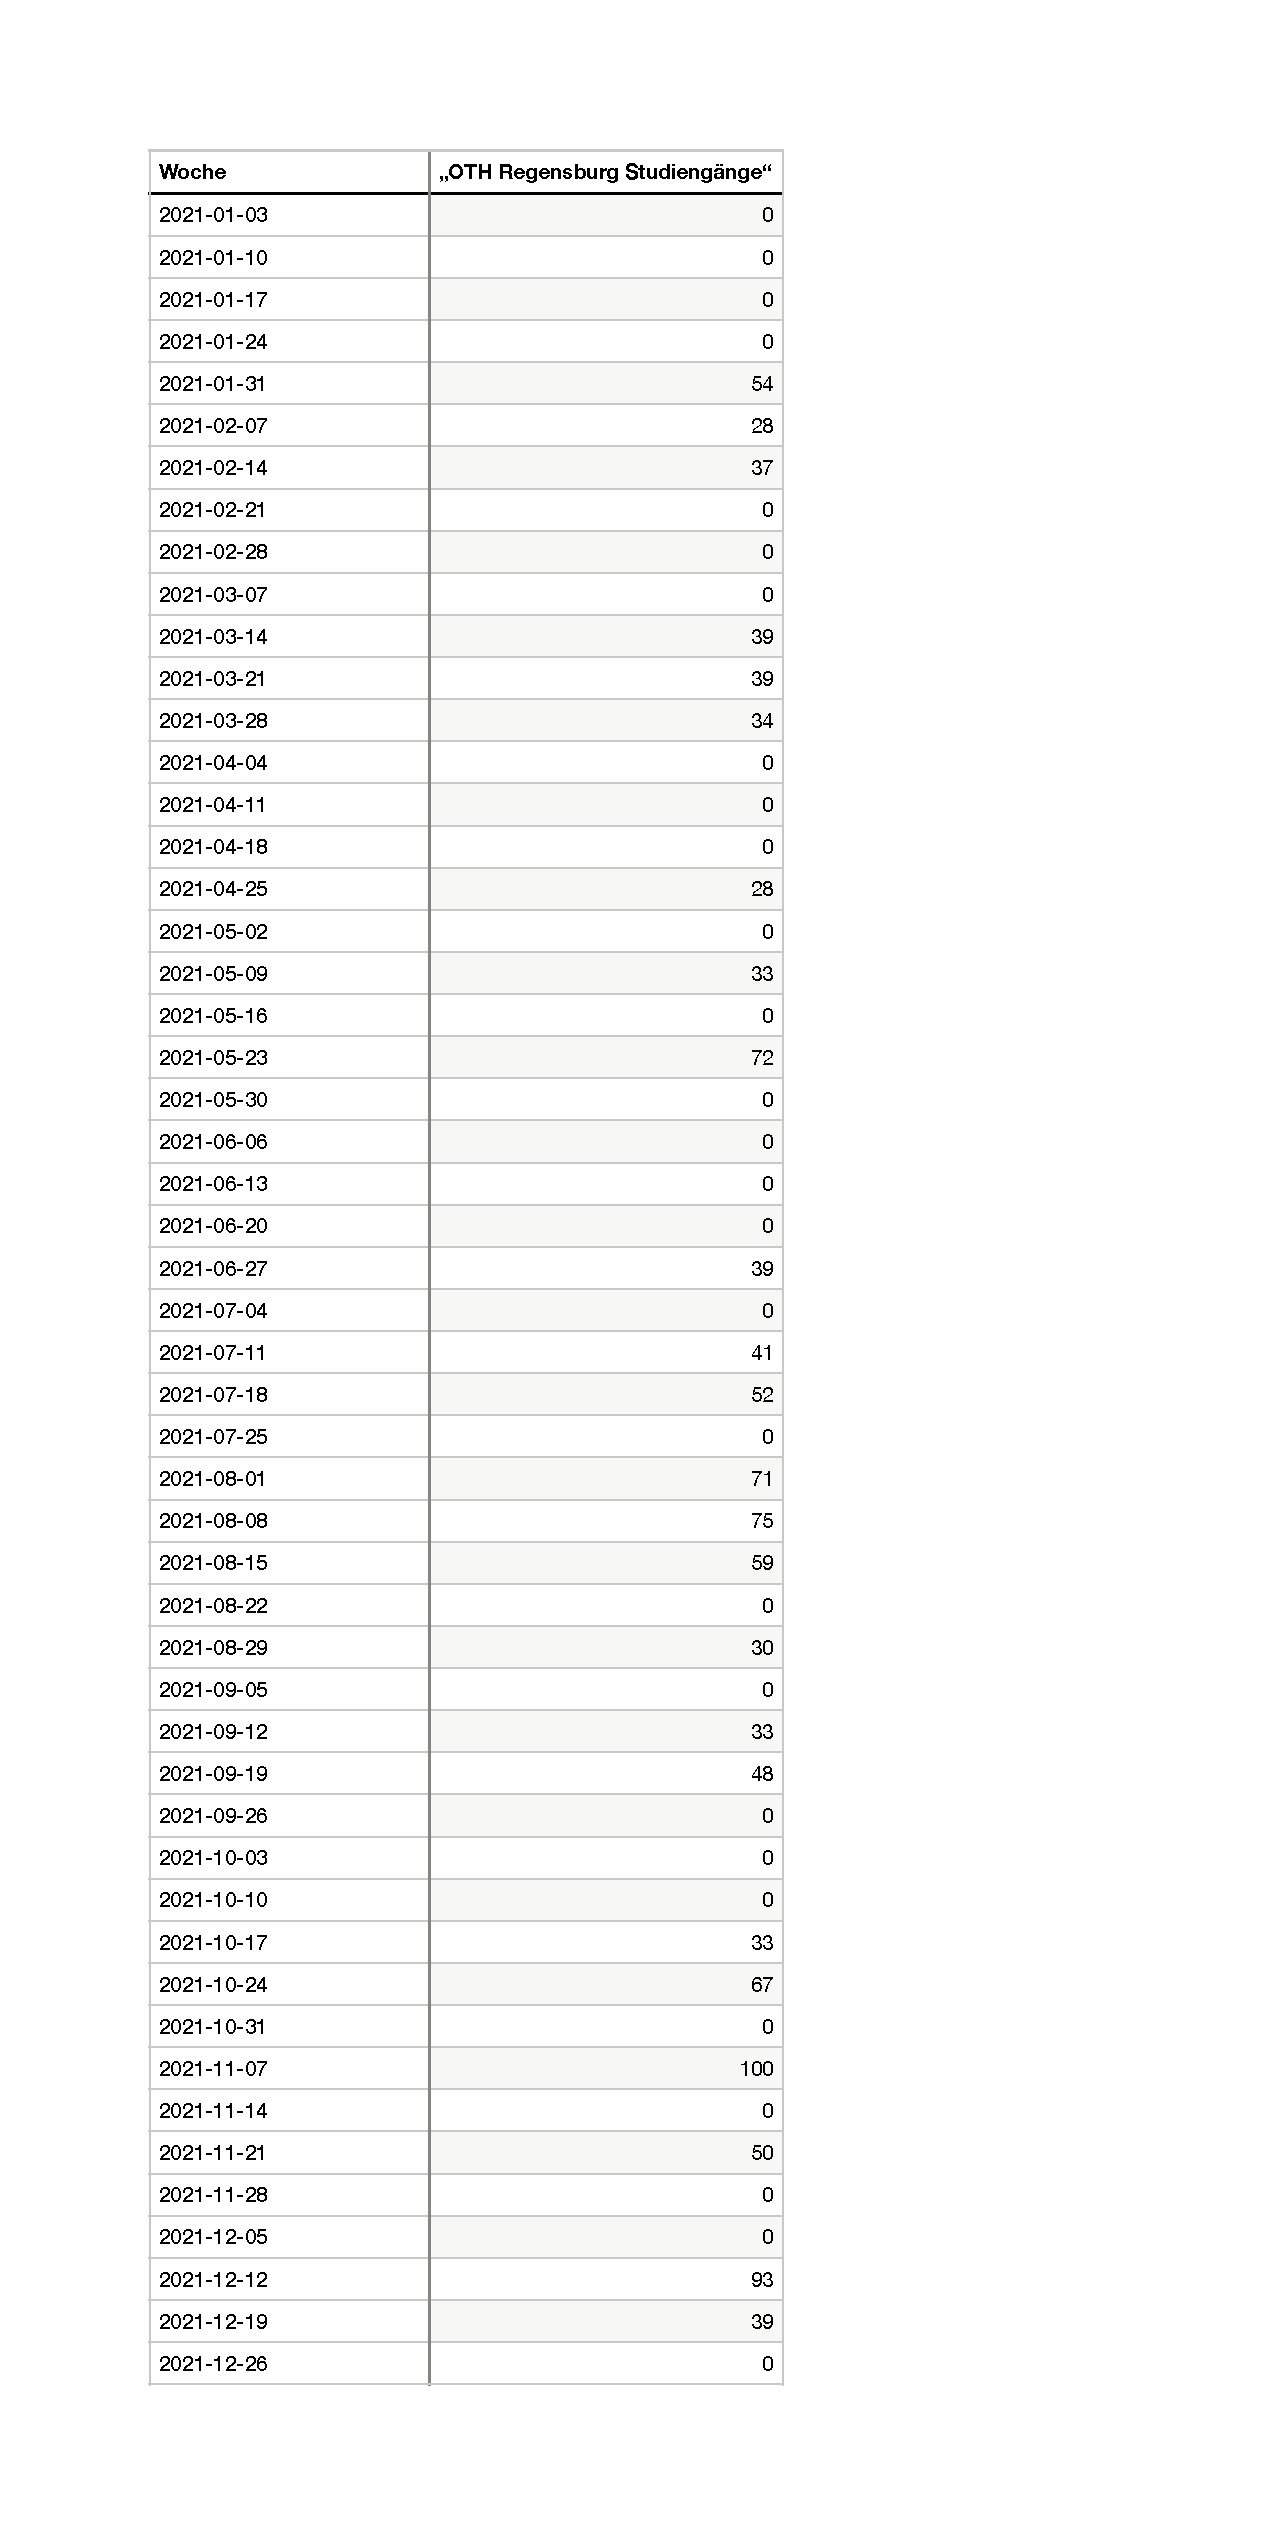
\includepdf[
    clip=0mm 0mm 0mm 0mm,
    trim=0mm 0mm 55mm 0mm,
    pages=1,
    frame,
    scale=.75,
    pagecommand=\subsection{Google Search Trends 2021: \glqq OTH Regensburg Studiengänge\grqq{}}\label{appendix:google-search-trends}
 ]{assets/pdf/google-search-trends.pdf}

\end{document}